% main.tex — Master file for University of Melbourne thesis
% University of Melbourne thesis guidelines:
% https://gradresearch.unimelb.edu.au/processes/preparation-of-graduate-research-theses
\documentclass[twoside]{uomthesis}
\usepackage[version=4]{mhchem}
\usepackage{chemformula}
\usepackage{caption}
\usepackage{float}
\usepackage[dvipsnames]{xcolor}
\usepackage{xurl}
\usepackage{amsmath} 
\usepackage{tcolorbox}
\usepackage[scaled]{FiraMono} 
\usepackage{xcolor}
\usepackage{booktabs}
\usepackage{graphicx}
\usepackage{makecell} % Required for line breaks in cells
\usepackage{textcsc}
\usepackage{nicefrac}

\PassOptionsToPackage{hyphens}{url}\usepackage{hyperref}
%--------------------------------------------%
%% Metadata %%
%--------------------------------------------%
\ThesisTitle{Gene Regulatory Network-Guided Causal Generative Modeling of Single-Cell Transcriptomics}
\ThesisAuthor{Yazdan Zinati}
%\ThesisOrcid{0000-0003-1559-6225}
\ThesisDegree{Master of Science}
\ThesisDate{February 2026}
% \ThesisResubmissionDate{Sep 2025}
\ThesisFaculty{Faculty of Engineering}
\ThesisDepartment{Department of Electrical \& Computer Engineering}
\ThesisUniversity{McGill University, Montr\'eal}
% \ThesisJointInstitution{}
\ThesisSupervisor{Amin Emad}
\usepackage{tcolorbox}
\usepackage{csquotes}
\usepackage{caption}
\DeclareCaptionLabelFormat{sflabel}{\textsf{#1~#2}}
\captionsetup[table]{labelformat=sflabel}
\captionsetup[figure]{labelformat=sflabel}

\newtcolorbox{codeblock}{
    colback=gray!10,        % light grey background
    colframe=black,         % black frame
    boxrule=0.3pt,          % thin frame
    arc=2pt,                % slightly rounded corners
    left=6pt, right=6pt,
    top=6pt, bottom=6pt,
    fontupper=\footnotesize\ttfamily  % smaller font + Fira Code
}

\let\oldtexttt\texttt
\renewcommand{\texttt}[1]{\oldtexttt{\footnotesize #1}}

\renewcommand{\UrlFont}{\ttfamily\footnotesize}


\newcommand{\figuresection}[1]{%
   \addcontentsline{lof}{chapter}{#1}%
   \addcontentsline{lot}{chapter}{#1}%
}

\usepackage{pdflscape}
\usepackage{tabularx}
\usepackage[justification=justified]{caption}
\usepackage{enumitem}

\begin{document}

  \maketitle


  %--------------------------------------------%
  %% Front matter %%
  %--------------------------------------------%
  \frontmatter
  \vspace*{\fill}
    
\includegraphics[width=0.2\linewidth]{figures/by-nc.eps}\\
    Gene Regulatory Network-Guided Causal Generative Modeling of Single-Cell Transcriptomics © 2026 by Yazdan Zinati is licensed under \textsc{cc by-nc} 4.0. To view a copy of this license, visit \href{https://creativecommons.org/licenses/by-nc/4.0/}{https://creativecommons.org/licenses/by-nc/4.0/} \\\\
    \newpage
  \chapter*{Abstract}
\addcontentsline{toc}{chapter}{Abstract} % add it to table of contents
%\vspace{-1.5em}  % adjust this value as needed
Precisely controlled programs of gene expression are essential for cellular function and organismal viability across all forms of life. Gene regulatory networks (\textsc{GRN}s) provide a high-level mathematical representation of transcriptional regulation by describing the interactions between genes and their regulatory elements, such as transcription factors, across diverse cellular states and contexts. Through this lens, \textsc{GRN}s offer biological insights into processes such as morphogenesis, disease progression, stress adaptation, and response to environmental stimuli. High-throughput profiling of gene expression, particularly single-cell RNA sequencing, has fueled the development of data-driven methods for reconstructing \textsc{GRN}s, sometimes in combination with other data modalities or omics layers. However, in the absence of comprehensive experimentally validated networks corresponding to the exact biological system and experimental conditions under study, evaluating these methods remains a major challenge. %Current \textsc{GRN}-guided simulators adopt coarse assumptions regarding TF coregulation, do not readily preserve gene identities, demand substantial user intervention, and yield benchmarks that deviate from those derived from experimental data, limiting their suitability for this task. 

In this thesis, we address key challenges in benchmarking \textsc{GRN} inference methods through two interconnected studies. \textit{Chapter 3} introduces GRouNdGAN, a \textsc{GRN}-guided simulator that achieves state-of-the-art realism in both steady-state and transient-state scRNA-seq simulations, capturing regulatory properties while preserving gene identities without requiring user intervention.  As a causal generative model, GRouNdGAN expresses genes under the control of their regulators and can sample from both observational and interventional distributions, allowing matched case/control in-silico perturbation experiments. \textit{Chapter 4} formalizes the GRouNdGAN framework as a reproducible protocol, providing in-depth procedural guidance, and introduces GRouNdGAN-toolkit, an extension of the model that includes additional features and customizable modules aimed at facilitating its adaptation to various experimental setups, which are explored through a series of new empirical studies. 

Together, these studies advance the development of \textsc{GRN} inference methods by providing synthetic gold-standard ground truths for any biological system of interest, along with procedures and tools for systematic evaluation, thereby closing the gap between in-silico and experimental data benchmarks of \textsc{GRN} inference methods. 

\newpage

\chapter*{Résumé}
\addcontentsline{toc}{chapter}{Résumé} % add it to table of contents

Des programmes d'expression génique précisément contrôlés sont essentiels à la fonction cellulaire et à la viabilité des organismes dans toutes les formes de vie. Les réseaux de régulation génique (RRG) fournissent une représentation mathématique de haut niveau de la régulation transcriptionnelle en décrivant les interactions entre les gènes et leurs éléments régulateurs, tels que les facteurs de transcription, dans divers états et contextes cellulaires. À travers ce prisme, les RRGs offrent des perspectives biologiques sur des processus tels que la morphogenèse, la progression des maladies, l'adaptation au stress et la réponse aux stimuli environnementaux. Le profilage à haut débit de l'expression génique, en particulier le séquençage d'ARN unicellulaire, a stimulé le développement de méthodes basées sur les données pour la reconstruction des RRGs, parfois en combinaison avec d'autres modalités de données ou couches omiques. Cependant, en l'absence de réseaux complets et validés expérimentalement correspondant au système biologique et aux conditions expérimentales exacts étudiés, l'évaluation de ces méthodes reste un défi majeur.

Dans cette thèse, nous abordons les principaux défis liés à l'évaluation comparative des méthodes d'inférence de RRG à travers deux études interconnectées. Le \textit{Chapitre 3} présente GRouNdGAN, un simulateur guidé par RRG qui atteint un réalisme de pointe dans les simulations scRNA-seq à l'état stationnaire et transitoire, en capturant les propriétés régulatrices tout en préservant l'identité des gènes sans nécessiter d'intervention de l'utilisateur. En tant que modèle générateur causal, GRouNdGAN exprime les gènes sous le contrôle de leurs régulateurs et peut échantillonner à partir de distributions observationnelles et interventionnelles, permettant des expériences de perturbation in silico appariées cas/témoins. Le \textit{Chapitre 4} formalise le cadre GRouNdGAN en un protocole reproductible, fournissant des instructions procédurales détaillées, et présente GRouNdGAN-toolkit, une extension du modèle qui inclut des fonctionnalités supplémentaires et des modules personnalisables visant à faciliter son adaptation à diverses configurations expérimentales, explorées à travers une série de nouvelles études empiriques.

Ensemble, ces études contribuent au développement des méthodes d’inférence des RRGs en proposant des vérités de référence synthétiques applicables à tout système biologique d’intérêt, ainsi que des procédures et des outils d’évaluation systématique, permettant ainsi de réduire l’écart entre les références in silico et expérimentales.
  \hspace{0pt}

\vspace*{\fill}
\begin{center}
To my parents, this thesis is dedicated to you for being my support through it all.
\end{center}
\vspace*{\fill}
\hspace{0pt}

\chapter*{Acknowledgments}
\addcontentsline{toc}{chapter}{Acknowledgments}

My sincere thanks go to Prof. Amin Emad for welcoming me into computational biology and guiding me through every step of this research journey.

Endless conversations, thoughtful feedback, and well-timed jokes from the members of the \textsc{combine} lab  kept this thesis on course and my sanity intact; their presence is felt in each chapter. I have been fortunate to benefit from Abdulrahman Takiddeen’s mentorship and Safyan Aman Memon’s company during late lab sessions.

The work described in this thesis was made possible thanks to the support by the Natural Sciences and Engineering Research Council of Canada (NSERC), the Government of Canada’s New Frontiers in Research Fund (NFRF), the Canada Foundation for Innovation (CFI), the McGill Initiative in Computational Medicine, Fonds de recherche du Québec, the Digital Research Alliance of Canada, and Calcul Québec.


  \tableofcontents
  
  \listoffigures     
  \listoftables  
  
  % \chapter*{Third‐Party Copyright Material}
\addcontentsline{toc}{chapter}{Third‐Party Copyright Material}




  %%% Acronyms and Glossaries %%%
  % \PrintAcronym{frontmatter/acronyms}  
  % \PrintGlossary{frontmatter/glossaries} 

  %%% Print Nomenclatures %%%
  % \PrintNomenclature{frontmatter/nomenclature}

  

  %--------------------------------------------%
  %% Load chapters %%
  %--------------------------------------------%
  \mainmatter

  \chapter*{List of Abbreviations}

\begin{singlespace}

\begin{description}[font=\textsc\bfseries, leftmargin=3cm, style=nextline]
  \item[\textsc{ae}]
   Autoencoder

\end{description}
\end{singlespace}
  %\setchapterpreamble[u]{\margintoc}
\chapter{Introduction}
%\labch{intro}


\section*{Motivation}
\addcontentsline{toc}{section}{Motivation}

Of all the macromolecules one might find in the cells of living organisms, proteins are the class which are overwhelmingly responsible for the execution of the cell's functions, operating within and beyond its borders. Proteins are at the heart of vital cell functions like metabolism, \textsc{dna} repair, cell polarity, and scaffolding.

To execute these myriad functions, proteins often participate in sometimes complex chains of chemical and physicochemical reactions with other proteins more broadly referred to as ``protein-protein interactions'' or \textsc{ppi}s. Understanding which proteins interact with other proteins is vital to our knowledge of \textit{how} cells carry-out their many functions as well as the ways in which they fail in the case of disease.

In fact, cancers and other diseases which are caused by protein mutations often result in a change in protein binding affinity, altering how those proteins interact with others \cite{Jemimah_Gromiha_2020}. Infection and diseases caused by viruses like \textsc{hiv} and \textsc{sars}-\textsc{c}o\textsc{v-2} are also carried out by interactions between host and viral proteins \cite{hiv_ppi, sars_cov2_ppi}. What's more, treatments for these diseases sometimes come in the form of so-called ``biologic'' therapies like small peptides, antibiotics, or m\textsc{rna} vaccines, which in turn carry out their functions through the same fundamental processes as \textsc{ppi}s do.

While the study of \textsc{ppi}s has immeasurably shaped our understanding of biology, the methods by which we've traditionally come to characterize them require immense investments of time, labour, and capital. These methods, which include yeast two-hybrid (\textsc{y2h}), affinity chromatography, and mass spectroscopy, are primarily conducted at the bench with the aid of specialized material, equipment, and expertise \cite{vidal_fields_2014, snider_2015, low_recent_2021}.

Consuming a fraction of the labour and capital resources, computational methods for identifying putative \textsc{ppi}s are a compelling methodology for complimenting the challenges posed by traditional experimental methods. A single \textsc{y2h} experiment, for instance, is conducted over multiple days \cite{y2h_protocol, mehla_mapping_2015}. Contrastingly, the interactions between a given protein and the entire human proteome can be conducted in approximately three minutes using the \textsc{intrepppid} method through the online \textsc{ppi}.bio portal \cite{intrepppid}. This is to make no mention of the discrepancies in capital investment between these two examples, with \textsc{y2h} requiring expensive specialist equipment and materials, while the \textsc{rapppid} \& \textsc{intrepppid} models runs on commodity computer hardware \cite{rapppid, intrepppid}.

Building upon decades of painstaking research, sizable databases of \textsc{ppi}s have been compiled across a growing number of organisms \cite{string_v12, intact}. These databases, in turn, have greatly enabled methods for identifying putative \textsc{ppi}s using data analysis and mining. Combined with the explosion of advances in the field of deep learning in recent years, it is increasingly viable for designers of \textsc{ppi} inference methods to leverage neural networks to increase benchmark accuracies.

Despite best efforts, accurate \textsc{ppi} inference that generalizes to all use-cases remains regrettably out of reach. Surprisingly prevalent and persistent challenges in the nature of training datasets and model architecture frustrate efforts to train \textsc{ppi} inference models which perform well on out-of-distribution examples \cite{park_marcotte, Hamp_Rost_2015, black_box}. While these hurdles have long been known to researchers, the challenges remain relevant and affect recent methods \cite{black_box}.

This thesis contains a collection of three studies aimed at improving \textsc{ppi} inference performance on out-of-distribution data, as well as characterizing new challenges on the horizon that threaten the generalization of tomorrow's \textsc{ppi} inference models when trained on datasets with maximum sequence identity thresholds ranging from 50\% to 90\%. 

\section*{Thesis Organization \& Contributions}
\addcontentsline{toc}{section}{Thesis Organization \& Contributions}

This thesis is organized into four additional chapters whose main technical contributions are:

\begin{itemize}
    \item \textbf{\sffamily Chapter 2} -- This thesis begins with a comprehensive review of the biological and computational literature which inform this work.
    \item \textbf{\sffamily Chapter 3} -- This chapter introduces \textsc{rapppid}, a simple model for \textsc{ppi} inference which relies on judicious applications of regularization to achieve state-of-the-art performance at the time of publication. This study also highlights that contemporaneous models fail to generalize to proteins outside the training set, and introduces tokenization typically applied to natural language to amino acids.
    \item \textbf{\sffamily Chapter 4} -- Expanding on the work done on \textsc{rapppid}, Chapter 4 reports on an investigation into leveraging orthology to further generalize \textsc{ppi} inference to unseen proteins belonging to evolutionarily-distant organisms. The resulting method, \textsc{intrepppid},  out-performs \textsc{rapppid} and other contemporaneous models when trained on human \textsc{ppi}s, and subsequently evaluated on other organisms. To do so, a novel ``orthologous locality'' loss term is defined to reshape the protein embedding latent space, ``pushing'' orthologous proteins close to one another and ``pulling'' non-orthologous proteins apart. 
    \item \textbf{\sffamily Chapter 5} -- In which we reveal a before-uncharacterized source of data leakage in \textsc{ppi} inference models which incorporate pre-trained protein large language models (p\textsc{llm}s). Furthermore, we demonstrate how careful attention to the creation of training datasets can result in p\textsc{llm}s which are both performant and do not leak data. Finally, failures to generalize across p\textsc{llm}-based and non-p\textsc{llm}-based are described.
\end{itemize}
\newpage

\section*{Publications \& Author Contributions}
\addcontentsline{toc}{section}{Publications \& Author Contributions}
\begin{itemize}
    \item \textbf{\sffamily Chapter 3}
    \begin{tcolorbox}
    Szymborski, Joseph, and Amin Emad. 2022. ``\textsc{rapppid}: Towards Generalizable Protein Interaction Prediction with \textsc{awd}-\textsc{lstm} Twin Networks.'' \textit{Bioinformatics} 38 (16): 3958–67.\\\textsc{doi}: \href{https://10.1093/bioinformatics/btac429}{10.1093/bioinformatics/btac429}.
    \end{tcolorbox}
    \textsc{a.e.} and \textsc{j.s.} conceived the study, designed the project and the algorithm, and wrote the article. \textsc{j.s.} implemented the pipeline and performed the statistical analyses of the results. All authors read and approved the final article.
    

    \item \textbf{\sffamily Chapter 4} 
    \begin{tcolorbox}
    Szymborski, Joseph, and Amin Emad. 2024. “\textsc{intrepppid}—an Orthologue-Informed Quintuplet Network for Cross-Species Prediction of Protein–Protein Interaction.” \textit{Briefings in Bioinformatics} 25 (5): bbae405. \textsc{doi}: \href{https://doi.org/10.1093/bib/bbae405}{10.1093/bib/bbae405}.
    \end{tcolorbox}

    \textsc{a.e.} and \textsc{j.s.} contributed to project conceptualization, methodology as well as writing, editing, and reviewing. \textsc{a.e.} contributed to supervision and funding acquisition. \textsc{j.s.} contributed to software, data curation, investigation and visualization. All authors read and approved the final article.
    
    \item \textbf{\sffamily Chapter 5} \\
    The manuscript in Chapter 5 is under-review and is currently available as a pre-print on the bioRxiv online pre-print repository.
    \begin{tcolorbox}
    Szymborski, Joseph, and Amin Emad. 2025. “A Flaw in Using Pre-Trained pLLMs in Protein-Protein Interaction Inference Models.” \textit{bioRxiv}. \textsc{doi}: \href{https://doi.org/10.1101/2025.04.21.649858}{10.1101/2025.04.21.649858}.
    \end{tcolorbox}

    \textsc{a.e.} and \textsc{j.s.} contributed to project conceptualization, methodology as well as writing, editing, and reviewing.
\textsc{a.e.} contributed to supervision and funding acquisition. \textsc{j.s.} contributed to software, data curation, investigation
and visualization. All authors read and approved the final article.
    

\end{itemize}

  \chapter{Background Material and Literature Review}
\label{chap:background}
\addcontentsline{lof}{chapter}{Background Material and Literature Review}

\section*{The Biological Basis of Gene Regulation}
\addcontentsline{toc}{section}{The Biological Basis of Gene Expression and Regulation}
\subsection*{Gene Expression and Transcriptional Control}
\addcontentsline{toc}{subsection}{Gene Expression and Transcriptional Control}
%Central Dogma and mRNA Abundance
%Regulation at the Transcriptional Level

\subsection*{Mechanisms of Gene Regulation and Transcription Factors}
\addcontentsline{toc}{subsection}{Mechanisms of Gene Regulation and Transcription Factors}
%TF Binding, Activation, and Repression
%Promoters, Enhancers, and Chromatin Context

\subsection*{Gene Regulatory Networks as System-Level Biological Models}
\addcontentsline{toc}{subsection}{Gene Regulatory Networks as Biological Models}
%Graph-Based Representation of Regulation (edge weights, sign, directionality,..)

\section*{Computational \& Statistical Models of Gene Regulatory Network Inference}
\addcontentsline{toc}{section}{Computational \& Statistical Models of Gene Regulatory Network Inference}

\subsection*{Problem Formulation of Gene Regulatory Network Inference}
\addcontentsline{toc}{subsection}{Problem Formulation of GRN Inference}
%Inferring Directed Networks from Expression Data
%Identifiability and Causality Challenges

% types of GRN inferene methods (, cell-specific, correlational, MI methods, Regression and Trajectory-Based (pseudotime), Structural Causal Models)

\section*{Benchmarking Gene Regulatory Network Inference Methods}
\addcontentsline{toc}{section}{Benchmarking Gene Regulatory Network Inference Methods}

\subsection*{Motivation and Challenges in Benchmarking}
\addcontentsline{toc}{subsection}{Motivation and Challenges in Benchmarking}


\subsection*{Experimental Validation-Based Benchmarks}
\addcontentsline{toc}{subsection}{Experimental Validation-Based Benchmarks}
%Perturbation-Based Experimental Benchmarks

%Binding-Based Experimental Evidence

%Curated Regulatory Databases as Benchmarks

\subsection*{Gene Regulatory-Guided Simulation}
\addcontentsline{toc}{subsection}{Gene Regulatory-Guided Simulation}


\section*{Generative Modeling and In-Silico Single-Cell Transcriptomics}
\addcontentsline{toc}{section}{Generative Modeling and In-Silico Single-Cell Transcriptomics}
\subsection*{Single-Cell Simulation}
\addcontentsline{toc}{subsection}{Single-Cell Simulation}

\subsection*{GANs, conditionalGANs and CausalGANs}
\addcontentsline{toc}{subsection}{GANs, conditi	onalGANs and CausalGANs}


% GANs
% conditional GANs
% causal GANs

% simulators for single-cell
% GRN-Guided Simulation

 
  \begin{singlespace}
\chapter*{Background and Context for ``\textit{GRouNdGAN: GRN-guided simulation of single-cell RNA-seq data using causal generative adversarial networks}''}
\markboth{Background and Context for GRouNdGAN}{Background and Context for GRouNdGAN}
\end{singlespace}

In Chapter \ref{chap:background}, I explored both the landscape of \textsc{ppi} inference methodology (Section \ref{sec:ppi_methods}), as well as their persistent and pervasive problem of these methods failing to generalize to out-of-distribution testing samples (Section \ref{sec:ppi_generalization}). It is in this context that, in 2021, my supervisor and I submitted for publication \textsc{rapppid}. Prior to \textsc{rapppid} few \textsc{ppi} inference models, and no deep learning techniques to my knowledge, were evaluated on datasets which appropriately controlled for data-leakage. Indeed, when we tested existing \textsc{ppi} inference models at the beginning of \textsc{rapppid}'s development, it became clear that models (particularly those using deep-learning methods) were still failing to generalize as Park and Marcotte observed in 2012 and Bernett \textit{et al.} would go on to observe in 2024 \cite{park_marcotte, black_box}.  

\textsc{rapppid} is a \textsc{ppi} inference model which was created to answer the question: could conventional deep \textsc{ppi} inference models be modified to overcome their failure to generalize if a focus on regularization was applied?

Inspired by then-recent studies, we began developing a \textsc{rnn}-based \textsc{ppi} inference model which incorporated \textsc{lstm}-specific regularization techniques outlined by Merity \textit{et al.} in 2017 \cite{awd_lstm}. Merity \textit{et al.}'s \textsc{awd-lstm} is a carefully tuned approach to regularizing and optimizing \textsc{rnn}s which take into consideration how traditional approaches sometimes are inappropriate for \textsc{rnn}s.

As introduced in Subsection \ref{subsec:ppi_methods_rnn}, a common problem encountered when applying \textsc{rnn} architectures is that of vanishing gradients. \textsc{rnn} variants like \textsc{lstm} and \textsc{gru}, which help to lessen the negative effects of large sequences on training stability, succumb under a number of time-steps which is even still below the average protein sequence length. While other \textsc{rnn}-based \textsc{ppi} inference methods address this limitation through the use of \textsc{cnn}s to greatly reduce the length of the sequence, we identified a few problems with this approach.

Firstly, by initially filtering sequences through the use of \textsc{cnn}s and pooling layers, the resolution of the time-steps is greatly reduced. By reducing the resolution, the \textsc{lstm}'s ability to model long-term dependencies is rendered useless, thereby squandering an opportunity to model the non-linear nature of \textsc{ppi} contact surfaces in protein sequences.  Secondly, the addition of convolutional layers added to a very constrained parameter budget. A very small number of \textsc{ppi} training pairs and a dataset which controls for data leakage makes overfitting both likely and easy to detect. For this reason, the number of parameters that make up the \textsc{rapppid} was carefully selected.

Ultimately, use of the Unigram tokenization algorithm via the Sentencepiece library allowed us to increase training stability while never bringing the resolution lower than three amino acids, grouped according to their common co-occurence  \cite{kudo_sentencepiece_2018}. Additionally, rather than contributing to overfitting, this tokenization approach had a regularization effect due to a process called ``sub-word regularization''.

The final result is a model which, achieved then-state-of-the-art accuracy on out-of-distribution evaluation datasets \cite{rapppid}. The regularization, optimization, and training modifications as applied to a fairly conventional deep \textsc{ppi} inference architecture are responsible for \textsc{rapppid}'s performance, as ablation experiments show \cite{rapppid}.

\textsc{rapppid} is proof positive that, despite a literature replete with \textsc{ppi} models that fail to generalize, it is possible to improve performance on out-of-distribution evaluation sets of simple architecture through thoughtful application of regularization and modification to the training process.

\begin{tcolorbox}
    The contents of Chapter 3 were first published on the 30\textsuperscript{th} of June, 2022 as an article of the same title in Volume 38, Issue 16 of Oxford University Press' \textit{Bioinformatics} journal and is made available under the \href{https://creativecommons.org/licenses/by/4.0/legalcode.en}{Creative Commons Attribution License}, © Joseph Szymborski and Amin Emad, 2022. \textsc{doi}: \href{https://doi.org/10.1093/bioinformatics/btac429}{10.1093/bioinformatics/btac429}
\end{tcolorbox}


\begin{singlespace}
\chapter[GRouNdGAN: GRN-guided simulation of single-cell RNA-seq data using causal generative adversarial networks]{GRouNdGAN: GRN-guided simulation of single-cell RNA-seq data using causal generative adversarial networks}
\label{chap:rapppid}
\markboth{Chapter 3: GRouNdGAN}{Chapter 3: GRouNdGAN}%
\end{singlespace}

\counterwithout{section}{chapter}
\renewcommand{\thetable}{\arabic{table}}
\renewcommand{\thefigure}{\arabic{figure}}

\figuresection{GRouNdGAN: GRN-guided simulation of single-cell RNA-seq data using causal generative adversarial networks}

\section*{Abstract}
\addcontentsline{toc}{section}{Abstract}

\textbf{Motivation:} Computational methods for the prediction of protein–protein interactions (\textsc{ppi}s), while important tools for researchers, are plagued by challenges in generalizing to unseen proteins. Datasets used for modelling protein-protein predictions are particularly predisposed to information leakage and sampling biases. \\
\textbf{Results:} In this study, we introduce \textsc{rapppid}, a method for the Regularized Automatic Prediction of Protein–Protein Interactions using Deep Learning. \textsc{rapppid} is a twin Averaged Weight-Dropped Long Short-Term memory network which employs multiple regularization methods during training time to learn generalized weights. Testing on stringent interaction datasets composed of proteins not seen during training, \textsc{rapppid} outperforms state-of-the-art methods. Further experiments show that \textsc{rapppid}’s performance holds regardless of the particular proteins in the testing set and its performance is higher for experimentally supported edges. This study serves to demonstrate that appropriate regularization is an important component of overcoming the challenges of creating models for \textsc{ppi} prediction that generalize to unseen proteins. Additionally, as part of this study, we provide datasets corresponding to several data splits of various strictness, in order to facilitate assessment of \textsc{ppi} reconstruction methods by others in the future. \\
\textbf{Availability:} Code and datasets are freely available at \href{https://github.com/jszym/rapppid}{https://github.com/jszym/rapppid} and \href{https://zenodo.org}{Zenodo.org}.\\
\textbf{Contact:} \href{amin.emad@mcgill.ca}{amin.emad@mcgill.ca}\\
\textbf{Supplementary information:} Supplementary data are available at \textit{Bioinformatics}
online.

\section{Introduction}
Interactions of proteins with other proteins and their surroundings are fundamental to the internal machinery of a cell. These interactions are of particular interest, as it is essential for a bevy of diverse cellular functions: from organizing cell structure to generating metabolic energy (Huttlin \textit{et al.}, 2017). These interactions are typically validated with a high degree of confidence by the many biological assays commonly employed today, each with their own specific advantages and challenges (Snider \textit{et al}., 2015). Assays for validating protein interactions range from the venerable yeast two hybrid (Vidal and Fields, 2014) which researchers have relied on for the past decades, to more recent Biotin-related techniques such as Bio\textsc{id-ms} (Roux \textit{et al.}, 2012). A characteristic of all these assays, however, is that they are costly in terms of time, labour and materials. A further complication of protein–protein interaction (\textsc{ppi}) studies are the multiple sources of biases that plague small and large datasets alike. Smaller datasets are particularly susceptible to `bait bias', whereby the dataset is biased by the limited and often non-random sampling of proteins studied. The proteins chosen by researchers for interaction studies often skew towards well-studied and well-annotated proteins. Larger datasets, in contrast, are often susceptible to so-called `prey bias', whereby biases in detected interactions begin to reveal themselves; be they non-specific interactions or the inability of a methodology to detect the interaction between certain proteins (Gillis \textit{et al.}, 2014). Computational approaches to predict \textsc{ppi}s are therefore useful to help towards reducing the number of costly experiments researchers are required to perform. Researchers have deployed many diverse approaches to solve the task of protein sequence-based interaction prediction. Most sequence-based methods rely on the understanding that co-evolution and co-expression of proteins are both tied to protein interaction and sequence similarity (Cong \textit{et al.}, 2019; Jansen, 2003). Some methods rely on substitution matrices for sequence alignment such as \textsc{blosum} or \textsc{pam} in combination with machine learning methods to predict interactions (Ding \textit{et al.}, 2016; Henikoff and Henikoff, 1992). Other methods utilize support vector machines (\textsc{svm}s) with kernels specifically designed for use with protein sequences (Ben-Hur and Noble, 2005). Other statistical methods including na\"ive Bayes and $k$-nearest neighbours have been used to predict protein interactions from protein sequences (Browne \textit{et al.}, 2007). Some of the most successful \textsc{ppi} prediction methods belong to the family of methods that rely on novel substring search algorithms (Dick \textit{et al.}, 2020; Li and Ilie, 2017), operating similarly to sequence search tools like \textsc{blast} (Altschul \textit{et al.}, 1990). Deep learning models have also been designed for predicting protein interactions (Chen \textit{et al.}, 2019). These deep approaches commonly either learn wide networks or share weights in a twin design; the latter being shown to be both more efficient and effective (Richoux \textit{et al.}, 2019). Such methods, however, face many challenges due to the nature of the data on which they train. Arguably, the most pervasive of which is the ability of models to generalize and predict the interactions of proteins previously unseen by the prediction method. To ensure such generalizability, careful cross-validation techniques must be used to avoid data leakage. While the necessity of appropriate cross-validation techniques is not unique to this area of research, the application of these networks (\textit{e.g.}: \textsc{ppi}s, transcriptional regulatory networks) to obtain biological insights makes it particularly important to address this challenge in the task of biological network reconstruction (Park and Marcotte, 2012; Tabe-Bordbar \textit{et al.}, 2018). For \textsc{ppi} reconstruction, developing generalizable models prove particularly difficult. The nature of \textsc{ppi} networks makes it easy to create datasets with testing/training splits which leak information, resulting in inflated performance metrics that cannot properly assess the generalizability of these methods. In particular, simply splitting interaction datasets into training and testing sets using random selection of edges results in the construction of testing datasets that are almost entirely comprised of interactions between proteins found in the training set. Indeed, Park and Marcotte (2012) found that all the \textsc{ppi} prediction models they surveyed were tested on such na\"ively constructed datasets. The surveyed models, which had optimized their performance on these na\"ive datasets that suffered from a large degree of information leakage, were also found to incur precipitous falls in their prediction metrics when tested on datasets where no proteins in the testing set occurred in the training dataset. When faced with obstacles in the construction of generalizable models, strategic and targeted applications of regularization at training time can significantly improve results. This is particularly relevant in the context of deep learning methods which pay for their expressiveness by learning an outsized number of parameters. Among the most common regularization techniques used in the deep learning context is `dropout' (Srivastava \textit{et al.}, 2014). Applying dropout to a layer consists of randomly zeroing the activations of the previous network with some probability $P$. However, choice of regularization techniques must be selected with care and in accordance with the architecture. For example, applying dropout directly to the hidden state of recurrent neural networks (\textsc{rnn}s) (Lipton \textit{et al.}, 2015), an architecture which lends itself naturally to sequential inputs such as amino acid chains, impairs its ability to retain its memory of previous inputs (Zaremba \textit{et al.}, 2015). Applying regularization to \textsc{rnn}s requires additional considerations. Recent work by Merity \textit{et al.} (2017) has demonstrated that randomly zeroing the weights of \textsc{rnn}s (`dropconnect') (Wan \textit{et al.}, 2013) rather than their hidden state activation (`dropout') effectively reduces testing error. Merity \textit{et al.} describe applying dropout to the embedding layer as well as using an averaged optimizer (non-monotonically triggered averaged stochastic gradient descent [\textsc{nt-asgd}]) as part of a series of regularization techniques dubbed Averaged Weight-Dropped Long Short-Term memory (\textsc{awd-lstm}). The regularization techniques used by \textsc{awd-lstm} models are specifically selected for their suitability in the context of training \textsc{rnn}s. To meet the generalization challenges posed by \textsc{ppi} prediction tasks, we developed a method for the Regularized Automatic Prediction of Protein–Protein Interactions using Deep Learning, or \textsc{rapppid}. \textsc{rapppid} addresses the challenges in creating generalized models for \textsc{ppi} prediction by adopting (with modification) the \textsc{awd-lstm}, a regularized \textsc{rnn} training routine (Merity \textit{et al.}, 2017). In this study, we showed that \textsc{rapppid} outperforms state-of-the-art \textsc{ppi} prediction methods on strict validation datasets constructed in accordance with guidelines set out by Park and Marcotte (2012). Additionally, we performed various analyses and applied \textsc{rapppid} to different use-cases to show case the effect of different components of its architecture and training on its performance and its applicability to different real-world scenarios. It is worth mentioning that in addition to \textsc{rapppid}'s code, we have made various pre-processed datasets freely available in the hope that they facilitate the evaluation of protein interaction prediction methods on datasets that both mitigate information leakage and are appropriately large for deep learning applications.

\section{Materials and methods}
\label{sec:rapppid:methods}

\subsection[\textsc{ppi} prediction using \textsc{awd-lstm} twin networks]{PPI prediction using AWD-LSTM twin networks}

\textsc{rapppid} is first trained by considering pairs of amino acid sequences of proteins along with a label indicating whether they do or do not interact. The amino acid sequences are first tokenized using the Sentencepiece algorithm (Kudo and Richardson, 2018), which allows for better recognition of common groupings of amino acid residues that make up the secondary structure and motifs of proteins. Fixed-length latent vector representations of the token sequences of both proteins are then computed by twin neural networks (Bromley \textit{et al.}, 1993), forming the encoder of \textsc{rapppid}’s pipeline. These twin networks have shared architectures and weights and are trained jointly. An overview of the pipeline is provided in Figure \ref{fig:rapppid:pipeline}. Each twin network consists of a two-layer bidirectional \textsc{awd-lstm} network (Merity \textit{et al.}, 2017), which takes a tokenized amino acid sequence as its input and generates a fixed-length latent vector representation as its output. \textsc{awd-lstm}s are architecturally identical to the \textsc{lstm}s (Hochreiter and Schmidhuber, 1997); however at inference time, several regularization techniques are employed while training to promote learning generalized weights. Among these regularization techniques are an averaged optimizer and dropout applied to embeddings and \textsc{lstm} weights (Athiwaratkun \textit{et al.}, 2019; Wan \textit{et al.}, 2013). Using an \textsc{awd-lstm} encoder enables \textsc{rapppid} to leverage the strong inductive biases of \textsc{lstm}s, while ensuring that the learned weights are generalized. The final hidden state of the \textsc{awd-lstm} is passed to a single fully connected layer whose output, once activated by the Mish function (Misra, 2020), is the latent representation of the amino acid sequences. The latent representations of both proteins are then concatenated and provided as inputs to the classifier network which generates an interaction probability for each protein pair. The classifier network is a two-layer fully connected network that outputs a single logit whose sigmoid activation serves as the probability of the two proteins interacting. The activated logit is then used to calculate the mean binary cross-entropy loss. Relegating the pairwise comparison of proteins to the shallower classifier network allows \textsc{rapppid} to infer protein interactions in an efficient manner. Figure \ref{fig:rapppid:pipeline} provides an overview of \textsc{rapppid}'s pipeline.

\begin{figure}%figure1
	\centerline{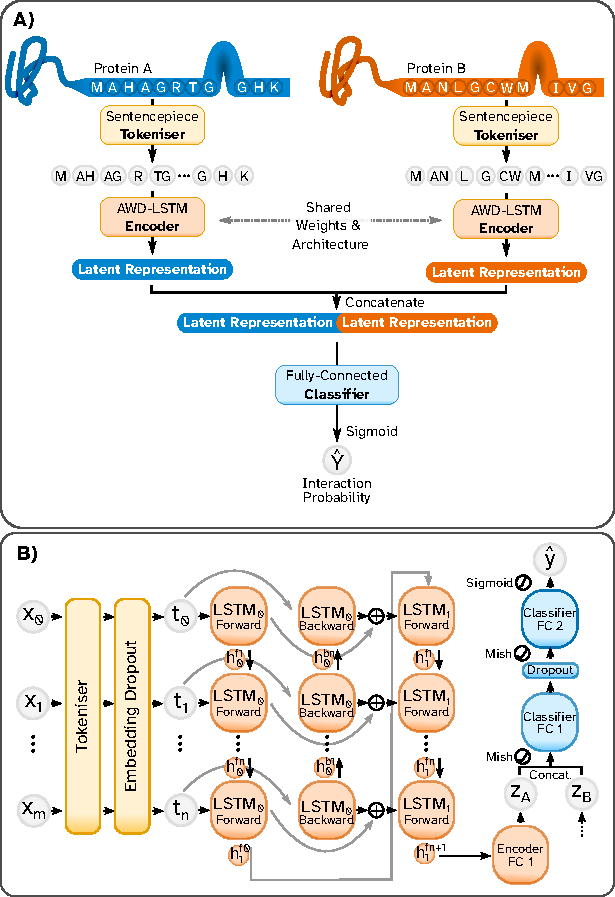
\includegraphics[scale=1]{figures/rapppid/overview_panel.pdf}}
	\caption[Overview of the \textsc{rapppid} pipeline and architecture.]{\textsf{\textbf{Overview of the RAPPPID pipeline and architecture.}} \textbf{(A)} The pipeline of the \textsc{rapppid} begins with two protein sequences. Each sequence is first tokenised by the Sentencepiece tokeniser (yellow). Each sequence of tokens is then inputted separately into an \textsc{awd-lstm} encoder layer which results in a latent representation for each protein. The latent representations of each protein are inputted into a fully-connected classifier layer. The classifier layer outputs the predicted probability of the two proteins interacting. \textbf{(B)} Taking a closer look at the architecture of the \textsc{rapppid}, individual residues $x_0$ to $x_m$ for a protein comprised of $m$ residues are tokenized into $n$ tokens $t_0,t_1,\dots,t_n$. The embedding dropout layer randomly assigns random tokens from the total vocabulary to zero. The encoder layer is comprised of a multi-layer bidirectional \textsc{lstm} whose last hidden state is fed to a fully connected layer before outputting a latent representation $z_A$. $z_A$ is then concatenated with the latent representation of a second protein ($z_b$) before being inputted into the two-layer fully-connected classifier. The output of the classifier is activated by the sigmoid function to produce a probability of interaction.}\label{fig:rapppid:pipeline}
\end{figure}

\subsection{Sequence segmentation and tokenization}

As mentioned earlier, \textsc{rapppid} utilizes the Sentencepiece algorithm (Kudo and Richardson, 2018) to tokenize amino acid sequences. While words form the basis of many natural languages and may break up sentences and phrases into discrete units, no such higher-order segmentation is as immediately apparent in amino acids. Motifs and protein domains possess many analogous qualities to words in natural languages; they appear repeatedly in amino acid sequences and their combination and relative position in these sequences play important roles in the protein structure and function (Anfinsen, 1973). Much like words, however, motifs and protein domains present an `out-of-vocabulary' problem, where unseen examples are difficult to handle. Attempts to solve this problem in natural language processing tasks have resulted in `subword' segmentation algorithms, particularly in difficult-to-segment languages such as Japanese which do not separate words by spaces (Schuster and Nakajima, 2012). Here, we employ the Sentencepiece algorithm (Kudo and Richardson, 2018) to sample tokens from `subword' vocabularies generated by the Unigram algorithm (Kudo, 2018). The Unigram and Sentencepiece algorithms construct vocabularies of arbitrary size by modelling the probabilities of subwords and provides a principled manner for sampling from this distribution to reconstruct sequences. The multi-residue tokens that comprise the vocabulary subdivide low-entropy areas and reduce the overall length of the sequences encoded.

\subsection[Generalizing protein sequence encoding with \textsc{awd-lstm}]{Generalizing protein sequence encoding with AWD-LSTM}

The task of \textsc{ppi} prediction on unseen proteins is a difficult problem prone to overfitting, as demonstrated by the poor testing performance of various methods on unseen proteins (Park and Marcotte, 2012). For this reason, a training and optimization methodology that allows efficient regularization is desirable. \textsc{awd-lstm} was recently devised to enable efficient training of generalizable \textsc{rnn}s (Merity \textit{et al.}, 2017). This approach deploys several regularization techniques during training to achieve this goal. \textsc{rapppid} adopts, with modification, the training methodology of \textsc{awd-lstm}. \textsc{rapppid} utilizes Embedding Dropout, DropConnect (Wan \textit{et al.}, 2013) and Weight Decay (Loshchilov and Hutter, 2019) on the \textsc{lstm} weights, as described by \textsc{awd-lstm}, in the encoder during training. Both \textsc{awd-lstm} and \textsc{rapppid} optimize over average weights; however, the optimizers are quite different. \textsc{awd-lstm} makes use of the \textsc{nt-asgd} optimizer which switches between \textsc{sgd} and the \textsc{asgd} variant. \textsc{rapppid} uses the recent stochastic weight averaging (\textsc{swa}) strategy in combination with the Ranger21 optimizer (Athiwaratkun \textit{et al.}, 2019; Wright and Demeure, 2021). \textsc{swa} has been shown to promote generalizable models in part by overcoming the challenges of finding best solutions within flat loss basins (Izmailov \textit{et al.}, 2019). Ranger21 is an optimizer that applies the `Lookahead mechanism' (Zhang \textit{et al.}, 2019) to the AdamW optimizer (Loshchilov and Hutter, 2019) and includes several optimization techniques (Wright and Demeure, 2021). These techniques, which include gradient centralization and adaptive gradient clipping, enable us to further improve our ability to learn generalized weights and smooth training trajectories (Brock \textit{et al.}, 2021; Yong \textit{et al.}, 2020). Finally, since \textsc{rapppid} does not rely on the timestep outputs of the \textsc{lstm} network, the temporal regularization described by \textsc{awd-lstm} is not applied.

\subsection[Details of \textsc{rapppid}’s architecture and hyper-parameter tuning]{Details of RAPPPID’s architecture and hyper-parameter tuning}

The dimensionality of the \textsc{awd-lstm} hidden state is made equal to the dimensionality of the embeddings (\textit{i.e.}: 64). The output of the fully connected layer is of equal dimensionality to that of the \textsc{awd-lstm} hidden state and is activated by the Mish activation function (Misra, 2020). The output of the first fully connected layer is half the size of the embedding dimension, activated by the Mish function and regularized by a dropout layer (Srivastava \textit{et al.}, 2014). \textsc{rapppid} trains on a vocabulary of 250 tokens that is generated by the Sentencepiece algorithm. New vocabularies are generated for each dataset before training. The number of \textsc{lstm} layers, \textsc{l2} coefficient and various dropout rates are defined as hyper-parameters that require tuning between different datasets. Hyper-parameters were selected by cross-validation. The range of considered hyper-parameters and their selected values are provided in Supplementary Tables \ref{tab:rapppid_hyperparam_range} and \ref{tab:rapppid_hyperparams}. The chosen hyper-parameter ranges are a compromise between common, reasonable values and maintaining a manageable hyper-parameter space which can be explored practically.

\subsection{Protein interaction datasets}

We obtained \textsc{ppi}s and protein sequences from version 11 of the Search Tool for the Retrieval of Interacting Genes/Proteins (\textsc{string}) database (Szklarczyk \textit{et al.}, 2019), from the official \textsc{string} website. Edges were downloaded from \href{https://stringdbstatic.org/download/protein.links.detailed.v11.0.txt.gz}{https://stringdbstatic.org/download/\\protein.links.detailed.v11.0.txt.gz} and sequences were downloaded from \\\href{https://stringdb-static.org/download/protein.sequences.v11.0.fa.gz}{https://stringdb-static.org/download/protein.sequences.v11.0.fa.gz}. In this dataset, the association between any two proteins is assigned a confidence score depending on the source of the information (called a `channel'). In our analyses, only associations with a combined \textsc{string}-score above 95\% (equivalent to a score above 950, obtained from combining different channels) were considered as positive edges. We also retained the channel specific scores for further analysis. To obtain an estimate of the false-positive rate of the confidence score-filtered \textsc{string} dataset, we leveraged the curated and experimentally validated non-interacting protein pairs from the Negatome dataset (Blohm \textit{et al.}, 2014). By comparing the set of proteins that are in both \textsc{string} and Negatome, and evaluating the number of negative edges in Negatome that were considered a positive edge in this intersection, we estimated the false-positive rate of our \textsc{string} dataset to be 4.01\%. This false-positive rate is within the expected 5\% upper-bound given by our 95\% confidence threshold. \textsc{ppi} graphs are understood to be scale-free in the general case. This property of \textsc{ppi} graphs can make them challenging datasets upon which to train a generalized model, as some proteins can be over-represented. To characterize the extent to which proteins are represented in the dataset, we calculated the distribution of the relative degree of proteins in the network (Supplementary Fig. \ref{tab:rapppid_hyperparam_range}A–C). The vast majority of proteins (upwards of 85\%) have edges with fewer than 1\% of proteins within their dataset split (\textit{i.e.}: train/validation/test). The protein with the highest degree is \textit{CDC5L} which has a relative degree of just over 10\%, while the second highest has a relative degree of 6.2\% (Supplementary Fig. \ref{tab:rapppid_hyperparam_range}D–F).

\subsection{Negative examples}

The preparation of datasets of pairs of proteins which are known not to interact with one another is a fraught process. Various methods are typically deployed to create such datasets, which are integral for machine learning methods as they typically require negative examples. Ideally, only negative examples are entirely composed of non-interacting protein pairs which are experimentally verified and manually curated, such as the Negatome database (Blohm \textit{et al.}, 2014).

Unfortunately, non-interacting pairs are difficult to experimentally validate. As a result, there are far fewer \textit{Homo~sapiens} negative protein pairs in such datasets as Negatome than positive protein pairs in databases such as \textsc{string}. Precisely, there are 1~191 negative \textit{H.~sapiens} pairs in Negatome, and 263~130 positive pairs above a 95\% confidence threshold in \textsc{string} (only pairs comprised of proteins present in Uniprot\textsc{kb} were included in this analysis). The resulting class imbalance is detrimental to learning performant, generalizable models.

Synthetic negative pairs are often used to compensate for the small number of experimentally verified non-interacting pairs is construction of synthetic negative pairs. A common method for constructing negative pairs is to select pairs of proteins from distinct sub-cellular compartments. This method has unfortunately been shown to result in biased samples according to multiple measures (Ben-Hur and Noble, 2006). Selecting pairs at random from the space of pairs not known to interact has proven to evade such biases, but runs the risk of capturing yet unknown false negatives. Unless otherwise noted, \textsc{rapppid} utilizes synthetic random pairs of proteins which are not known to interact.

\subsection{Training, validation and testing set construction}

As identified by Park and Marcotte (2012), methods which consider the interaction of proteins in a pairwise fashion must (and have historically failed to) take additional care to avoid information leakage when constructing training and testing datasets. Following their suggestion, here we use three different classes of testing and training sets to evaluate the performance of \textsc{rapppid} and other algorithms (Fig. \ref{fig:rapppid:channels}).

\begin{enumerate}
\item{`\textsc{c1}' refers to the evaluation scheme in which edges (pairs of proteins) are randomly selected to form the training or testing sets. Since the selection criterion is based on edges, both proteins in the pair may be present in both the testing and training sets (due to the presence of other edges adjacent to each protein).}
\item{`\textsc{c2}' refers to the evaluation scheme in which proteins are randomly selected to form the training or testing sets. In this scheme, only one protein in a pair may be present in both testing and training sets (but never both). This evaluation scheme mimics the scenario in which a model trained on the interactome is used to predict the interaction of known proteins with a newly discovered protein (that was not used to train the model).}
\item{`\textsc{c3}' refers to the evaluation scheme in which proteins are randomly selected to form the training or testing sets. However, unlike \textsc{c2}, proteins which appear in the training set never appear in the testing set. This is the most strict evaluation scheme.}
\end{enumerate}

While most methods have typically reported on models validated with datasets in the \textsc{c1} class, they often perform much worse on similar datasets in the more conservative \textsc{c2} and \textsc{c3} classes. This is likely due to the information leakage between training and testing sets present in the \textsc{c1} class and, to a lesser extent, in the \textsc{c2} class. In our evaluations, we report the performance of different methods using all three evaluation schemes above, but we are most interested in the results of \textsc{c3} due to a lack of information leakage. In the C-type datasets we’ve created, there are 9~300 proteins. The number of edges in the datasets ranges from just over 263~000 edges in the \textsc{c1} dataset to just under 174~000 edges in the \textsc{c3} dataset. Full dataset statistics are presented in Supplementary Table \ref{tab:rapppid_data_stats}. These C-type datasets are made freely available to the public through the Zenodo repository at \href{https://doi.org/10.5281/zenodo.6709790}{https://doi.org/10.5281/zenodo.6709790} (Szymborski and Emad, 2022a). We’ve made these datasets available in the hope that it facilitates the evaluation of protein interaction prediction methods on datasets that both mitigate information leakage and are appropriately large for deep learning applications. The adoption of C-type datasets for training and evaluation of \textsc{ppi} prediction methods is important for accurate and representative benchmarking.

\subsection{Implementation}

\textsc{rapppid} was implemented in the Python computer language using the PyTorch and PyTorch Lightning deep learning framework (Falcon \textit{et al.}, 2020; Paszke \textit{et al.}, 2019). Embedding Dropout and DropConnect implementation were obtained from the \textsc{awd-lstm} code base (Merity \textit{et al.}, 2017). The source code for \textsc{rapppid} can be found by visiting \href{https://github.com/jszym/rapppid}{https://github.com/jszym/rapppid} or through the Zenodo repository at \href{https://doi.org/10.5281/zenodo.6709213}{https://doi.org/10.5281/zenodo.6709213} (Szymborski and Emad, 2022b). \textsc{rapppid} was trained at a rate of 2.7 training steps per second at a batch size of 80 protein pairs on an Nvidia \textsc{rtx} 2080 \textsc{gpu} and 32 \textsc{cpu} cores clocked at 2.2 GHz. The \textsc{c3} model takes 2.4 h to train, while \textsc{c1} and \textsc{c2} take 7.8 h.

\begin{figure}[]%figure2
	\centerline{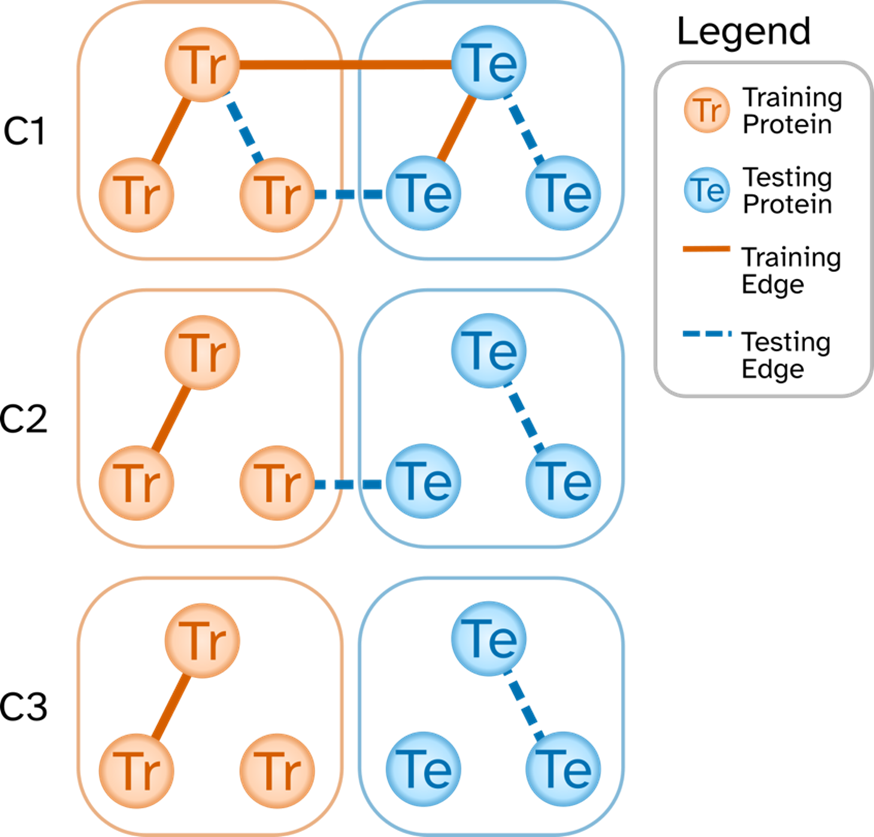
\includegraphics[scale=0.75]{figures/rapppid/c_datasets.png}}
	\caption[Illustration of differences in edges between \textsc{c1}, \textsc{c2}, and \textsc{c3} datasets.]{\textsf{\textbf{Illustration of differences in edges between C1, C2, and C3 datasets.}} Differences between \textsc{c1}, \textsc{c2}, and \textsc{c3} datasets are most visible by first dividing the population of all proteins in the dataset into training (orange, left) and testing (blue, right). In the case of the strict \textsc{c3} dataset (bottom row), edges known at training time (orange, solid) only occur between training proteins. Similarly, \textsc{c3} datasets are evaluated on testing edges (blue, dotted) that only occur between testing proteins. The \textsc{c2} dataset has all the edges present in the \textsc{c3} dataset, but also includes testing edges between testing proteins and training proteins. Finally, the pervasive \textsc{c1} datasets allows all possible training and testing edges that are not identical.}\label{fig:rapppid:c_dataset}
\end{figure}

\subsection{Protein similarity experiments}

In the analysis of the sequence similarity between testing and training proteins, ‘Percent Identity’ was measured between proteins using \textsc{ncbi}’s \textsc{psi-blast} tool running locally as part of version 2.12.0 of \textsc{ncbi}'s \textsc{blast}+ software suite (Altschul \textit{et al.}, 1997). In addition to the Percent Identity, for two proteins to be considered similar, an E-value cut-off of at most 5 and an alignment length of more than 30\% of the query sequence were considered necessary. The 64-bit Linux binaries of the \textsc{blast}+ suite were obtained from the link \\\href{ftp://ncbi.nlm.nih.gov/blast/executables/blast+/2.12.0/}{ftp://ncbi.nlm.nih.gov/blast/executables/blast+/2.12.0/}.

\section{Results}

\subsection[Performance evaluation of \textsc{rapppid} and other algorithms]{Performance evaluation of RAPPPID and other algorithms}

To establish the ability of \textsc{rapppid} to correctly predict \textsc{ppi}s within the current landscape of \textsc{ppi} prediction methods, we compared it against three recent methods (Fig. \ref{fig:rapppid:auroc}). The first of these is the Scoring Protein INTeractions (\textsc{sprint}) method, which belongs to the family of methods that predict interactions according to measures of sequence similarity (Li and Ilie, 2017). \textsc{sprint} was shown to outperform \textsc{svm}, random forest and sequence similarity-based methods across \textsc{c1}, \textsc{c2} and \textsc{c3}-like datasets.

The two other methods, \textsc{pipr} and Deep\textsc{ppi}, are deep learning methods that similar to \textsc{rapppid} utilize twin networks (Chen \textit{et al.}, 2019; Richoux \textit{et al.}, 2019). \textsc{pipr} uses a residual recurrent convolutional neural network for its encoder with the goal of more effectively summarizing both local and global features. We compared \textsc{rapppid} against the best performing iteration of Deep\textsc{ppi}, whose encoder comprises of a convolutional neural network feature extractor followed by an \textsc{lstm} network. All three methods required retraining, as the available weights of these models belong to diverse datasets, all of which are either not \textsc{c2} or \textsc{c3} type, or (in the case of \textsc{sprint}) are insufficiently large for training a generalized deep learning model. Across \textsc{c1}, \textsc{c2} and \textsc{c3} testing datasets, \textsc{rapppid} achieved higher area under the receiver-operator curve (\textsc{auroc}) than all other methods tested (Table~\ref{Tab:auroc}). The margin between \textsc{rapppid} and the second highest performing method (\textsc{sprint} in all cases) was highest when performed on the stricter \textsc{c3} dataset, resulting in 24.3\% improvement. The improvement obtained by \textsc{rapppid} compared to \textsc{sprint} was lower on the \textsc{c2} dataset (3.4\%), and finally nearly equivalent on the least strict \textsc{c1} dataset. With regards to the area under the precision-recall curve (\textsc{aupr}), this trend across dataset types persisted. \textsc{rapppid}’s \textsc{aupr} was higher than all other methods for the \textsc{c3} dataset, with a margin to the second highest method of 0.094 (equivalent to a 14.6\% improvement). \textsc{rapppid}’s \textsc{aupr} score was matched by \textsc{sprint} in experiments conducted on the \textsc{c2} dataset, but outperformed Deep\textsc{ppi} and \textsc{pipr}. \textsc{sprint} achieved the highest \textsc{aupr} of all the methods in the \textsc{c1} dataset, outperforming \textsc{rapppid} with a margin of 0.009 (equivalent to a 0.9\% improvement). 

\begin{table}[!t]
	\caption[Comparison of \textsc{ppi} prediction performance on \textsc{c1}, \textsc{c2}, and \textsc{c3} datasets.]{\textbf{\textsf{Comparison of PPI prediction performance on C1, C2, and C3 datasets.}}
    \label{tab:rapppid:auroc}} {
    \begin{center}
    \begin{tabular}{@{}llll@{}}\toprule 
			Dataset & Method & Testing \textsc{auroc} & Testing \textsc{aupr}\\\midrule
			\textsc{c1} & \textsc{rapppid} & \textbf{0.978} & 0.974\\
			    & \textsc{sprint} & 0.977 & \textbf{0.983}\\
			    & Deep\textsc{ppi} & 0.874 & 0.881\\
			    & \textsc{pipr} & 0.501 & 0.405\\\midrule
			\textsc{c2} & \textsc{rapppid} & \textbf{0.859} & \textbf{0.868}\\
			   & \textsc{sprint}  & 0.830 & \textbf{0.868}\\
			   & Deep\textsc{ppi} & 0.760 & 0.787\\
			   & \textsc{pipr} & 0.507 & 0.508\\\midrule
			\textsc{c3} & \textsc{rapppid} & \textbf{0.803} & \textbf{0.810}\\
			   & \textsc{sprint}  & 0.646 & 0.716\\
			   & Deep\textsc{ppi} & 0.574 & 0.590\\
			   & \textsc{pipr} & 0.505 & 0.509\\
			\midrule
	\end{tabular}
    \\\\
    {\footnotesize Note: The testing AUROC and AUPR of four different PPI prediction methods is reported across the three different dataset types described by Park and Marcotte (Park and Marcotte, 2012). The highest value for each dataset are reported in boldface.}
    \end{center}
    }{}
\end{table}

While we were able to replicate results of the \textsc{pipr} model on the \textit{Saccharomyces cerevisiae} dataset published as part of the original \textsc{pipr} publication (Chen \textit{et al.}, 2019), \textsc{pipr} suffered from convergence issues during training on our \textit{H.~sapiens} \textsc{string} datasets. We suspect this is due to a variety of factors, with the large differences in dataset characteristics being the most likely cause. The number of proteins and interactions in the \textit{S. cerevisiae} dataset is far smaller than our \textsc{string} datasets. Furthermore, the \textit{S. cerevisiae} dataset selected pairs of proteins which occupy different sub-cellular compartments in order to construct negative samples; an approach found to lead to biased estimations of prediction accuracy (Ben-Hur and Noble, 2006). Taken together, these results suggest that \textsc{rapppid} outperforms alternative methods in the majority of evaluations on \textsc{c1}, \textsc{c2} and \textsc{c3} schemes and is particularly effective in the stricter and more difficult \textsc{c3} evaluation.

\begin{figure*}[b!]%figure3
	\centerline{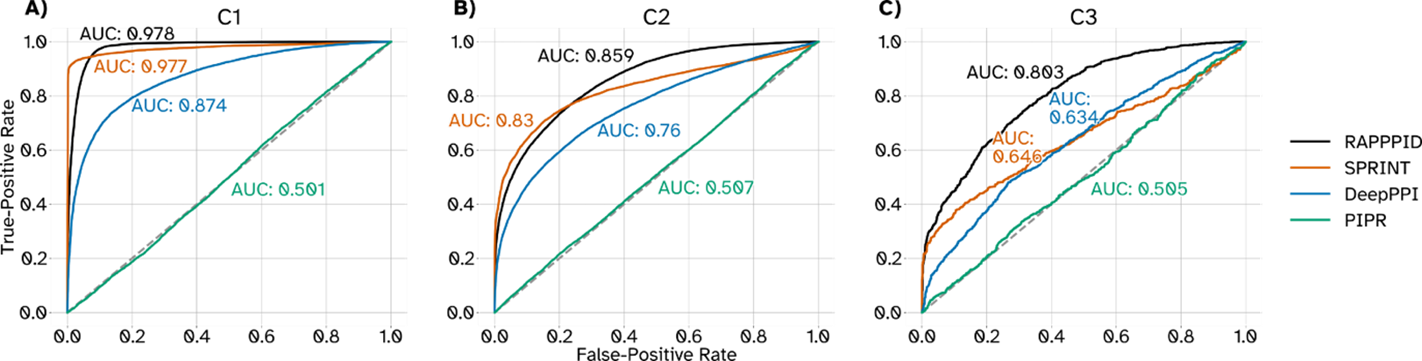
\includegraphics[scale=0.9]{figures/rapppid/auroc.png}}
	\caption[Receiver-Operator curves across methods and datasets.]{\textsf{\textbf{Receiver-Operator curves across methods and datasets.}} The receiver-operator curves (\textsc{roc}s) for all four methods tested across \textsc{c1} \textbf{(A)}, \textsc{c2} \textbf{(B)}, and \textsc{c3} \textbf{(C)} datasets.}\label{fig:rapppid:auroc}
\end{figure*}

\subsection[Channel-specific performance of \textsc{rapppid}]{Channel-specific performance of RAPPPID}

The \textsc{string} database, integrates and annotates protein association data from a wide range of sources. The `database', `text-mining', `experiments' and `co-expression' channels make up the majority of the edges in our datasets (\textit{e.g.}: 98.4\% of all the edges in the \textsc{c3} dataset). The `database' channel is comprised of several curated databases of interactions such as \textsc{kegg} and Reactome (Jassal \textit{et al.}, 2019; Kanehisa and Goto, 2000). Edges in the `text-mining' channel are the result of a statistical analysis of proteins whose names and/or identifiers co-occur in publications. The `experiments' channel is populated by interactions evidenced by high-throughput experiments curated by members of the International Molecular Exchange (\textsc{ime}x) consortium (Orchard \textit{et al.}, 2012). This includes datasets such as IntAct, \textsc{dip}, the Bio\textsc{grid} and many others (Orchard \textit{et al.}, 2014; Oughtred \textit{et al.}, 2021; Salwinski \textit{et al.}, 2004). Finally, the `coexpression' channel arises from proteomic and transcriptomic assays which quantify gene-by-gene correlations. \textsc{string} additionally assigns calibrated confidence scores to each of the edges which summarize the evidence supporting an edge. Scores are assigned to each edge by channel, and finally harmonized into a final ‘combined confidence score’ which represents the evidence across all channels present in ‘\textsc{string}’. To better characterize the results of our protein-protein prediction tests, we sought to identify the source of the testing edges \textsc{rapppid} correctly and incorrectly identified. Figure \ref{fig:rapppid:channels}A and Supplementary Figure \ref{fig:rapppid:channels_supp} show that \textsc{rapppid} can accurately predict the testing set edges that have a high confidence score in biologically supported channels of co-expression, experiments, and database. However, the accuracy for the edges that have a high confidence score in the text-mining channel is inferior to the other channels. Since edges that are only supported by text-mining (but not by the other channels) are arguably the ones most prone to error, we expected \textsc{rapppid} to have an inferior performance on such edges (since the edges themselves may not be reliable). To test whether the inferior performance of \textsc{rapppid} in the text-mining channel in Figure \ref{fig:rapppid:channels}A is indeed due to such edges, for a fixed threshold $k$ ($50\leq k \leq 95$), we divided the testing edges with a text-mining confidence score at least equal to $k$ into two groups: a group with `experiments' confidence score at least equal to 80\% and a group with `experiments' confidence score smaller than 80\% (Fig. \ref{fig:rapppid:channels}B). Evaluating the testing edges in \textsc{c1}, \textsc{c2} and \textsc{c3} showed that for this channel, the accuracy on the former group is higher than the latter group (sometimes as large as 22\% higher, Supplementary Fig. \ref{fig:rapppid:channels_supp2}). Repeating the analysis for co-expression and database channels also confirmed this trend (Fig. \ref{fig:rapppid:channels}B and Supplementary Fig. \ref{fig:rapppid:channels_supp2}). Taken together, these results suggest that the inferior performance of \textsc{rapppid} on the text-mining channel in Figure \ref{fig:rapppid:channels}A is indeed due to the edges that are supported only by text-mining and not by other biologically identified channels.

\begin{figure}[h!]%figure4
	\centerline{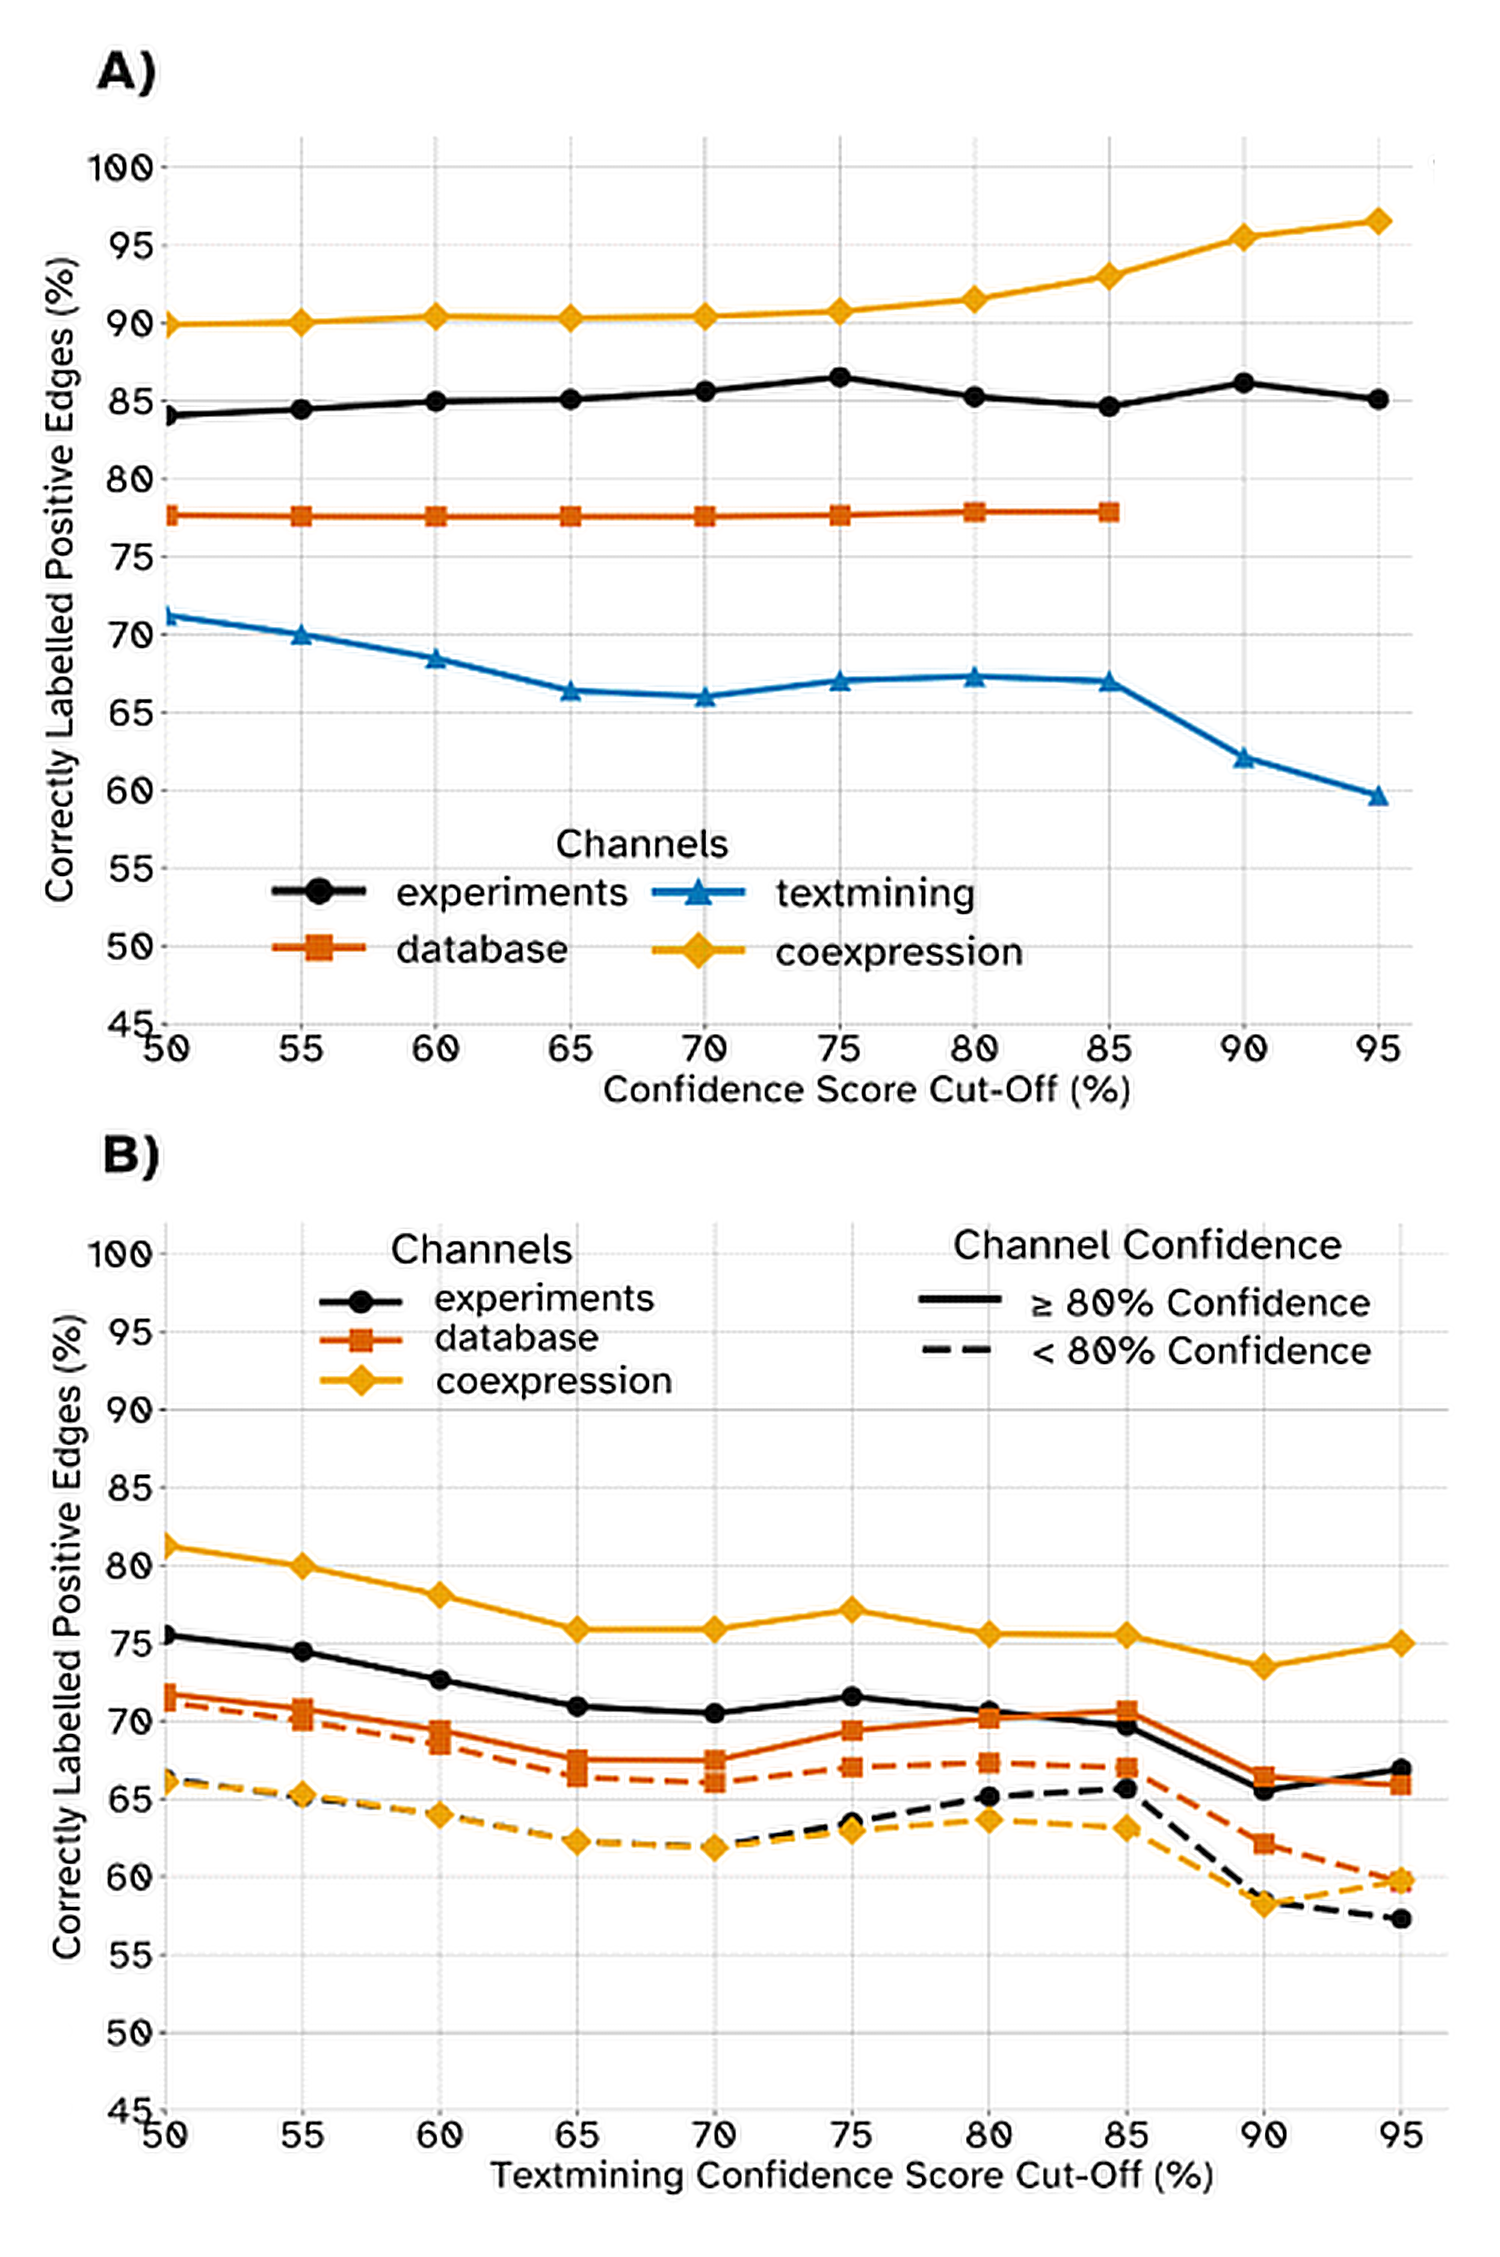
\includegraphics[scale=0.5]{figures/rapppid/channels.png}}
	\caption[Accuracy of positive edges across edge confidence stratified by \textsc{string} channels.]{\textsf{\textbf{Accuracy of positive edges across edge confidence stratified by \textsc{string} channels.}} \textbf{(A)} The percentage of correctly labelled positive edges are plotted for each major \textsc{string} channel. The x-axis denotes the channel edge confidence cut-off score for each curve’s respective channel. \textbf{(B)} Here, we see a similar chart but rather than using each channel’s respective score as a confidence cut-off, edges are excluded according to their text-mining confidence (x-axis). The solid curves include edges which have a channel confidence \hbox{$\geq$80\%}  for the channel indicated by the curve’s colour. Dashed curves conversely include edges whose channel confidence is 80\% for the channel indicated by the curve’s colour.  In both \textbf{(A)} and \textbf{(B)} data shown reflects the \textsc{c2} model/dataset.}\label{fig:rapppid:channels}
\end{figure}

\subsection[Role of protein similarity on \textsc{rapppid}’s performance]{Role of protein similarity on RAPPPID’s performance}

The procedures for \textsc{c2} and \textsc{c3} datasets were devised to reduce the information leakage by avoiding testing on edges which contain proteins which are known to an algorithm during its training. This safeguard against information leakage, however, does not account for proteins which are known by different identifiers but share near identical protein sequences. Further complicating the matter, sequence similarity is a valid \textsc{ppi} prediction feature and is often used by methods as a proxy measure of co-evolution and conserved functional domains (Cong \textit{et al.}, 2019; Jansen, 2003). Indeed, this strategy is leveraged by the \textsc{sprint} algorithm against which \textsc{rapppid} was compared.

In spite of the challenges above, we sought to determine whether the superior performance of \textsc{rapppid} (particularly in the strict datasets of \textsc{c2} and \textsc{c3}) is due to sequence similarity between testing and training proteins or not. For this purpose, we used \textsc{psi-blast} algorithm (Altschul \textit{et al.}, 1997) to evaluate sequence similarities between each pair of testing/training proteins. Figure \ref{fig:rapppid:similarity} shows the accuracy of \textsc{rapppid} on the \textsc{c2} dataset when different degrees of restriction on sequence similarity are imposed. More specifically, a threshold $t$ (x-axis in Fig. \ref{fig:rapppid:similarity}) determined the maximum allowable Percent Identity score between a testing protein and any of the training proteins that were candidates to be similar to it (see Section~\ref{sec:rapppid:methods} for details). Any testing protein that did not satisfy this condition for the threshold t was excluded from the calculation of accuracy. As one moves towards larger values of $t$, the sequence similarity constraint loosens and $t = 100\%$ is equivalent to the complete \textsc{c2} dataset. Our analysis of \textsc{c2} (Fig. \ref{fig:rapppid:similarity}) and \textsc{c3} (Supplementary Fig. \ref{fig:rapppid:similarity_supp}) revealed that \textsc{rapppid}’s accuracy is largely independent of the sequence similarities between testing and training proteins and the performance of \textsc{rapppid} does not deteriorate when removing testing proteins that have a highly similar training protein.

\begin{figure}[h!]%figure4
	\centerline{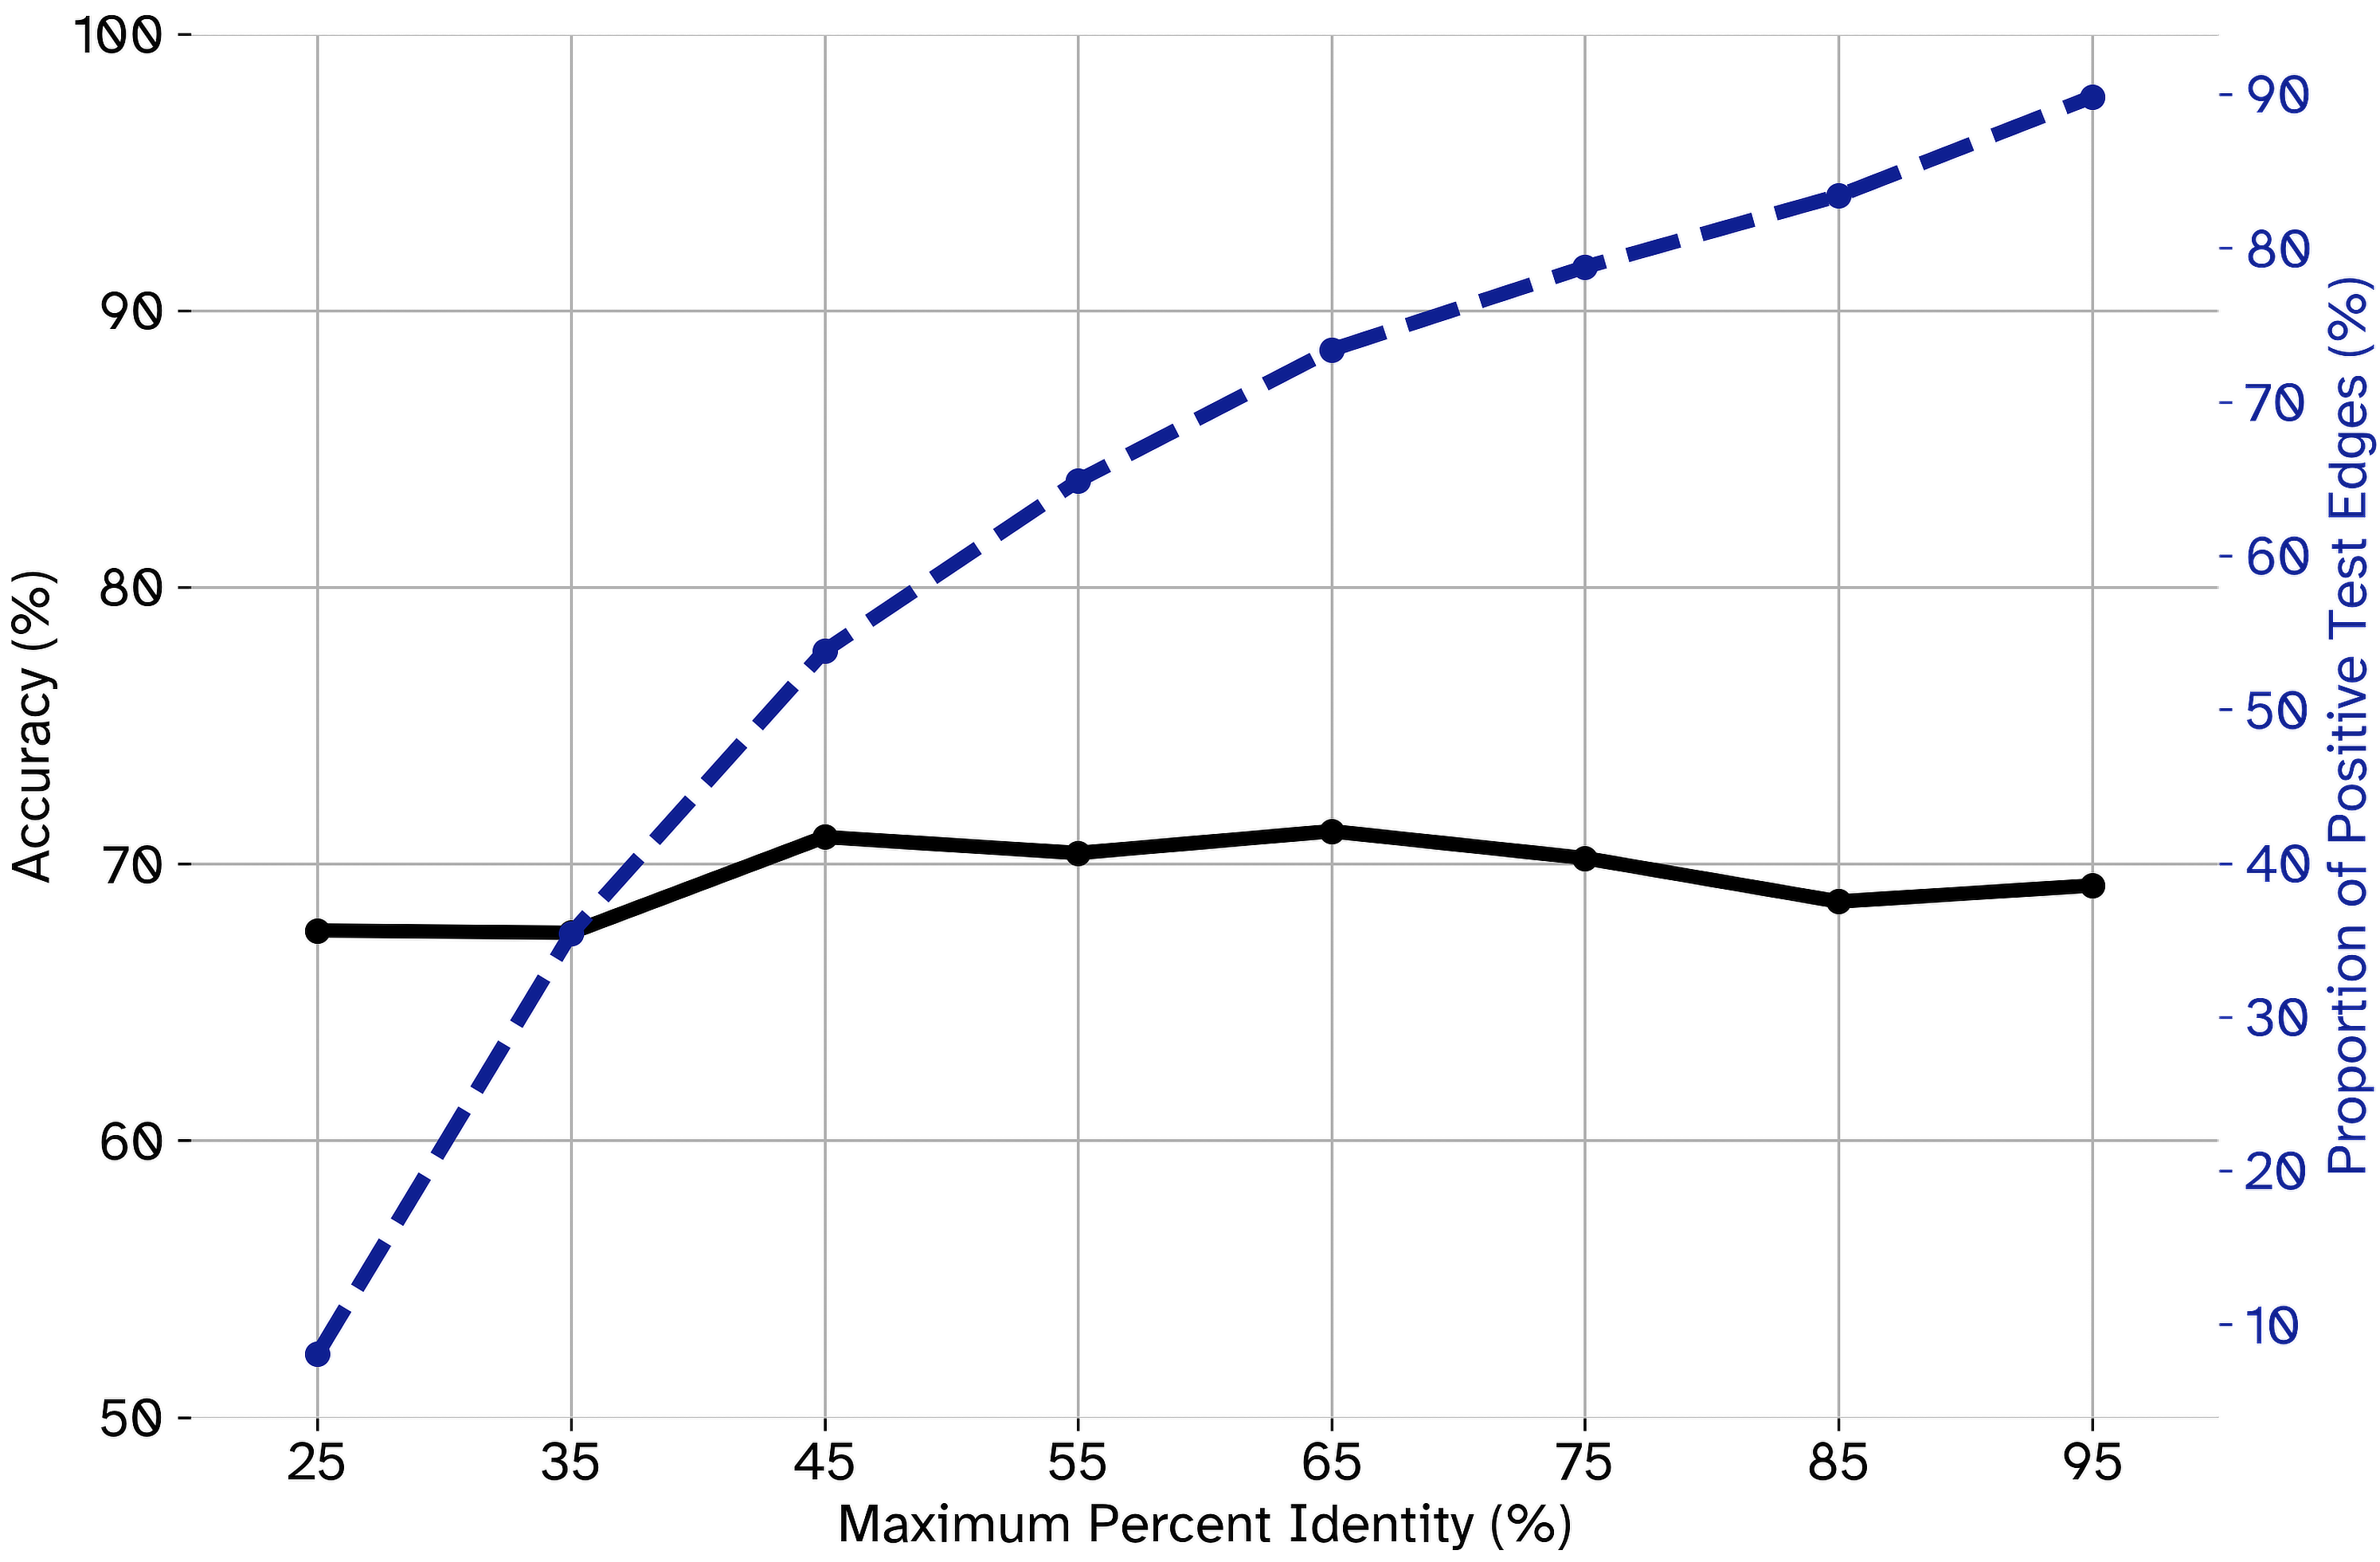
\includegraphics[scale=0.5]{figures/rapppid/perc_id.png}}
	\caption[Accuracy of positive edges as a function of similarity between testing and training proteins in \textsc{c2}.]{\textsf{\textbf{Accuracy of positive edges as a function of similarity between testing and training proteins in C2.}} The similarity between testing and training proteins was measured using their percent identity as computed by \textsc{ncbi}’s \textsc{psi-blast} software. The highest percent identity between any training protein and a testing protein in a testing edge was considered to be that testing edge’s ``maximum percent identity''. The percentage of accurately labelled positive edges (black curve, left y-axis) is reported for edges with maximum percent identities lower than the threshold reported on the x-axis. The proportion of testing edges for each threshold values is reported by the dashed blue curve and the right y-axis.}\label{fig:rapppid:similarity}
\end{figure}

\subsection[Effect of different components on \textsc{rapppid}'s performance]{Effect of different components on RAPPPID's performance}

To understand \textsc{rapppid}’s performance when trained and tested on negative examples which are experimentally validated and manually curated, we created a new C3 dataset where the negative examples are provided by the Negatome database of non-interacting pairs. To combat the large class imbalance caused by the relatively few pairs of human proteins in Negatome (see Section~\ref{sec:rapppid:methods} for details), additional random pair negatives were supplemented until both positive and negative classes had an equal number of samples. After 13 epochs, \textsc{rapppid} achieved a testing \textsc{auroc} of 0.802 and a testing \textsc{aupr} of 0.799 on \textsc{c3} dataset, which is comparable to the performance of \textsc{rapppid} using randomly selected negative edges. Since \textsc{rapppid} utilizes random initialization, mini-batch sampling, and token sampling, there is some stochasticity present in its performance. First, we sought to test the effect of these stochastic components and to ensure that the specific choice of training and test sets were not responsible for the superior performance of \textsc{rapppid}. For this purpose, we ran \textsc{rapppid} twice on three additional \textsc{c3} datasets whose training, validation, and testing proteins were chosen at random (a total of six times). In each of these runs, different seeds were used to assess the effect of stochastic components of \textsc{rapppid} (Supplementary Table \ref{tab:rapppid_repeatability}). Overall, the average testing \textsc{auroc} across models trained on these additional three datasets was 0.792 (60.007). Results from these repeatability experiments illustrate that \textsc{rapppid}’s strong performance on \textsc{c3} datasets is not tied to a specific set of testing or validation proteins, nor certain weight initialization states. Next, we conducted an ablation study (Table~\ref{tab:ablation}) using the same three \textsc{c3} datasets and two runs of each variant per dataset (a total of six models per variant). Each variant substitutes one component of \textsc{rapppid}’s regularization, architecture or optimization, allowing us to quantify the difference in performance for which these components are responsible. In Table 2, `\textsc{rapppid-swa}' variant removes \textsc{swa}, `\textsc{rapppid}+Adam' replaces Ranger21 with Adam optimizer (learning rate selected by hyper-parameter tuning), `\textsc{rapppid-awd}' removes the \textsc{awd} regularization and `\textsc{rapppid}-SentencePiece’ substitutes the SentencePiece tokens with amino-acid-residue-level tokens. As can be seen in Table 2, the choice of optimizer has negligible effect on the performance. However, \textsc{swa}, \textsc{awd}, and SentencePiece tokens all contribute to the superior performance of \textsc{rapppid}, with the tokenizer having the largest contribution. One advantage that SentencePiece affords \textsc{rapppid} is the regularizing effect of random sampling tokens. Additionally, the SentencePiece tokenizer reduces the total length of sequences inputted into the tokenizer. The protein sequences on which \textsc{rapppid} is trained, while limited to 1~500 residues, are sufficiently large enough for gradients to vanish quiet substantially; a phenomenon long known to plague \textsc{rnn}s when trained on long sequences.

\begin{table}[!t]
	\caption[Results from an ablation study conducted on \textsc{rapppid}.]{\textsf{\textbf{Results from an ablation study conducted on RAPPPID.}} \label{tab:ablation}} {\begin{tabular}{@{}lllll@{}}\toprule 
			Experiment & Test \textsc{auroc} & \textsc{auroc} Diff & Testing \textsc{apr} & \textsc{apr} Diff\\\midrule
			\textsc{rapppid} (original) & 0.792 (±0.007) & \textsc{n/a} & 0.794 (±0.009) & \textsc{n/a}\\
			\textsc{rapppid-swa} & 0.782 (±0.007) & -1.20\% & 0.783 (±0.007) & -1.37\%\\
			\textsc{rapppid}+Adam & 0.791 (±0.025) & -0.100\% & 0.792 (±0.032) & -0.273\%\\
			\textsc{rapppid-awd} & 0.762 (±0.020) & -3.70\% & 0.757 (±0.022) & -4.62\%\\
			\textsc{rapppid}-SentencePiece & 0.749 (±0.009) & -5.37\% & 0.748 (±0.011) & -5.85\%\\
			\textsc{rapppid}+TransfLG & 0.670 (±0.030) & -15.3\% & 0.686 (±0.040) & -13.6\%\\
			\textsc{rapppid}+TransfSM & 0.747 (±0.026) & -5.68\% & 0.758 (±0.025) & -4.61\%\\
			\midrule
	\end{tabular}}{}
    \\
    {\footnotesize Note: Each model is trained/tested twice on three randomly generated C3 datasets.\\The performance metrics correspond to held-out test sets.}
\end{table}

In acknowledgement of the recent prevalence and performance of attention-based methods in deep learning (Vaswani \textit{et al.}, 2017), the sixth and seventh variants replace the \textsc{awd-lstm} encoder with transformers of varying sizes. `\textsc{rapppid}+TransfLG' has six layers and eight heads and feed-forward networks with 2048 dimensions, while `\textsc{rapppid}+TransfSM'’ has fewer parameters (2 layers, 2 heads and 80 dimensions). Both transformer variants have a dropout rate of 20\%. The number of heads and layers in \textsc{rapppid}+TransfLG were chosen to closely match those used in the \textsc{bert} language model (Devlin et al., 2019) whose architecture has been previously used for predicting protein function (Elnaggar \textit{et al}., 2021; Rao \textit{et al.}, 2020; Rives \textit{et al.}, 2019). The number of heads and layers for \textsc{rapppid}+TransfSM were chosen to be representative of reasonable lower bounds for those hyperparameters. The results of these analyses (Table 2) reveal that both of these models have worse performance compared to the original \textsc{rapppid} model. The superior performance of the small transformer compared to the large one suggests that the large number of parameters required by transformers are leading to severe overfitting in this task and are the reason behind the performance deterioration.

\subsection{Transfer learning on protein-ligand data from X-ray crystallography experiments}

\textsc{rapppid}'s strong performance on \textsc{c3} datasets demonstrates that it is capable of generalizing to predictions between proteins absent from the training set. Additionally, the ability to generalize these models to make predictions on test datasets that are not representative of the training data (\textit{e.g.} different types of experiments or protocols are used to generate them) is also often desirable, yet is often much more challenging. Transfer learning is one approach that can be used to overcome the challenges imposed by differences between training and test datasets. Transfer learning is the process by which a network is first trained on a large, high-quality dataset. Many of these weights are then `frozen' such that they are no longer backpropagated through, while the remaining `unfrozen' weights are trained on a dataset that is often smaller and/or belongs to a different input distribution (Yosinski \textit{et al.}, 2014). Here, we use this approach to tackle an interaction prediction task on a dataset that differs fundamentally from \textsc{string}: protein-ligand interactions and sequences as determined from X-ray crystallography data. \textsc{string} and similar \textsc{ppi} datasets curate interactions from a wide range of modalities and provide sequences from reference proteomes. We’ve constructed a protein-ligand interaction task by leveraging BioLiP, a semi-manually curated list of X-ray crystallography experiments recorded in the Protein Data Bank (\textsc{pdb}) which reflect interactions between proteins and ligands (Berman \textit{et al.}, 2000; Yang \textit{et al.}, 2013). Using these datasets, we were able to extract sequences from the \textsc{pdb} records and, after filtering out interactions with low-quality sequences, construct a novel protein-ligand dataset. This dataset is available for download through Zenodo at \href{https://doi.org/10.5281/zenodo.6709790}{https://doi.org/10.5281/\\zenodo.6709790} (Szymborski and Emad, 2022a). The sequences extracted from \textsc{pdb} are measured by fundamentally different modalities from those present in \textsc{string}/Uniprot\textsc{kb}, and are often truncated and incomplete as a result. Furthermore, the nature of the interactions recorded by BioLiP is fundamentally different from \textsc{string}. Whereas \textsc{string} catalogues interactions between large classes of proteins, the nature of X-ray crystallography biases captured interactions to those with slower molecular dynamics and which do not primarily exist in aliphatic environments (Carpenter et al., 2008). These fundamental differences between BioLiP and \textsc{string} make them ideal datasets to illustrate the ability to use transfer learning with \textsc{rapppid}. We first pre-trained \textsc{rapppid} on data from \textsc{string}, and then fine-tuned it on the BioLiP dataset after the \textsc{lstm} encoder weights were frozen, leaving only the fully connected classifier to be trained. To ensure no data leakage between the \textsc{string} and BioLiP datasets exists, protein sequences in \textsc{string} determined to have more than 90\% identity with those in BioLiP were moved from the pre-training dataset to the fine-tuning dataset. \textsc{c3}-type training, validation and testing splits were constructed for both the pre-training and finetuning datasets for evaluation purposes. Using this approach, \textsc{rapppid} pre-trained on the \textsc{string} dataset and fine-tuned on a portion of the BioLip dataset achieved an \textsc{auroc} of 0.909. To test our hypothesis that transfer learning is indeed necessary to achieve good performance on this dataset, we also directly applied the pretrained \textsc{rapppid} model (without any fine-tuning on BioLip) to the BioLip test split. As expected, this resulted in almost random results (\textsc{auroc} = 0.548). These results highlight the difficulties of generalizing a model to fundamentally different datasets and emphasise the utility of transfer learning to achieve good performance using \textsc{rapppid} in such scenarios.

\subsection[\textsc{rapppid} predicts interaction of \textsc{her2} with Trastuzumab and\\Pertuzumab]{RAPPPID predicts interaction of HER2 with Trastuzumab and\\Pertuzumab}

Peptides and proteins have emerged as an important class of therapeutics, enabling researchers to target previously `undruggable' targets (Tsomaia, 2015). Hundreds of peptide and protein therapeutics have been approved by the \textsc{u.s.} Food and Drug Administration (Usmani \textit{et al.}, 2017) with applications in treating illnesses ranging from cancer to heart disease (Chen \textit{et al.}, 2012; Sikder \textit{et al.}, 2019). Here, we sought to illustrate how one might use \textsc{rapppid} to validate hypothesized interactions between target proteins and candidate therapeutic proteins and peptides through two examples: Trastuzumab and Pertuzumab. Trastuzumab and Pertuzumab are two recombinant humanized monoclonal antibodies which are used in combination in the treatment of metastatic breast cancers which belong to the \textsc{her2}-positive subtype (Boekhout \textit{et al.}, 2011; Malenfant \textit{et al.}, 2014). Both Trastuzumab and Pertuzumab target distinct domains of the human epidermal growth factor receptor 2 (\textsc{her2}). We applied \textsc{rapppid}, trained on our \textit{H.~sapiens} \textsc{string} \textsc{c2} dataset (which is more appropriate for this application), to the sequences of the Trastuzumab and Pertuzumab antibody chains. \textsc{rapppid} predicted that \textsc{her2} interacts with Trastuzumab and Pertuzumab with 98.8\% and 95.1\% probability, respectively. When compared to the interaction probabilities between these drugs and all other proteins in the \textsc{string} database, these probabilities are within the first and second percentile for Trastuzumab and Pertuzumab, respectively (Supplementary Fig. \ref{fig:rapppid:trastuzumab}). In addition, the majority of proteins are predicted to have a probability of interacting with Trastuzumab and Pertuzumab of 35.9\% and 28.8\%, respectively.

\section{Discussion}

This study introduced \textsc{rapppid}, a deep learning method that addresses the challenges of creating generalizable \textsc{ppi} prediction models posed by inherent characteristics of \textsc{ppi} datasets. By adopting a modified \textsc{awd-lstm} training routine, \textsc{rapppid} was able to surpass state-of-the-art models under testing conditions that carefully controlled for information leakage and other sources of prediction accuracy inflation. Further experiments were conducted to confirm the results were independent of the specific proteins present in the training and testing splits. \textsc{rapppid}s ability to \textsc{ppi}s in the \textsc{string} database was shown to increase with strong biological evidence for the interaction. This relationship between \textsc{ppi} evidence and \textsc{rapppid} predictive ability illustrates that \textsc{rapppid} accurately reflects our confidence in interactions, and testing performance is not disproportionately inflated by spurious, low-confidence interactions. Moreover, assessment of the sequence similarity between testing and training proteins revealed that the superior performance of \textsc{rapppid} is not due to the presence of highly similar protein pairs in testing and training, and the accuracy of \textsc{rapppid} was largely stable with a small improvement when highly similar testing proteins were excluded. Developing appropriate and meaningful benchmark datasets for \textsc{ppi} prediction remains a challenging problem for a number of reasons. First, deep learning tasks rely on large, high-quality datasets to obtain meaningful generalized models. Such datasets are few and far between. Projects like \textsc{hippie} and iRefWeb join \textsc{string} in being among the best examples of \textsc{ppi} datasets which integrate multiple sources to assure both quality and quantity of \textsc{ppi} edges (Alanis-Lobato \textit{et al.}, 2017; Turner \textit{et al.}, 2010). Despite this, \textsc{string} is the only dataset among these three which has an appropriate number of high-confidence edges for the purpose of learning deep learning model. Specifically, there are 98.5\% fewer edges in \textsc{hippie} than in \textsc{string} between human proteins at a 95\% confidence threshold. Even when confidence thresholds are lowered to 85\%, \textsc{hippie} holds 87.9\% fewer human edges than \textsc{string}. Similarly, \textsc{string} at a 95\% confidence threshold has 75\% more human edges when considering iRefWeb edges with three supporting references or more. Second, this reliance on large, representative datasets is further exacerbated by the unique overfitting challenges posed by the characteristics of \textsc{ppi} data, as explored in this work and in Park and Marcotte (Park and Marcotte, 2012). While \textsc{rapppid} mitigates the overfitting tendencies of \textsc{ppi} data through regularization, it also relies on large, representative training data to do so. In the construction of our \textsc{c3} datasets, it is necessary to discard edges which are not between proteins of the same validation split. As a result, we observe a further decrease of up to 33.9\% in the number of the already-precious-few edges afforded to us by \textsc{string}. As we have shown in this work, the construction of benchmark datasets is critical for effectively comparing and evaluating \textsc{ppi} prediction tasks. It is thanks to large, quality \textsc{ppi} dataset projects like \textsc{string} that we might construct meaningful and appropriate datasets against which to evaluate \textsc{ppi} prediction methods like \textsc{rapppid}. Additional efforts and methodologies to collect and integrate \textsc{ppi} edges of the scale of \textsc{string} at high confidence levels are greatly desired, as they can help identify and mitigate biases that inevitably arise when constructing datasets. In our analysis, we observed that \textsc{rapppid} assigns a very high probability of interaction to \textsc{her2} and Trastuzumab (first percentile) and Pertuzumab (second percentile). In spite of this, there are still proteins that are predicted by \textsc{rapppid} to interact with these two antibodies with similar or higher probabilities (72 for Trastuzumab and 206 for Pertuzumab). This of course is not unique to \textsc{rapppid} and other methods also face this issue to an even a greater extent. For example, \textsc{sprint} (the second-best performing algorithm after \textsc{rapppid}) assigns a higher interaction score to 389 proteins for Trastuzumab-\textsc{her2} and 456 proteins for Pertuzumab-\textsc{her2}. We believe there are several factors contributing to this. First, all of these methods face some limitations in their performance, as we explored and observed in our cross-validation analyses. Second, there are off-target effects of these antibodies that make the prediction challenging for these computational models. Finally, there may be domain shifts between the interacting proteins in \textsc{string} dataset and the interaction of these antibodies and their targets, a similar phenomenon that we observed in BioLiP dataset. This suggests that transfer learning approaches such as the one we used for BioLiP dataset may be useful to improve the specificity of these algorithms, a direction that we will pursue in the future. As a result of these factors, while \textsc{rapppid} can be used to narrow down the search space of novel therapeutic antibodies and peptides, it does not remove the necessity of follow-up experimental validations to identify their targets. The task of \textsc{ppi} prediction is related to the problem of protein docking inference, whereby computational models predict the atomic interactions between two proteins. While many methods have historically been based on the fast Fourier transform for energy evaluation (Desta \textit{et al.}, 2020), new and effective deep learning methods have also become available. One such method is AlphaFold-multimer (Evans \textit{et al.}, 2021), which builds upon an attention-based model for the prediction of protein structure (Jumper \textit{et al.}, 2021) to infer the interface of homo and hetero protein dimers at an atomic level. Integrating docking predictions can be an interesting future direction to help improve \textsc{rapppid}’s \textsc{ppi} prediction generalization. \textsc{rapppid}’s ability to predict interactions warrants further study into relevant tasks that might benefit from a similar approach. The \textsc{rapppid} architecture might be modified for the tasks of binding site and protein function prediction. These tasks are related to \textsc{ppi} prediction and as a result are exposed to similar challenges to which \textsc{rapppid} is well suited. While our ablation studies found that \textsc{rapppid} using a Transformer architecture for the encoder performed worse than an \textsc{awd-lstm}, using a Transformer model pre-trained on amino acid sequences might improve performance. However, in all these cases, it is crucial to consider strict rules for cross-validation and data splitting to ensure data leakage is avoided.

\section*{Authors' contributions}
\addcontentsline{toc}{section}{Authors' contributions}

\textsc{a.e.} and \textsc{j.s.} conceived the study, designed the project and the algorithm, and wrote the article. \textsc{j.s.} implemented the pipeline and performed the statistical analyses of the results. All authors read and approved the final article.

\section*{Funding}
\addcontentsline{toc}{section}{Funding}

This work was supported by the Natural Sciences and Engineering Research Council of Canada (\textsc{nserc}) grant [\textsc{rgpin}-2019-04460 to \textsc{a.e.}] and by the McGill Initiative in Computational Medicine (MiCM) (to \textsc{a.e.}). This research was enabled in part by support provided by Calcul Qu\'ebec (\href{https://www.calculquebec.ca/}{www.calculquebec.ca}) and Compute Canada (\href{https://www.computecanada.ca}{www.computecanada.ca}).

\section*{Data availability}
\addcontentsline{toc}{section}{Data availability}

The data underlying this article are available on Zenodo.org, at \href{https://doi.org/10.5281/zenodo.6709790}{https://doi.org/10.5281/zenodo.\\6709790}.

\begin{singlespace}
\def\bibindent{1em}
\makeatletter
\renewcommand{\thebibliography}[1]{%
  \section*{\bibname}%
  \addcontentsline{toc}{section}{References}
  \@mkboth{\MakeUppercase\bibname}{\MakeUppercase\bibname}%
  \list{\@biblabel{\@arabic\c@enumiv}}%
       {\settowidth\labelwidth{\@biblabel{#1}}%
        \leftmargin\labelwidth
        \advance\leftmargin\labelsep
        \@openbib@code
        \usecounter{enumiv}%
        \let\p@enumiv\@empty
        \renewcommand\theenumiv{\@arabic\c@enumiv}}%
  \sloppy
  \clubpenalty4000
  \@clubpenalty \clubpenalty
  \widowpenalty4000%
  \sfcode`\.\@m}
\makeatother
\renewcommand{\bibname}{References}
\begin{thebibliography}{99\kern\bibindent}
\markboth{Chapter 3: \textsc{rapppid}}{Chapter 3: \textsc{rapppid}}
\makeatletter
\def\@biblabel#1{}
\let\old@bibitem\bibitem
\def\bibitem#1{\old@bibitem{#1}\leavevmode\kern-\bibindent}
\makeatother
\bibitem{Lorem}Alanis-Lobato,G. \textit{et al.} (2017) Hippie v2.0: enhancing meaningfulness and reliability of protein–protein interaction networks. \textit{Nucleic Acids Res.}, 45, D408–D414.
\bibitem{Lorem}Altschul,S.F. \textit{et al.} (1990) Basic local alignment search tool. \textit{J. Mol. Biol.}, 215, 403–410.
\bibitem{Lorem}Altschul,S.F. \textit{et al.} (1997) Gapped BLAST and PSI-BLAST: a new generation of protein database search programs. \textit{Nucleic Acids Res.}, 25, 3389–3402.
\bibitem{Lorem}Anfinsen,C.B. (1973) Principles that govern the folding of protein chains. \textit{Science}, 181, 223–230.
\bibitem{Lorem}Athiwaratkun,B. \textit{et al.} (2019) There are many consistent explanations of unlabeled data: Why you should average. In: \textit{7th International Conference on Learning Representations, ICLR 2019, New Orleans, LA, USA, May 6-9, 2019}. OpenReview.net.
\bibitem{Lorem}Ben-Hur,A. and Noble,W.S. (2005) Kernel methods for predicting protein-protein interactions. \textit{Bioinformatics}, 21, i38–i46.
\bibitem{Lorem}Ben-Hur,A. and Noble,W.S. (2006) Choosing negative examples for the prediction of protein-protein interactions. \textit{BMC Bioinformatics}, 7, S2.
\bibitem{Lorem}Berman,H.M. \textit{et al.} (2000) The protein data bank. \textit{Nucleic Acids Res.}, 28, 235–242.
\bibitem{Lorem}Blohm,P. \textit{et al.} (2014) Negatome 2.0: a database of non-interacting proteins derived by literature mining, manual annotation and protein structure analysis. \textit{Nucleic Acids Res.}, 42, D396–D400.
\bibitem{Lorem}Boekhout,A.H. \textit{et al.} (2011) Trastuzumab. \textit{Oncologist}, 16, 800–810.
\bibitem{Lorem}Brock,A. \textit{et al.} (2021) High-performance large-scale image recognition without normalization. arXiv:2102.06171 [cs, stat]. arXiv: 2102.06171. https: //doi.org/10.48550/arXiv.2102.06171.
\bibitem{Lorem}Bromley,J. \textit{et al.} (1993) Signature verification using a ``Siamese'' time delay neural network. \textit{Int. J. Pattern Recognit. Artif. Intell.}, 07, 669–688.  
\bibitem{Lorem}Browne,F. \textit{et al.} (2007) Supervised statistical and machine learning approaches to inferring pairwise and module-based protein interaction networks. In: \textit{2007 IEEE 7th International Symposium on BioInformatics and BioEngineering}. IEEE, Boston, MA, USA, pp. 1365–1369. 
\bibitem{Lorem}Carpenter,E.P. \textit{et al.} (2008) Overcoming the challenges of membrane protein crystallography. \textit{Curr. Opin. Struct. Biol.}, 18, 581–586. 
\bibitem{Lorem}Chen,H.H. \textit{et al.} (2012) Novel protein therapeutics for systolic heart failure: chronic subcutaneous b-type natriuretic peptide. \textit{J. Am. Coll. Cardiol.}, 60, 2305–2312. 
\bibitem{Lorem}Chen,M. \textit{et al.} (2019) Multifaceted protein–protein interaction prediction based on Siamese residual RCNN. \textit{Bioinformatics}, 35, i305–i314. 
\bibitem{Lorem}Cong,Q. \textit{et al.} (2019) Protein interaction networks revealed by proteome coevolution. \textit{Science}, 365, 185–189. 
\bibitem{Lorem}Desta,I.T. \textit{et al.} (2020) Performance and its limits in rigid body protein-protein docking. \textit{Structure}, 28, 1071–1081.e3. 
\bibitem{Lorem}Devlin,J. \textit{et al.} (2019) Bert: Pre-training of deep bidirectional transformers for language understanding. arXiv:1810.04805 [cs]. arXiv: 1810.04805. https: //doi.org/10.48550/arXiv.1810.04805. 
\bibitem{Lorem}Dick,K. \textit{et al.} (2020) Pipe4: Fast PPI predictor for comprehensive inter- and cross-species interactomes. \textit{Sci. Rep.}, 10, 1390. 
\bibitem{Lorem}Ding,Y. \textit{et al.} (2016) Predicting protein-protein interactions via multivariate mutual information of protein sequences. \textit{BMC Bioinformatics}., 17, 398. 
\bibitem{Lorem}Elnaggar,A. \textit{et al.} (2021) ProtTrans: towards cracking the language of life’s code through self-supervised learning. page 2020.07.12.199554. https: //doi.org/10.1101/2020.07.12.199554. 
\bibitem{Lorem}Evans,R. \textit{et al.} (2021) Protein complex prediction with AlphaFold-multimer. https://doi.org/10.1101/2021.10.04.463034.  
\bibitem{Lorem}Falcon,W. \textit{et al.} (2020) PyTorchLightning/Pytorch-Lightning: 0.7.6 Release. Zenodo. https://doi.org/10.5281/ZENODO.3828935. 
\bibitem{Lorem}Gillis,J. \textit{et al.} (2014) Bias tradeoffs in the creation and analysis of protein–protein interaction networks. \textit{J. Proteomics}, 100, 44–54. 
\bibitem{Lorem}Henikoff,S. and Henikoff,J.G. (1992) Amino acid substitution matrices from protein blocks. \textit{Proc. Natl. Acad. Sci.} USA, 89, 10915–10919. 
\bibitem{Lorem}Hochreiter,S. and Schmidhuber,J. (1997) Long short-term memory. \textit{Neural Comput.}, 9, 1735–1780. 
\bibitem{Lorem}Huttlin,E.L. \textit{et al.} (2017) Architecture of the human interactome defines protein communities and disease networks. \textit{Nature}, 545, 505–509. 
\bibitem{Lorem}Izmailov,P. \textit{et al.} (2019) Averaging weights leads to wider optima and better generalization. arXiv:1803.05407 [cs, stat]. arXiv: 1803.05407. https: //doi.org/10.48550/arXiv.1803.05407.
\bibitem{Lorem}Jansen,R. \textit{et al.} (2003) A Bayesian networks approach for predicting protein-protein interactions from genomic data. \textit{Science}, 302, 449–453. 
\bibitem{Lorem}Jassal,B. \textit{et al.} (2020) The Reactome pathway knowledgebase. \textit{Nucleic Acids Res.}, 48, D498–D503. 
\bibitem{Lorem}Jumper,J. \textit{et al.} (2021) Highly accurate protein structure prediction with AlphaFold. \textit{Nature}, 596, 583–589. 
\bibitem{Lorem}Kanehisa,M. and Goto,S. (2000) KEGG: Kyoto Encyclopedia of genes and genomes. \textit{Nucleic Acids Res.}, 28, 27–30. 
\bibitem{Lorem}Kudo,T. (2018) Subword regularization: Improving neural network translation models with multiple subword candidates. arXiv:1804.10959 [cs]. arXiv: 1804.10959. https://doi.org/10.48550/arXiv.1804.10959. 
\bibitem{Lorem}Kudo,T. and Richardson,J. (2018) Sentencepiece: a simple and language independent subword tokenizer and detokenizer for neural text processing. In: \textit{Proceedings of the 2018 Conference on Empirical Methods in Natural Language Processing: System Demonstrations. Association for Computational Linguistics}, Brussels, Belgium, pp. 66–71. 
\bibitem{Lorem}Li,Y. and Ilie,L. (2017) Sprint: ultrafast protein-protein interaction prediction of the entire human interactome. \textit{BMC Bioinformatics}, 18, 485. 
\bibitem{Lorem}Lipton,Z.C. \textit{et al.} (2015) A critical review of recurrent neural networks for sequence learning. arXiv:1506.00019 [cs]. arXiv: 1506.00019. https: //doi.org/10.48550/arXiv.1506.00019. 
\bibitem{Lorem}Loshchilov,I. and Hutter,F. (2019) Decoupled weight decay regularization. In: \textit{7th International Conference on Learning Representations, ICLR 2019}, New Orleans, LA, USA, May 6-9, 2019. OpenReview.net.  
\bibitem{Lorem}Malenfant,S.J. \textit{et al.} (2014) Pertuzumab: a new targeted therapy for her2-positive metastatic breast cancer. \textit{Pharmacotherapy}, 34, 60–71. 
\bibitem{Lorem}Merity,S. \textit{et al.} (2017) Regularizing and optimizing LSTM language models. arXiv:1708.02182 [cs]. arXiv: 1708.02182. https://doi.org/10. 48550/arXiv.1708.02182. 
\bibitem{Lorem}Misra,D. (2020) Mish: a self-regularized non-monotonic activation function. arXiv:1908.08681 [cs, stat]. arXiv: 1908.08681. https://doi.org/ 10.48550/arXiv.1908.08681. 
\bibitem{Lorem}Orchard,S. \textit{et al.} (2012) Protein interaction data curation: the international molecular exchange (IMEx) consortium. \textit{Nat. Methods}, 9, 345–350. 
\bibitem{Lorem}Orchard,S. \textit{et al.} (2014) The MIntAct project—IntAct as a common curation platform for 11 molecular interaction databases. \textit{Nucleic Acids Res.}, 42, D358–D363. 
\bibitem{Lorem}Oughtred,R. \textit{et al.} (2021) The BioGRID database: a comprehensive biomedical resource of curated protein, genetic, and chemical interactions. \textit{Protein Sci.}, 30, 187–200. 
\bibitem{Lorem}Park,Y. and Marcotte,E.M. (2012) Flaws in evaluation schemes for pair-input computational predictions. \textit{Nat. Methods}, 9, 1134–1136. 
\bibitem{Lorem}Paszke,A. \textit{et al.} (2019) Pytorch: an imperative style, high-performance deep learning library. In: Wallach,H.M. \textit{et al.} (eds), \textit{Advances in Neural Information Processing Systems 32: Annual Conference on Neural Information Processing Systems 2019, NeurIPS 2019}, 8-14 December 2019, Vancouver, BC, Canada, pp. 8024–8035.  
\bibitem{Lorem}Rao,R. \textit{et al.} (2020) Transformer protein language models are unsupervised structure learners. bioRxiv, 2020.12.15.422761. https://doi.org/10. 1101/2020.12.15.422761. 
\bibitem{Lorem}Richoux,F. \textit{et al.} (2019) Comparing two deep learning sequence-based models for protein-protein interaction prediction. arXiv:1901.06268 [cs, q-bio, stat]. arXiv: 1901.06268. https://doi.org/10.48550/arXiv.1901.06268. 
\bibitem{Lorem}Rives,A. \textit{et al.} (2019) Biological structure and function emerge from scaling unsupervised learning to 250 million protein sequences. bioRxiv, 622803. https://doi.org/10.1101/622803. 
\bibitem{Lorem}Roux,K.J. \textit{et al.} (2012) A promiscuous biotin ligase fusion protein identifies proximal and interacting proteins in mammalian cells. \textit{J. Cell Biol.}, 196, 801–810. 
\bibitem{Lorem}Salwinski,L. \textit{et al.} (2004) The database of interacting proteins: 2004 update. \textit{Nucleic Acids Res.}, 32, D449–451.
\bibitem{Lorem}Schuster,M. and Nakajima,K. (2012) Japanese and Korean voice search. In: \textit{2012 IEEE International Conference on Acoustics, Speech and Signal Processing, ICASSP 2012}, Kyoto, Japan, March 25-30, 2012. IEEE, pp. 5149–5152. 
\bibitem{Lorem}Sikder,S. \textit{et al.} (2019) Long-term delivery of protein and peptide therapeutics for cancer therapies. \textit{Exp. Opin. Drug Deliv.}, 16, 1113–1131. 
\bibitem{Lorem}Snider,J. \textit{et al.} (2015) Fundamentals of protein interaction network mapping. \textit{Mol. Syst. Biol.}, 11, 848.  
\bibitem{Lorem}Srivastava,N. \textit{et al.} (2014) Dropout: a simple way to prevent neural networks from overfitting. \textit{J. Mach. Learn. Res.}, 15, 1929–1958. 
\bibitem{Lorem}Szklarczyk,D. \textit{et al.} (2019) String v11: protein–protein association networks with increased coverage, supporting functional discovery in genome-wide experimental datasets. \textit{Nucleic Acids Res.}, 47, D607–D613. 
\bibitem{Lorem}Szymborski,J. and Emad,A. (2022a) Data for RAPPPID: towards generalisable protein interaction prediction with AWD-LSTM Twin Networks. https: //doi.org/10.5281/zenodo.6709790. 
\bibitem{Lorem}Szymborski,J. and Emad,A. (2022b) Software for RAPPPID: regularised automative prediction of protein-protein interactions using Deep Learning. https://doi.org/10.5281/zenodo.6709213. 
\bibitem{Lorem}Tabe-Bordbar,S. \textit{et al.} (2018) A closer look at cross-validation for assessing the accuracy of gene regulatory networks and models. \textit{Sci. Rep.}, 8, 6620. 
\bibitem{Lorem}Tsomaia,N. (2015) Peptide therapeutics: targeting the undruggable space. \textit{Eur. J. Med. Chem.}, 94, 459–470.  
\bibitem{Lorem}Turner,B. \textit{et al.} (2010) iRefWeb: interactive analysis of consolidated protein interaction data and their supporting evidence. \textit{Database (Oxford)}, 2010, baq023. 
\bibitem{Lorem}Usmani,S. \textit{et al.} (2017) THPdb: database of FDA-approved peptide and protein therapeutics. \textit{PLoS One}, 12, e0181748. 
\bibitem{Lorem}Vaswani, A. \textit{et al.} (2017) Attention is all you need. In: \textit{Proceedings of the 31st International Conference on Neural Information Processing Systems, NIPS’17}. Curran Associates Inc., Red Hook, NY, USA, pp. 6000–6010. 
\bibitem{Lorem}Vidal,M. and Fields,S. (2014) The yeast two-hybrid assay: still finding connections after 25 years. \textit{Nat. Methods}, 11, 1203–1206. 
\bibitem{Lorem}Wan,L. \textit{et al.} (2013) Regularization of neural networks using DropConnect. In: Dasgupta, S. and McAllester, D. (eds). \textit{Proceedings of the 30th International Conference on Machine Learning, Volume 28 of Proceedings of Machine Learning Research. PMLR}, Atlanta, GA, USA, pp. 1058–1066. 
\bibitem{Lorem}Wright,L. and Demeure,N. (2021) Ranger21: a synergistic deep learning optimizer. arXiv:2106.13731 [cs]. arXiv: 2106.13731. https://doi.org/ 10.48550/arXiv.2106.13731. 
\bibitem{Lorem}Yang,J. \textit{et al.} (2013) BioLip: a semi-manually curated database for biologically relevant ligand–protein interactions. \textit{Nucleic Acids Res.}, 41, D1096–D1103. 
\bibitem{Lorem}Yong,H. \textit{et al.} (2020) Gradient centralization: a new optimization technique for deep neural networks. In: Vedaldi,A. \textit{et al.} (eds), \textit{Computer Vision ECCV 2020 - 16th European Conference}, Glasgow, UK, August 23-28, 2020, Proceedings, Part I, Lecture Notes in Computer Science. Springer, pp. 635–652.  
\bibitem{Lorem}Yosinski,J. \textit{et al.} (2014) How Transferable Are Features in Deep Neural Networks? In: Ghahramani,Z. \textit{et al.} (eds), \textit{Advances in Neural Information Processing Systems 27: Annual Conference on Neural Information Processing Systems} 2014, December 8-13 2014, Montr\'eal, Qu\'ebec, Canada, pp. 3320–3328. 
\bibitem{Lorem}Zaremba,W. \textit{et al.} (2015) Recurrent neural network regularization. arXiv: 1409.2329 [cs]. arXiv: 1409.2329. https://doi.org/10.48550/arXiv.1409. 2329. 
\bibitem{Lorem}Zhang,M.R. \textit{et al.} (2019) Lookahead optimizer: k steps forward, 1 step back. In: Wallach,H.M. \textit{et al.} (eds), \textit{Advances in Neural Information Processing Systems 32: Annual Conference on Neural Information Processing Systems 2019, NeurIPS} 2019, 8-14 December 2019, Vancouver, BC, Canada, pp. 9593–9604.
\end{thebibliography}
\end{singlespace}
  \begin{singlespace}
\chapter*{Background and Context for ``\textit{Causal single-cell RNA-seq simulation, in silico perturbation, and GRN inference benchmarking using GRouNdGAN-Toolkit}''}
\markboth{Background and Context for \textsc{GRouNdGAN-Toolkit}}{Background and Context for \textsc{GRouNdGAN-Toolkit}}
\end{singlespace}

While \textsc{rapppid} represented a meaningful advance in our ability to make accurate predictions on datasets which controlled for data leakage, generalization remained (and continues to remain) a challenge for \textsc{ppi} inference models. Following the publication of \textsc{rapppid}, we began to look to specific areas in which \textsc{ppi} inference models fail to generalize. Predicting interactions between proteins of different organism, particularly those of very evolutionary distance species, had been previously identified as a challenge for \textsc{ppi} inference models \cite{dick_pipe4_2020, sledzieski_d-script_2021}. What's more, these ``cross-species'' interactions are of great value to researchers. The vast majority of \textsc{ppi}s studied belong to a small number of model organisms representing a small fraction of all species, representing less than a third of taxa at the class rank as measured by the \textsc{string} core dataset \cite{intrepppid}. We've named this discrepancy in elucidated \textsc{ppi}'s the ``species gap''. It follows, then, that it would be greatly advantageous to construct computational methods for expanding our knowledge of \textsc{ppi}s in species other than a select few model organisms.

The cross-species \textsc{ppi} inference models of which I was aware at the time, however, conducted their evaluations on datasets which suffered from data leakage \cite{dick_pipe4_2020, sledzieski_d-script_2021}. Further, when evaluated on a strict, \textsc{c3} dataset which controlled for data leakage, performance severely deteriorated \cite{intrepppid}.

This is the context from which our method \textsc{intrepppid} arose \cite{intrepppid}. \textsc{intrepppid} builds upon the lessons and architecture of \textsc{rapppid}, leaving unchanged its \textsc{awd-lstm} encoder, expanding the model such that it now also modelled the orthology between proteins. Orthology here can be thought of similarities in protein sequence across species due them sharing a common ancestor \cite{fang_getting_2010}. Modelling orthology proved to have many synergistic effects with the cross-species task, lending itself particularly well to both theoretical and practical concerns. Theoretically, homology is a natural place to begin when comparing the interactions of two species, and forms the basis of many early analyses such as Date and Marcotte's work as well as that of Sharan \textit{et al.} \cite{date_discovery_2003, sharan_conserved_2005}. Practically, the orthology modelling task can be argued to provide a regularizing effect when viewed through the lens of contrastive self-supervised learning \cite{intrepppid, chen_simple_2020, sermanet_time-contrastive_2018}. Due to our novel ``quintuplet'' architecture, whereby an encoders weights are shared across a twin network task as well as as a triplet contrastive network, the number of parameters used in the \textsc{intrepppid} network were ostensibly identical to that of \textsc{rapppid}. 

\textsc{intrepppid} successfully improved on \textsc{rapppid}'s predictive performance on testing pairs between proteins of the same  and differing organisms \cite{intrepppid}. Experiments also demonstrated that the improvements in predictive performance that \textsc{intrepppid} enjoyed were due to having successfully modelled orthology, rather than any spurious or unintended cause resulting from the novel ``quintuplet'' architecture. \textsc{intrepppid}'s efficient architecture and resulting low computational requirements has allowed us to create an online service, \href{https://ppi.bio}{\textsc{ppi}.bio}, for using \textsc{intrepppid} and \textsc{rapppid} to infer \textsc{ppi} interactions. Together, the work presented in the \textsc{intrepppid} manuscript represent a concrete step in the direction of narrowing the species gap.

%\textsc{intrepppid} demonstrates a novel network construction which was designed with a focus on its ability to model the underlying biological data while using regularization techniques and a limited number of parameters to account for the limited amount of high-quality \textsc{ppi} training pairs are available to us. Together with the tools we've created to make \textsc{ppi} inference more accessible with \href{https://ppi.bio}{\textsc{ppi}.bio}, the work presented in the \textsc{intrepppid} manuscript brings us closer to narrowing the species gap.

\begin{tcolorbox}
    The contents of Chapter 4 were first published on the 22\textsuperscript{nd} of August, 2024 as an article of the same title in Volume 25, Issue 5, of Oxford University Press' \textit{Briefings in Bioinformatics} journal and is made available under the \href{https://creativecommons.org/licenses/by-nc/4.0/legalcode.en}{Creative Commons Attribution-NonCommercial License}, © Joseph Szymborski and Amin Emad, 2024. \textsc{doi}: \href{https://doi.org/10.1093/bib/bbae405}{10.1093/bib/bbae405}
\end{tcolorbox}

\begin{singlespace}
\chapter[Causal single-cell RNA-seq simulation, in silico perturbation, and GRN inference benchmarking using GRouNdGAN-Toolkit]{Causal single-cell RNA-seq simulation, in silico perturbation, and GRN inference benchmarking using GRouNdGAN-Toolkit}
\markboth{Chapter 4: GRouNdGAN-Toolkit}{Chapter 4: GRouNdGAN-Toolkit}%
\end{singlespace}

\counterwithout{section}{chapter}
\renewcommand{\thetable}{\arabic{table}}
\renewcommand{\thefigure}{\arabic{figure}}

\figuresection{Causal single-cell RNA-seq simulation, in silico perturbation, and GRN inference benchmarking using GRouNdGAN-Toolkit}

\section*{Abstract}
\addcontentsline{toc}{section}{Abstract}
An overwhelming majority of protein–protein interaction (\textsc{ppi}) studies are conducted in a select few model organisms largely due to constraints in time and cost of the associated ‘wet lab’ experiments. In silico \textsc{ppi} inference methods are ideal tools to overcome these limitations, but often struggle with cross-species predictions. We present \textsc{intrepppid}, a method that incorporates orthology data using a new ‘quintuplet’ neural network, which is constructed with five parallel encoders with shared parameters. \textsc{intrepppid} incorporates both a \textsc{ppi} classification task and an orthologous locality task. The latter learns embeddings of orthologues that have small Euclidean distances between them and large distances between embeddings of all other proteins. \textsc{intrepppid} outperforms all other leading \textsc{ppi} inference methods tested on both the intraspecies and cross-species tasks using strict evaluation datasets. We show that \textsc{intrepppid}’s orthologous locality loss increases performance because of the biological relevance of the orthologue data and not due to some other specious aspect of the architecture. Finally, we introduce \textsc{ppi}.bio and \textsc{ppi} Origami, a web server interface for \textsc{intrepppid} and a software tool for creating strict evaluation datasets, respectively. Together, these two initiatives aim to make both the use and development of \textsc{ppi} inference tools more accessible to the community.
\newpage
\section*{Graphical Abstract}

\begin{figure}[h]%figure2
	\centerline{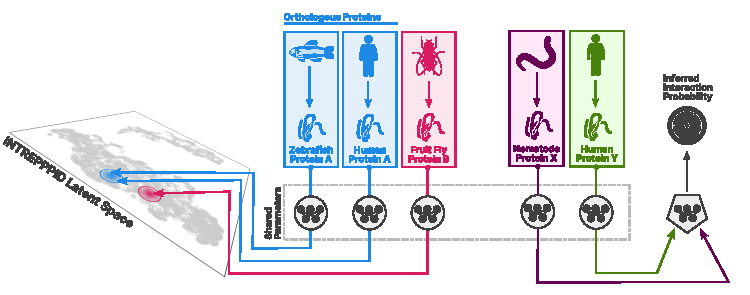
\includegraphics[scale=1]{figures/intrepppid/graphical_abstract.pdf}}
\end{figure}

\textbf{Keywords}: protein-protein interactions; orthology; cross-species; deep learning

\section*{Introduction}
\addcontentsline{toc}{section}{Introduction}
Studying how proteins work in concert has yielded deeply valuable biological insights. Not least of these insights is the implication of protein interactions in the appearance of biological phenotypes and relatedly, how disrupting these interactions can lead to disease [1, 2]. Knowledge of these interactions can, in turn, be used to design drugs and therapies to treat the diseases for which they are implicated [3, 4].

As the relevant technologies have improved, studies which experimentally verify protein–protein interactions (\textsc{ppi}s) have increased in size. In fact, multiple recent studies have published so-called `all-by-all' studies whereby the interaction of entire proteomes are experimentally evaluated. In September 2014, researchers assembled a reference network of ∼14~000 interactions from a search space of 13~000 human genes through a combination of yeast-two-hybrid (\textsc{y2h}) assays and other validation experiments [5]. Five years later, the same network (‘\textsc{h}u\textsc{ri}’) expanded to ∼53~000 interactions from a search space of 17~500 proteins [6].

While these studies provide an invaluable wealth of data, they represent a tremendous investment of time, labour, and money. A major consequence of the high cost of `all-by-all' studies is that it is prohibitively expensive to exhaustively perform them for all known species. In fact, it is currently only practical to limit these studies to a small number of well-studied model organisms. This is a problem common to many aspects of the life sciences, which we've taken to calling `the species gap'.

As of February, 2024 there are currently 793~217 taxa spanning 108~340 genera enumerated by the \textsc{ncbi} Taxon Database [7]. Few, if any, experimental studies are capable of accounting for most, let alone all, of these taxa. For this reason, scientists rely on select few `model' organisms that exhibit desirable properties that lend themselves to a field of study or methodology. These selection criteria further bias our already small sampling of all possible living subjects of study. To demonstrate the extent of the species gap, we quantified the number of distinct organisms that are absent from the \textsc{string} Core \textsc{ppi} database [8], by calculating the intersection of taxa in this database and taxa in the \textsc{ncbi} Taxon Database. We found that only 30\% of all taxa at the class rank and 16\% at the order rank were present in the \textsc{string} Core database (Fig. \ref{fig:intrepppid_species_gap}), underscoring the lack \textsc{ppi} information from the vast majority of species.

Recent advances in co-fractioning and cross-linking mass-pectrometry (\textsc{cf-ms} and \textsc{xl-ms}, respectively) methods have greatly increased the throughput of \textsc{ppi} experiments. Both methods have many advantageous properties for \textsc{ppi} prediction, including their speed, not requiring over-expression, and the ability to identify protein complexes [10].

\textit{In silico} models of protein interaction have many favourable characteristics that may help narrow the species gap. Relative to ‘wet lab’ experiments such as \textsc{y2h} or \textsc{cf/xl-ms}, which may take on the order of days or months to complete and analyse, \textit{in silico} methods can take as little as seconds or minutes. Furthermore, most \textit{in silico} \textsc{ppi} prediction methods operate entirely unattended, resulting in much lower labour costs. Finally, inferring \textsc{ppi}s is often computationally inexpensive and can leverage commodity hardware. In summary, \textit{in silico} methods and their low cost lend themselves to the task of exhaustively searching protein interaction spaces.

Many \textit{in silico} methods, however, face challenges that make them unsuitable for less-studied organisms. Namely, many methods, especially those dependent on machine learning, require a training dataset comprised of \textsc{ppi}s. These datasets must be sufficiently large to provide a representative sample of interactions. They must also scale with the number of parameters being learned lest the model overfit. Other methods that do not rely on machine learning have similar requirements.

\begin{figure}[b]
	\centerline{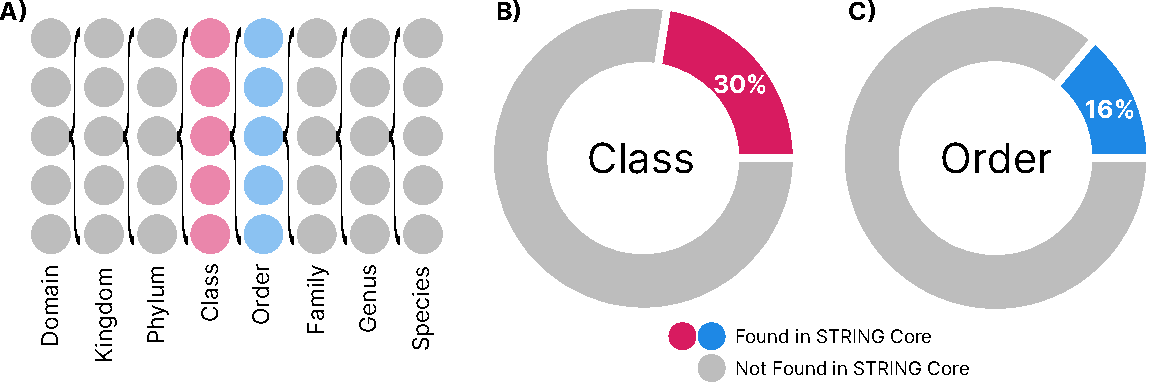
\includegraphics[scale=0.7]{figures/intrepppid/string_species_analysis-eps-converted-to.pdf}
    }
    \caption[The species gap as illustrated by the \textsc{string} \textsc{ppi} database.]{\textbf{\textsf{The species gap as illustrated by the STRING PPI database.}} \textbf{(A)} the hierarchy of biological taxa [9]. \textbf{(B, C)} Doughnut charts indicating the proportion of all taxa represented in \textsc{string} Core at the class rank \textbf{(B)} and order rank \textbf{(C)}.}\label{fig:intrepppid_species_gap}
\end{figure}

Regrettably, a major barrier to bridging the species gap is that there are often too few interaction data to train \textsc{ppi} inference models for lesser-studied organisms. In order for computational models to address the species gap, they must make accurate \textsc{ppi} inferences on less-studied organisms, while using existing \textsc{ppi} data from well-studied organisms during training. Such ‘cross-species’ inference can be used to infer the intraspecies \textsc{ppi} network of the less-studied organism, all while only using the model organism as training data, addressing the species gap. Cross-species inference requires that methods perform accurate out-of-distribution (\textsc{ood}) inference. Historically, \textsc{ppi} inference methods have failed to make accurate predictions on interactions between \textsc{ood} proteins [11–13].

In 2012, a letter published by Park and Marcotte outlined the severity of pervasive data leakage that was obscuring the inability of methods of the time to generalize to interactions between \textsc{ood} proteins [11]. The cause of the data leakage Park and Marcotte observed was the common ‘random splitting’ approach to preparing cross-validation folds. Random splitting of interactions (between pairs of proteins) into folds allows for the same proteins appearing in both the training and testing sets, resulting in data leakage. Park and Marcotte found that when methods of the time were trained and tested on ‘strict’ datasets where proteins present in the training set never appear in any of the other folds, the accuracy of most methods dropped to random levels. This precipitous drop in performance indicates that all the models tested had problems dealing with \textsc{ood} proteins.

While Park and Marcotte found that \textsc{ood} performance was poor across the landscape of methods available in 2012, studies by Dunham and Ganapathiraju in 2021 and Bernett \textit{et al.} in 2023 corroborate the 12-year-old findings [12, 13]. In both studies, contemporary sequence-based \textsc{ppi} inference methods were tested on datasets that satisfy Park and Marcotte’s strictest validation schemes. Predictive power dramatically degraded in all cases, just as Park and Marcotte observed in 2012. While models for \textsc{ppi} inference have changed drastically since 2012 with the notable introduction of deep learning methods, reported performance of methods continue to be inf lated as a result of the random splitting of interactions (as opposed to stricter splitting based on proteins).

Furthermore, work by Hamp and Rost as well as Bernett \textit{et al.} underscore an additional source of data leakage: distinct proteins with sequences which are nearly identical [13, 14]. Amino acid sequences can be overwhelmingly redundant between distinct proteins. An important consequence of this is that two proteins with all but identical sequences may appear in both sets, thereby leaking data in the same way randomly-splitting \textsc{ppi} pairs does. The challenges presented by sequence similarity can be overcome by ensuring that proteins in the training set do not have a sequence identity above some threshold with proteins in the testing set.

One of the earliest approaches for sequence-based \textsc{ppi} inference is Marcotte \textit{et al.}'s `Rosetta Stone' method [15]. The authors outline a theory whereby interacting proteins of one species sometimes appear as fused homologous proteins in other species. Using this technique, Marcotte \textit{et al.} inferred interactions between proteins from \textit{Escherichia coli} using information of proteins of other genomes that had similar sequences to the putative pair. The concept of `interologue' was soon after introduced to describe proteins whose interactions are conserved among their respective orthologues [16]. Interologues allow us to extend knowledge of interactions of one species to other species by identifying both sequences and interactions that are conserved between them [17, 18]. These homology-based methods, while effective at identifying conserved interactions, have limitations related to unknown interactions, as acknowledged in the work that first introduced the term interologue: `Although potentially powerful, applying the interologue concept alone in estimating the significance of potential interactions precludes the finding of novel connections previously unidentified in other model organisms' [16].

Some of the first machine-learning methods for predicting \textsc{ppi}s were kernel-based methods operating on sequence features. The support vector machine (\textsc{svm}) is an algorithm for finding the maximum-margin hyperplane for a classification or regression problem, relying on kernel transformations of the input data to solve nonlinear problems [19]. Effectively applying \textsc{svm}s to the problem of \textsc{ppi} classification depends greatly on the design of the kernels used to represent protein pairs. These kernels, designed by expert knowledge, may compare individual proteins to each other (`genomic kernels') or pairs of proteins to other pairs (`pairwise kernels'). Furthermore, these kernels may compare a variety of features of the gene products being studied, including motifs, gene ontology (\textsc{go}) annotations, sequence similarity, or some combination thereof [20].

As advances in hardware and algorithms made research into deep learning more feasible, they’ve proven to be effective in a number of problem domains, not least of which being \textsc{ppi} prediction. Richoux \textit{et al.} demonstrated that twin neural-networks are far more efficient at \textsc{ppi} inference than other network architectures [21]. Twin neural networks are models that consider pairs of inputs using the same trainable parameters rather than specifying parameters for each input and are commonly used to make comparisons between two inputs [22, 23]. Twin networks can reduce the risk of overfitting and aiding few-shot performance [24]. Many twin \textsc{ppi} prediction methods rely on convolutional neural networks (\textsc{cnn}s) or recurrent neural networks (\textsc{rnn}s) to encode feature sequences. The \textsc{pipr} method by Chen \textit{et al.}, however, eschews these architectures for a hybrid: the recurrent \textsc{cnn} (\textsc{rcnn}) [25]. The \textsc{rcnn} comprises of an initial \textsc{cnn} layer whose output is fed into a bidirectional gated recurrent unit (\textsc{gru}) \textsc{rnn} [26].

We’ve previously described \textsc{rapppid}, a method for \textsc{ppi} prediction that outperforms leading methods on strict validation sets that conform to the guidelines set out by Park and Marcotte [11, 27]. \textsc{rapppid} is a twin network that learns latent representations of sequences and inputs them into a classifier network to infer whether two proteins interact. \textsc{rapppid} achieves its high performance largely due to its adoption of averaged weight-decayed \textsc{lstm} (\textsc{awd-lstm}) and the Unigram tokenization algorithm [28, 29]. The former is a combination of regularization techniques that are effective for long short-term memory (\textsc{lstm}) \textsc{rnn}s. The input is tokenized using subword regularization, which regularizes the network by sampling from a distribution of different segmentations of the input [30].

In spite of the aforementioned progress in the field, most computational models are not designed to address the species gap and exhibit reduced performance when tested on the cross-species task. This makes them unsuitable to address the species gap problem and as such, the knowledge of the protein interactions that govern fundamental biological processes of ill-studied non-model organisms remains beyond our grasp. To address this issue, we introduce an extension of \textsc{rapppid} named \textsc{intrepppid} (Incorporating Triplet Error for Predicting \textsc{ppi}s using Deep Learning). \textsc{intrepppid} is specifically designed to improve cross-species \textsc{ppi} prediction performance with the aim of reducing the species gap. In this study, ‘cross-species’ \textsc{ppi} prediction refers to predicting the intraspecies interactions of proteins of one species using a computational model that is trained on intraspecies interactions of a different species. This term does not refer to predicting the interaction between one protein from one species and another protein from a different species.

We designed \textsc{intrepppid} to learn latent representations of amino acid sequences that are useful for predicting \textsc{ppi}s as well as identifying orthologues. Alongside \textsc{rapppid}’s original twin network for inference, \textsc{intrepppid} adds a triplet network that minimizes the Euclidean distance between latent representations of orthologous sequences while maximizing it for nonorthologous sequences. Parameters are shared between both the twin and triplet networks, resulting in five networks with a single set of shared parameters, which we call a ‘quintuplet’ network. \textsc{intrepppid}’s architecture learns a latent space that encodes both \textsc{ppi} and orthology information. This allows us to enforce an inductive bias loosely based on the concept of interologues.

The contributions of this study are as follows. First, we introduce \textsc{intrepppid}, a deep learning method based on a novel quintuplet architecture and a carefully designed loss function that makes out-of-distribution predictions of \textsc{ppi}s to address the species gap. Our analysis shows that \textsc{intrepppid} outperforms all leading methods tested on both intraspecies and cross-species \textsc{ppi} predictions. Second, we demonstrate that \textsc{intrepppid} effectively learns the orthology of proteins and its performance improvement is due to learning biologically relevant information. This suggests the use of orthology information as a powerful approach for making out-of-distribution predictions in this domain. Third, we have released to the community \textsc{ppi}.bio, an open-source interface for \textsc{intrepppid} and \textsc{rapppid} hosted on the internet. This allows researchers to infer \textsc{ppi}s without installing any specialized software or using the command line. Finally, we have released \textsc{ppi} Origami, a computer programme for creating reproducible strict \textsc{ppi} databases in an automated fashion. By automating the dataset generation process, we hope to reduce common sources of data leakage in datasets used for \textsc{ppi} inference.

\section*{Materials and methods}
\label{sec:intrepppid_methods}
\addcontentsline{toc}{section}{Materials and methods}

\subsection*{The INTREPPPID architecture}
\addcontentsline{toc}{subsection}{The \textsc{intrepppid} architecture}

\textsc{intrepppid} integrates \textsc{rapppid}'s twin network for the \textsc{ppi} Classification task with a triplet neural network used for a novel Orthologous Locality task. Learning the two networks jointly results in five encoder layers with shared parameters in what we’ve come to call a quintuplet network architecture.

\textsc{intrepppid} uses the same \textsc{awd-lstm} encoder as the one used in \textsc{rapppid} to learn vector representations of protein sequences. This encoder is a regularized \textsc{rnn} that has been shown to improve performance on tasks that require inferring interactions between proteins absent from the training set [27]. Before encoding, sequences are first tokenized using the Unigram algorithm as implemented by the SentencePiece library [29, 30]. \textsc{intrepppid} uses the vector representations generated by the encoder for two downstream tasks: the `orthologous locality' task and the `\textsc{ppi} classification' task. The encoder as well as the two tasks are trained in an end-to-end fashion.

\textsc{intrepppid}'s quintuplet architecture means that training the network relies on additional orthology data. At inference time, however, only the protein classification twin network is used, so no information other than the amino acid sequences of the proteins in question are required as input.

\subsection*{The protein–protein interaction classification task}
\addcontentsline{toc}{subsection}{The protein–protein interaction classification task}
\textsc{intrepppid} infers \textsc{ppi}s by learning latent representations of the candidate protein sequences which can be classified by a fully connected neural network outputting the interaction probability. The two amino acid sequences ($s_β$ and $s_γ$ ) are first tokenized into vectors $x_β$ and $x_γ$ using the Unigram algorithm. The Unigram algorithm segments the amino acid of the protein sequence into groups using a vocabulary of 250 tokens. The Unigram algorithm also employs subword regularization. Unigram draws tokens for a given sequence from a probabilistic distribution of all possible combination of tokens in the vocabulary, meaning that the same sequence can be tokenized differently between successive calls to the tokenizer.

Once the tokenized vectors $x_β$ and $x_γ$ are obtained, they are inputted into an encoder ($e(\cdot)$) that outputs a latent vector for each protein ($z_β$ and $z_γ$ , respectively):

\begin{align*}
  z_\beta = e(x_\beta)\\
  z_\gamma = e(x_\gamma).
\end{align*}

Finally, the latent vectors $z_\beta$ and $z_\gamma$ are averaged and inputted into a classifier network $g(\cdot)$ that outputs an interaction probability $\hat{y}$:

$$
y = g\left(\left(z_\beta + z_\gamma \right) /2\right) .
$$

The classifier $g(\cdot)$ is a two-layer, fully connected neural network whose hidden layer is activated by the Mish function [31]. The fully connected neural network outputs a single real number which, once activated by the sigmoid function, represents the probability that the proteins represented by the amino acid sequences $s_\beta$ and $s_\gamma$ interact. This interaction probability as well as the true label are inputted into the binary cross-entropy loss to obtain a loss for the \textsc{ppi} classification network:

$$
\mathcal{l}_\textrm{class} = (\hat{y}, y) = −y \cdot \log(\hat{y}) + (1 − y) \cdot \log (1 − \hat{y}) ,
$$

where $y$ is a binary label representing whether the two proteins truly interact ($y = 1$) or not ($y = 0$).

\subsection*{The orthologous locality task}
\addcontentsline{toc}{subsection}{The orthologous locality task}
\textsc{intrepppid} introduces a novel task to help inform the \textsc{ppi} classification network. The orthologous locality task is to learn a latent space whereby the Euclidean distance between latent representations of proteins that are orthologous to one another are within some margin $m$. Conversely, nonorthologous proteins are to have a Euclidean distance greater than $m$.

To achieve this, we adopt a triplet network and a triplet margin loss $\mathcal{l}_\textrm{ortho}$ following the description of [32]:

$$
\mathcal{l}_\textrm{ortho}(z_a, z_p, z_n ) = \max (d (z_a, z_p) − d (z_a, z_n) + m , 0) ,
$$

where $z_a$ is the latent vector of some `anchor' protein for which there is a known orthologous protein with a latent vector $z_p$, $z_n$ is the latent vector of a randomly chosen protein that is not an orthologue of $z_a$, $m$ is a margin factor and $d$ is the Euclidean distance:

$$
d(u, v) = ||u − v||^2.
$$

For the experiments conducted herein, the margin $m$ was fixed at a value of 1.

The principle of the triplet network is to, at every training step, maximize the distance between two nonorthologous proteins (the `anchor' and `negative' proteins), as well as minimize the distance between two orthologous proteins (the `anchor' and `positive' proteins).

The anchor protein, with amino acid sequence $s_a$, can be any protein in the dataset for which orthology data are known. All orthology data for the experiments conducted herein are from the Orthologous Matrix (\textsc{oma}) database of orthologues [33]. In the event that orthologues are known for the protein that $s_\beta$ encodes, $s_\beta$ is chosen to be $s_a$.

The positive and negative proteins (with amino acid sequences $s_p$ and $s_n$, respectively) are chosen relative to $s_a$. $s_p$ is chosen to be the sequence of a randomly chosen protein that, according to the \textsc{oma} database, belongs to the set of sequences of proteins orthologous to the anchor protein. At every training step, $s_p$ is drawn randomly from this set of proteins orthologous to $s_a$, meaning that the positive protein for a given anchor protein may not be the same between training steps or epochs. The negative protein is sampled in a similar manner to the positive protein, but rather than being sampled from the set of proteins orthologous to $s_a$, is sampled from the set of proteins not orthologous to $s_a$. The amino acid sequence of the anchor, positive, and negative proteins ($s_a$, $s_p$, and $s_n$) are tokenized and encoded in the same manner as $s_\beta$ and $s_\gamma$ , resulting in their latent representations $z_a$, $z_p$, and $z_n$.

Optimizing the triplet margin loss in this manner maximizes the Euclidean distance between latent vectors of proteins that are not orthologues, while minimizing the distance between vectors of orthologues. Our adoption of the triplet margin loss follows evidence that such a loss is an effective way of creating feature descriptors that are `spread out' over the latent space, which in turn increases performance on downstream classification tasks [32, 34]. Furthermore, orthologues typically share the same protein functions and therefore offer a good interspecies basis for the downstream \textsc{ppi} classification task [35, 36].

\subsection*{INTREPPPID’s loss function}
\addcontentsline{toc}{subsection}{\textsc{intrepppid}’s loss function}

The final \textsc{intrepppid} loss function that is optimized at training time is the sum of $\mathcal{l}_\textrm{ortho}$ and $\mathcal{l}_\textrm{class}$,

$$
\hat{L}(\hat{y},y,z_a,z_p,z_n) = \mathcal{l}_\textrm{class}(\hat{y},y) + \mathcal{l}_\textrm{ortho}(z_a, z_p, z_n).
$$

In this way, \textsc{intrepppid} optimizes both the orthologous locality and \textsc{ppi} classification losses simultaneously, in an end-toend fashion, ensuring that latent vectors simultaneously encode orthology and \textsc{ppi} information.

\subsection*{Preparing strict protein–protein interaction datasets}
\addcontentsline{toc}{subsection}{Preparing strict protein–protein interaction datasets}

Experiments were run using datasets with strict data splitting folds, described as `\textsc{c3}' by Park and Marcotte [11]. Namely, we ensured that there was no overlap of proteins between any of the training, validation, or testing datasets. Additionally, we controlled for sequence similarity of proteins between the training, validation, and testing sets that is a known vector for information leakage [13, 14]. We specifically control to ensure that proteins with $>90\%$ sequence identity are not present between splits to ensure that proteins that differ only by name are not accidentally present in two different splits. Another reason for choosing a threshold of 90\% sequence identity is that it allows us to test the ability of \textsc{intrepppid} to learn motifs and domains relevant to interactions. Individuals who wish to create testing datasets that limit the exposure of similar motifs and domains can create those with more strict sequence identity requirement (\textit{e.g.} a 50\% threshold) using \textsc{ppi} Origami (see Generating Strict Protein–Protein Interaction Datasets with Protein–Protein Interaction Origami). Protein interaction data are obtained from the \textsc{string} database, version 12 [8]. Interactions with a confidence score $<90\%$ are filtered. \hyperref[sec:intrepppid_supp_methods]{Supplementary Methods} provide details of how we created such strict datasets, and Supplementary Table \hyperref[sec:intrepppid_supp_s1]{S1} outlines summary statistics for the datasets used in this study.

\subsection*{Generating strict protein–protein interaction datasets with protein–protein interaction origami}
\addcontentsline{toc}{subsection}{Generating strict protein–protein interaction datasets with protein–protein interaction origami}
We have written a command-line interface (\textsc{cli}) tool named `\textsc{ppi} Origami' with the aim of making the task of preparing strict \textsc{ppi} datasets in a replicable and automated fashion. \textsc{ppi} Origami has three primary functions: `downloading' primary databases, `processing' primary databases into strict datasets, and an `analysis' function.

\textsc{ppi} Origami allows for the downloading of primary databases as an integrated part of its pipeline. By directly handling downloading third-party databases, \textsc{ppi} Origami ensures that different users of the software are downloading the same files in the same way. \textsc{ppi} Origami also stores downloaded files in a distinct location from the processed files, isolating primary files from accidental changes.

\textsc{ppi} Origami’s main function is to process and transform primary databases into strict \textsc{ppi} datasets. It can create datasets that satisfy both criteria of strict \textsc{ppi} datasets, filtering low-confidence positive examples, and drawing negative examples as previously described.

\textsc{ppi} Origami allows for simple reporting of basic statistics of \textsc{ppi} datasets it generates. These reports allow for convenient verification of whether datasets meet both criteria of strict datasets, as well as other statistics of interest such as the ratio of interactions between dataset cross-validation subsets.

We hope that \textsc{ppi} Origami encourages other researchers to incorporate strict \textsc{ppi} datasets in the future development and analyses of supervised \textsc{ppi} inference methods.

\subsection*{Training procedure}
\addcontentsline{toc}{subsection}{Training procedure}
\textsc{intrepppid} was trained using the Ranger21 optimizer, which uses AdamW with a look-ahead mechanism [37, 38]. An `explore-and-exploit' learning rate scheduler was used, with a maximum learning rate of 0.01 [39]. \textsc{intrepppid} was trained for 100 epochs. The weights of the epoch with the lowest validation loss were used in the analyses herein (and for evaluation on the test set). Hyperparameters used to train \textsc{intrepppid} were informed by those selected during the development of \textsc{rapppid} and are listed in Supplementary Table \ref{tab:intrepppid_supp_hyperparameters}.

\section*{Results}
\addcontentsline{toc}{section}{Results}

\subsection*{INTREPPPID outperforms leading models for prediction of human protein–protein interaction}
\addcontentsline{toc}{subsection}{\textsc{intrepppid} outperforms leading models for prediction of human protein–protein interaction}

First, we set out to evaluate the performance of \textsc{intrepppid} (Fig. \ref{fig:intrepppid_architecture_intra}A) in an intraspecies \textsc{ppi} prediction task: trained and tested on \textit{Homo sapiens} interactions in the \textsc{string} database (see Materials and Methods). Table \ref{tab:intrepppid_perf} shows the performance of \textsc{intrepppid} against five leading \textsc{ppi} prediction methods. These methods include \textsc{rapppid}, our previous method upon which \textsc{intrepppid} expands, \textsc{d-script}, a method designed for the cross-species task, \textsc{pipr}, a twin network with an \textsc{rcnn} encoder, \textsc{sprint}, a sequence-similarity-based method, and the twin networks proposed by Richoux \textit{et al.} [21, 25, 27, 40, 41]. \textsc{intrepppid} performed slightly better than \textsc{rapppid} across all metrics and outperformed all other methods (Table \ref{tab:intrepppid_perf}, Fig. \ref{fig:intrepppid_architecture_intra}B, Supplementary Table \hyperref[sec:intrepppid_supp_s3]{S3}). Richoux \textit{et al.}, \textsc{d-script}, and \textsc{sprint} perform similarly on average, with \textsc{d-script} exhibiting a particularly high degree of variability across the different datasets tested. We observed severe over-fitting while training and testing \textsc{pipr} on all datasets. Precision–recall and receiver-operator Curves are reported in Supplementary Figs \ref{fig:intreppid_supp_pr} and \ref{fig:intreppid_supp_roc}, respectively.

\begin{figure}[h!]
	\centerline{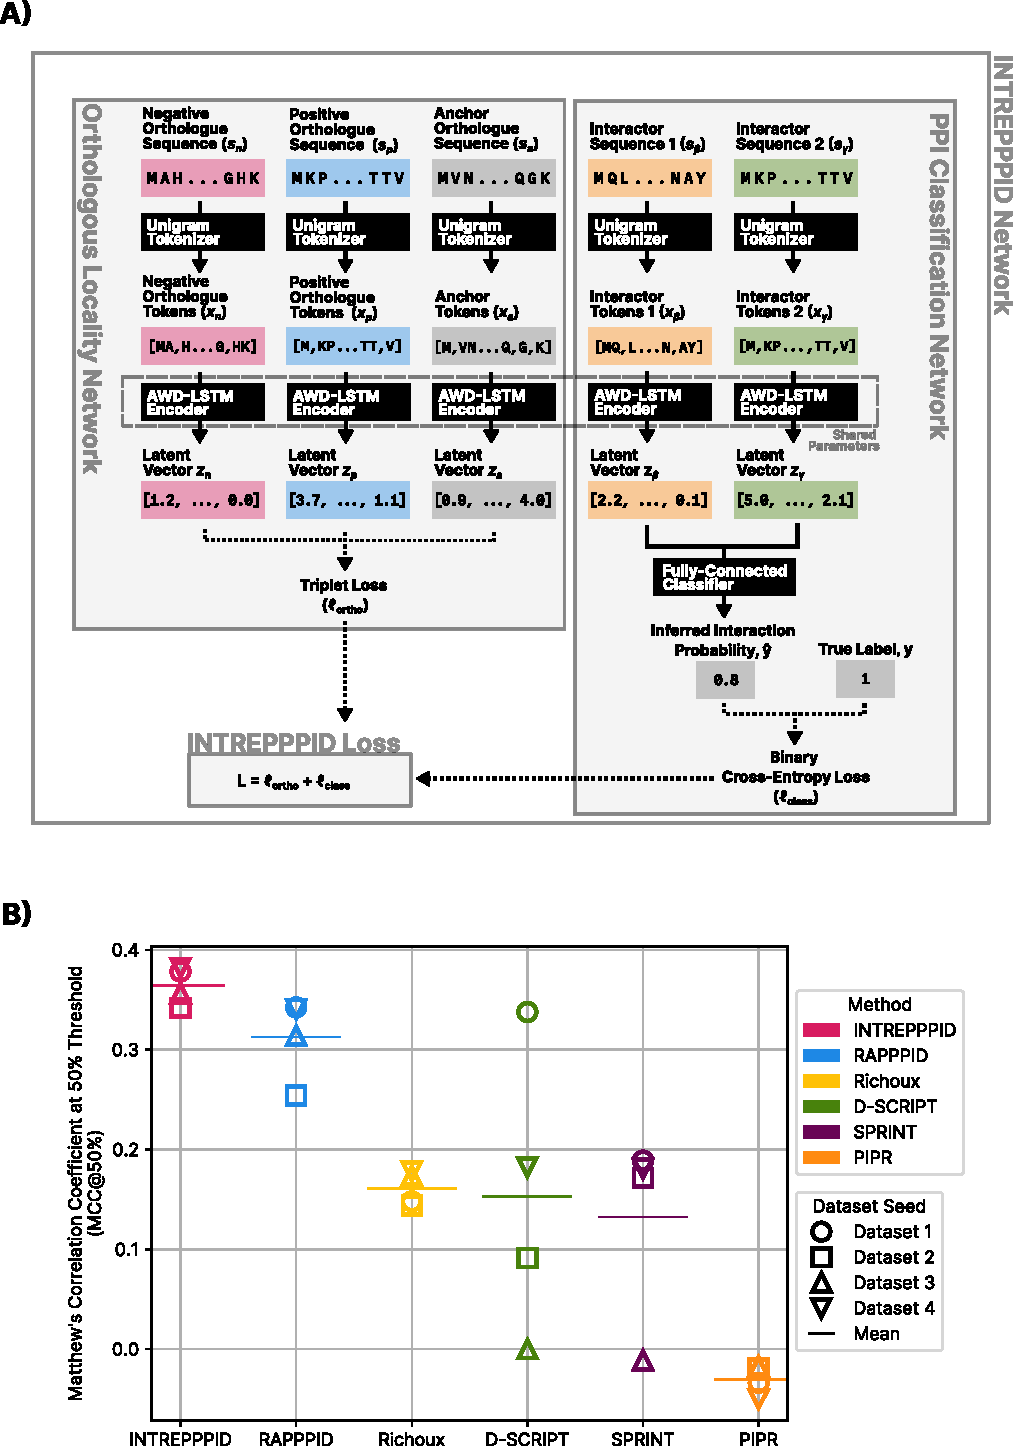
\includegraphics[scale=0.7]{figures/intrepppid/architecture_intra.pdf}
    }
    \caption[INTREPPPID’s architecture and performance.]{\textbf{\textsf{INTREPPPID’s architecture and performance.}} \textbf{(A)} A schematic overview of \textsc{intrepppid}’s quintuplet architecture. The leftmost panel depict s the triplet network responsible for the orthologous locality task, while the rightmost panel depicts the triplet network responsible for the \textsc{ppi} classification task. During training, \textsc{intrepppid} learns both tasks jointly through an overall loss function, which is the sum of the losses of the two tasks. \textbf{(B)} Test (\textsc{c3}) Matthew’s correlation coefficient (\textsc{mcc}) of leading \textsc{ppi} inference methods trained and tested on \textit{H.~sapiens} datasets.} \label{fig:intrepppid_architecture_intra}
\end{figure}

Unlike our benchmarks, it is estimated that there are far more pairs of proteins that do not interact than those that do [6, 42]. Accordingly, we tested \textsc{intrepppid}’s performance at increasing negative-to-positive interaction ratios and found that no appreciable change in performance was found (Supplementary Table \ref{tab:intrepppid_supp_neg_ratio}).

\begin{table}[!t]
    \label{tab:intrepppid_perf}
	\caption[Average performance of five leading \textsc{ppi} inference methods trained and tested on four \textit{H.~sapiens} \textsc{ppi} datasets.]{\textsf{\textbf{Average performance of five leading PPI inference methods trained and tested on four \textit{H.~sapiens} PPI datasets.}} The performance metrics are calculated on strict \textsc{c3} test sets (see \hyperref[sec:intrepppid_methods]{Materials and Methods}). The upward arrow (▲) indicates higher values are better for a metric, whereas a downward arrow (▼) indicates lower value are better. Boldface indicates the best value. The following abbreviations are used: \textsc{auroc}: area under the receiver operating characteristic; \textsc{ap}: average precision; \textsc{mcc}: Matthew’s correlation coefficient, \textsc{sd}: standard deviation. \label{tab:intrepppid_perf}} {\begin{tabular}{@{}lllllll@{}}\toprule 
			Method & INTREPPID & \textsc{rapppid} & \textsc{d-script} & Richoux \textit{et al.} & \textsc{sprint} & \textsc{pipr} \\\midrule
			▲ \textsc{auroc} & \textbf{0.752} & 0.732 & 0.634 & 0.606& 0.597& 0.482\\
            Mean (±\textsc{sd}) & (± 0.017) & (± 0.024) & (± 0.125) & (± 0.009)& (± 0.061)& (± 0.006)\\
            ▲ \textsc{ap} & \textbf{0.730} & 0.717 & 0.627 & 0.614& 0.641& 0.484\\
            Mean (±\textsc{sd}) & (± 0.022) & (± 0.015) & (± 0.086) & (± 0.015)& (± 0.064)& (± 0.003)\\
            ▲ \textsc{mcc}{@}50\% & \textbf{0.365} & 0.313 & 0.153 & 0.161& 0.133& -0.030\\
            Mean (±\textsc{sd}) & (± 0.067) & (± 0.041) & (± 0.144) & (± 0.017)& (± 0.096)& (± 0.015)\\
            ▲ $F_1${@}50\% & \textbf{0.697} & 0.630 & 0.506 & 0.370& 0.566& 0.318\\
            Mean (±\textsc{sd}) & (± 0.019) & (± 0.025) & (± 0.282) & (± 0.030)& (± 0.048)& (± 0.010)\\
            ▼ Brier Score & \textbf{0.200} & 0.215 & 0.402 & 0.274& 0.493& 0.487\\
            Mean (±\textsc{sd}) & (± 0.004) & (± 0.006) & (± 0.116) & (± 0.011)& (± 0.003)& (± 0.005)\\
			\midrule
	\end{tabular}}{}

\end{table}

\subsection*{INTREPPPID maintains high cross-species performance on multiple organisms}
\addcontentsline{toc}{subsection}{\textsc{intrepppid} maintains high cross-species performance on multiple organisms}

\textsc{intrepppid} was designed to improve on \textsc{rapppid}'s ability to make predictions across species. We therefore sought to compare \textsc{intrepppid}'s cross-species performance with that of \textsc{rapppid}'s as well as other leading \textsc{ppi} prediction methods.

When trained on \textit{H.~sapiens} and tested on various species (\textsc{c3}), ranging from \textit{Mus musculus} (house mouse) to \textit{Arabidopsis thaliana} (thale cress), \textsc{intrepppid} predominantly outperformed other methods (Fig. \ref{fig:intrepppid_cross_species}A, Supplementary Table \hyperref[sec:intrepppid_supp_s5]{S5}), with only \textsc{rapppid} rarely surpassing its performance in some metrics. Figure \ref{fig:intrepppid_cross_species}A shows the mean \textsc{auroc} (across three datasets) of different methods, with \textsc{intrepppid} significantly outperforming all other methods (one-sided Wilcoxon signed rank test versus \textsc{rapppid} = 0.03). On the cross-species task, the performance of \textsc{pipr} and \textsc{sprint} were close to a random classifier. Both \textsc{d-script} and the Richoux \textit{et al.} method performed similarly to one another, but consistently scored below \textsc{rapppid} and \textsc{intrepppid}.

In many applications, one is particularly interested in the precision of a model among the highest-ranking predicted edges (\textit{e.g.} to validate them experimentally). To evaluate \textsc{intrepppid}’s suitability for such tasks, we measured the precision of predictions whose scores are above various percentiles (Fig. \ref{fig:intrepppid_cross_species}B). Considering the average across all species tested, \textsc{intrepppid} achieved a precision $>90\%$ among predictions above the 85th percentile, and even when we considered the 75th percentile, its mean precision remained $>85\%$. These observations confirm that \textsc{intrepppid} is suitable for applications where very high precision is paramount.
\begin{figure}[h!]
	\centerline{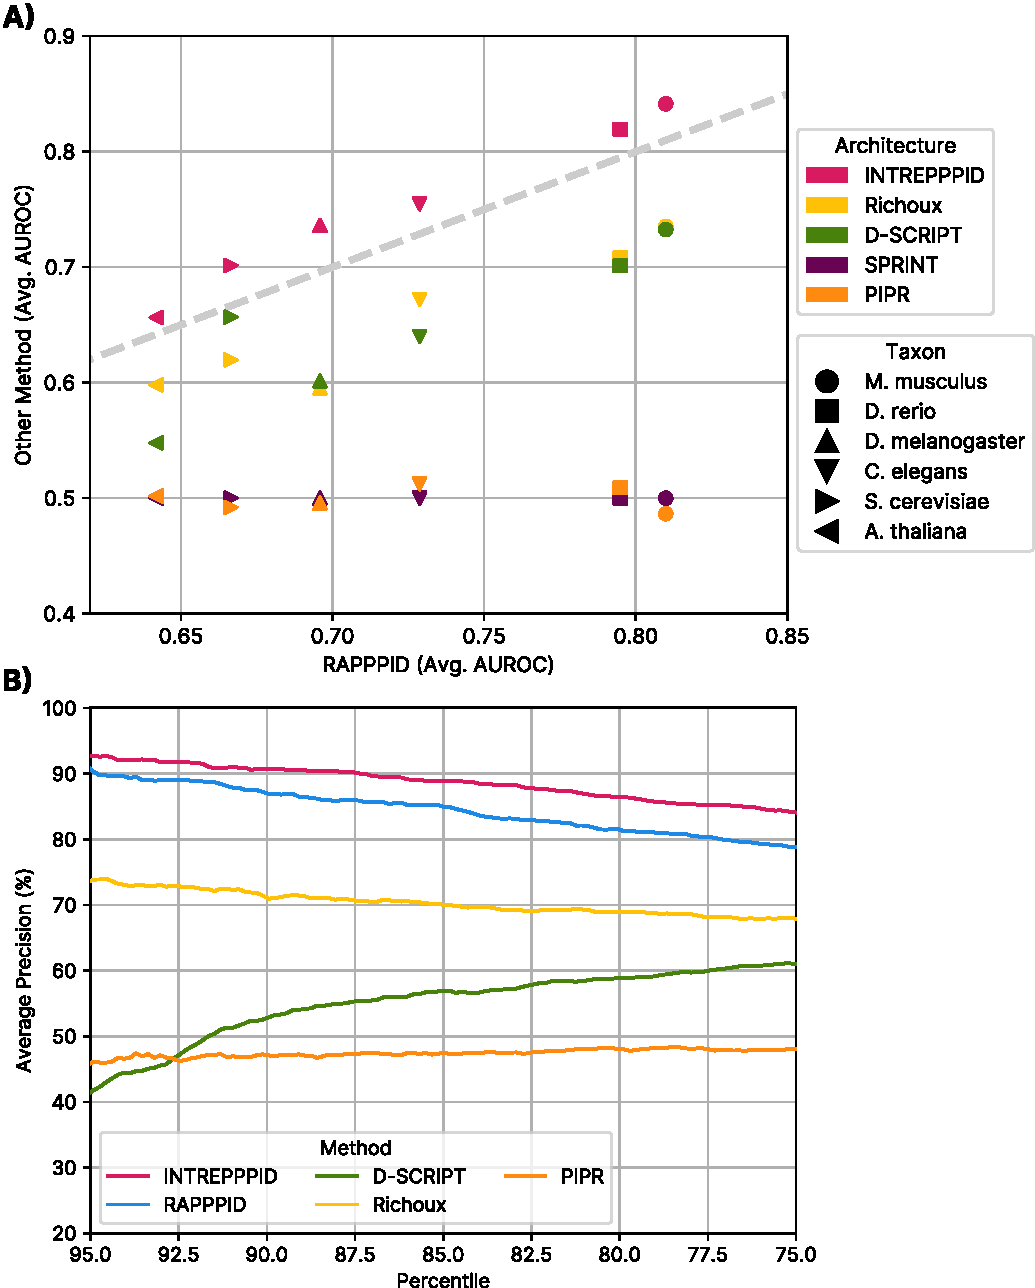
\includegraphics[scale=0.7]{figures/intrepppid/cross_species2.pdf}
    }
    \caption[Cross-species performance]{ \textbf{(A)} Average cross-species AUROC of leading \textsc{ppi} inference methods. The y-axis shows the \textsc{auroc} of each method (shown as different colours) against the \textsc{auroc} of \textsc{rapppid} (x-axis). Each model was trained on H.~sapiens and tested on various species (indicated by the different markers). Markers above the dashed grey line indicate instances where a method outperformed \textsc{rapppid}, while markers below the line indicate under-performance. \textbf{(B)} The precision of inferred interactions among the $k^\textrm{th}$ percentile of the scores inferred by the method indicated by the line colour. The x-axis shows $k$ and the y-axis shows precision along the y-axis. Interactions were inferred for datasets from seven different species. The mean across these datasets is reported by the solid line.}\label{fig:intrepppid_cross_species}
\end{figure}

We sought to further confirm \textsc{intrepppid}’s ability to generalize by measuring the number of interactions in additional \textsc{ppi} databases that \textsc{intrepppid} was capable of recovering. When considering interactions with confidence scores of 95\% or higher, \textsc{intrepppid} was capable of correctly identifying 72\% of interaction in the \textsc{hippie} database and 69\% of interaction in the IntAct database. These results are only slightly lower than the 74\% true-positive rate \textsc{intrepppid} achieves on our benchmark dataset.

\subsection*{INTREPPPID learns protein representations that exhibit strong orthologous locality}
\addcontentsline{toc}{subsection}{\textsc{intrepppid} learns protein representations that exhibit strong orthologous locality}
Through its orthologous locality task, \textsc{intrepppid} learns latent representations of orthologues that are near to one another in the Euclidean space, while ensuring latent representations of nonorthologous sequences remain distant. To qualitatively assess the locality of orthologues in latent space, we calculated the embeddings of the sequences of 1000 randomly sampled proteins present in the \textsc{oma} database of orthologues and projected them onto a \textsc{2d} space using \textsc{umap} and \textsc{pca} (Supplementary Fig. \ref{fig:intreppid_supp_scramble}) [43]. The projections show that embeddings of orthologues cluster tightly in \textsc{intrepppid}’s latent space, while embeddings from \textsc{rapppid} (which has a similar architecture, but without the triplet network) do not.

A more quantitative analysis of embedding distances further confirmed that \textsc{intrepppid}'s latent space exhibits strong orthologous locality. Namely, the Euclidean distance between latent representations of orthologues was on average 0.822, while the distance between the representations of nonorthologous proteins is on average 5.31 (Supplementary Fig. \ref{fig:intreppid_supp_scramble}C). Nearly 80\% of \textsc{intrepppid}'s latent representations of orthologues fell under the triplet loss margin of 1, while virtually all nonorthologues had a distance greater than the margin between them.

Together, these analyses confirm that \textsc{intrepppid} successfully accomplishes the orthologous locality task.

\subsection*{INTREPPPID's performance gain is due to the biologically relevant information encoded by orthology}
\addcontentsline{toc}{subsection}{\textsc{intrepppid}'s performance gain is due to the biologically relevant information encoded by orthology}

To further assess the role of orthology information on the performance of \textsc{intrepppid}, we conducted an experiment in which we trained \textsc{intrepppid} on two separate datasets: one constructed using orthologue data from the \textsc{oma} database (called `not scrambled') and one where `random' pairs of proteins from the \textsc{oma} database were labelled orthologues (`scrambled'). After training and testing on both variants of the \textit{H.~sapiens} dataset, we found that \textsc{intrepppid}’s performance dropped to near random in the `scrambled' case (Supplementary Table \ref{tab:intrepppid_supp_scramble}, \textsc{auroc} = 0.524). Moreover, on this dataset, neither the classification loss nor the triplet loss significantly changed over 30~000 training steps (Supplementary Fig. \ref{fig:intreppid_supp_scramble}D).

\textsc{intrepppid}'s low testing performance on `scrambled' data suggests that the mere exposure of sequences from various species is not sufficient to increase \textsc{ppi} classification performance. The impact of the `scramble' dataset on both the classification and triplet losses suggests that the orthologous locality task is complimentary to the \textsc{ppi} classification task. Ablating the biological meaning of the orthology data conversely results in the orthologous locality task negatively impacting \textsc{ppi} classification performance. These results show that the encoding of orthology information increases \textsc{intrepppid}'s performance due to its biological relevance.

Having established that the central contribution of incorporating orthologues in the \textsc{intrepppid} model is the biological information they encode, we continued to test the extent to which they are relevant to \textsc{intrepppid}'s performance. To do so, we constructed \textsc{intrepppid} datasets of \textit{H.~sapiens} protein interactions much as we have for previous cross-species analyses herein. For this analysis, however, orthology data related to proteins belonging to any of the testing species (\textit{H.~sapiens}, \textit{M.~musculus}, \textit{Danio rerio}, \textit{Drosophila melanogaster}, \textit{Caenorhabditis elegans}, \textit{Saccharomyces cerevisiae}, \textit{A.~thaliana}) were omitted. Relative to \textsc{intrepppid} trained on dataset that included all available orthology data, the altered dataset resulted in worse testing performance metrics across every species tested (Supplementary Table \ref{tab:intrepppid_supp_no_ortho}). The decrease in performance was least severe when testing on \textit{H.~sapiens} (\textit{i.e.} intraspecies inference), having measured a $−9.00\%$ change in \textsc{mcc} and $−1.36\%$ change in \textsc{ap} scores. Conversely, the performance drop was much greater on testing sets of species different from the training species (\textit{i.e.} cross-species inference), with observed changes as low as $−38.85\%$ for \textsc{mcc} and $-17.58\%$ for \textsc{ap} scores in some instances. This further confirms that orthology information is used by the model to make predictions.

\subsection*{INTREPPPID learns interactions of evolutionarily conserved functions that RAPPPID does not}
\addcontentsline{toc}{subsection}{\textsc{intrepppid} learns interactions of evolutionarily conserved functions that \textsc{rapppid} does not}

To better understand the biological characteristics of the interactions that account for \textsc{intrepppid}’s performance gains and the role that its orthology loss plays, we analysed the pairs of interacting proteins from our testing datasets in which \textsc{intrepppid} predicted a higher probability of interaction than \textsc{rapppid} by the widest margin. We found that, on average, \textsc{intrepppid} assigns higher scores to interacting pairs in 73\% ($\pm11\%$) of all cases. Of those inferred interactions, the top interactions were disproportionately between proteins that are evolutionarily conserved between species.

Our analysis began with pairs of proteins in the testing dataset that interact and were correctly identified by \textsc{intrepppid} (\textit{i.e.} a score $\geq0.5$), and incorrectly identified by \textsc{rapppid} (\textit{i.e.} a score $<0.5$). To examine cases in which most typified \textsc{intrepppid} are performing well while \textsc{rapppid} are falling short, we further filtered the aforementioned interactions such that only protein pairs with the largest differences between the \textsc{intrepppid} and \textsc{rapppid} scores remained (\textit{i.e.} in the 90th percentile or higher). These scored protein pairs will be referred to as `top \textsc{intrepppid} unique positive hits' hereafter.

A statistical analysis of over-representation of Gene Ontology (\textsc{go}) Molecular Function annotations was performed on the top \textsc{intrepppid}-unique positive hits using the \textsc{panther} Classification System [44–46]. This analysis provided us with an understanding of which \textsc{go} Molecular Function annotations were over-represented among proteins that comprised the top \textsc{intrepppid}-unique positive hits, relative to those in the testing set as a whole.

We found that, across the species tested, the \textsc{go} Molecular Function annotations that were overexpressed were primarily regarding ubiquinone activity, ribosome structure, and \textsc{rna} binding (Supplementary Table \hyperref[sec:intrepppid_supp_s8]{S8}). These functions all belong to pathways that are consistently found to be highly conserved across a broad spectrum of species [18, 47, 48].

An example of one of these interactions is one between the large ribosomal subunit proteins uL24A and uL10 found in \textit{S. cerevisiae} encoded by the genes \textit{RPL26A} and \textit{RPP0}, respectively. \textsc{intrepppid} correctly predicts that these two proteins interact with a probability of 94.6\% while \textsc{rapppid} assigns a probability of 4.52\%, both models having been trained exclusively on interactions between human proteins. The two proteins in question are highly conserved, with 131 and 798 orthologues recorded in the \textsc{oma} database for each protein, respectively. In both cases, a human orthologue is identified by \textsc{oma} (\textit{RPL26L1} and \textit{RPLP0} genes, respectively).

These observations suggests that \textsc{intrepppid} correctly identifies interactions that have functions crucial to pathways such as protein degradation and protein translation that are highly conserved between species, that \textsc{rapppid} does not. In addition, these observations provide further support that the discrepancy between \textsc{intrepppid} and \textsc{rapppid}’s performance among interactions composed of highly conserved proteins is driven by the similarity of embeddings among orthologous proteins (\textit{i.e.} the orthologous locality property), which is the primary distinction between \textsc{intrepppid} and \textsc{rapppid}.

\subsection*{A web server and interface for RAPPPID \& INTREPPPID}
\addcontentsline{toc}{subsection}{A web server and interface for \textsc{rapppid} \& \textsc{intrepppid}}
While we have made best efforts to make \textsc{rapppid} and \textsc{intrepppid} as simple as possible to run on a local computer with minimal computational requirements, it currently requires knowledge of the \textsc{cli} and the Python computer language. These prerequisites, while accessible to researchers with relevant experience, can be too great a hurdle for others.

To address this, we have created a website which acts as a graphical interface for a server that is capable of performing proteome-scale inference in under 15 min (\href{https://ppi.bio}{https://ppi.bio}). The source code that runs \textsc{ppi}.bio is available publicly on GitHub and can be found by visiting the internet address: \href{https:// github.com/Emad-COMBINE-lab/ppi.bio}{https:// github.com/Emad-COMBINE-lab/ppi.bio}. Many online academic servers are no longer available online and do not provide their source openly, resulting in the total loss of these servers (see Supplementary Table \ref{tab:intrepppid_supp_links} for a review of 22 such resources, 50\% of which are no longer alive). We hope to enable others to run their own server in the event that \href{https://ppi.bio}{https://ppi.bio} goes off line by releasing its code and documentation.

\begin{figure}[h!]
	\centerline{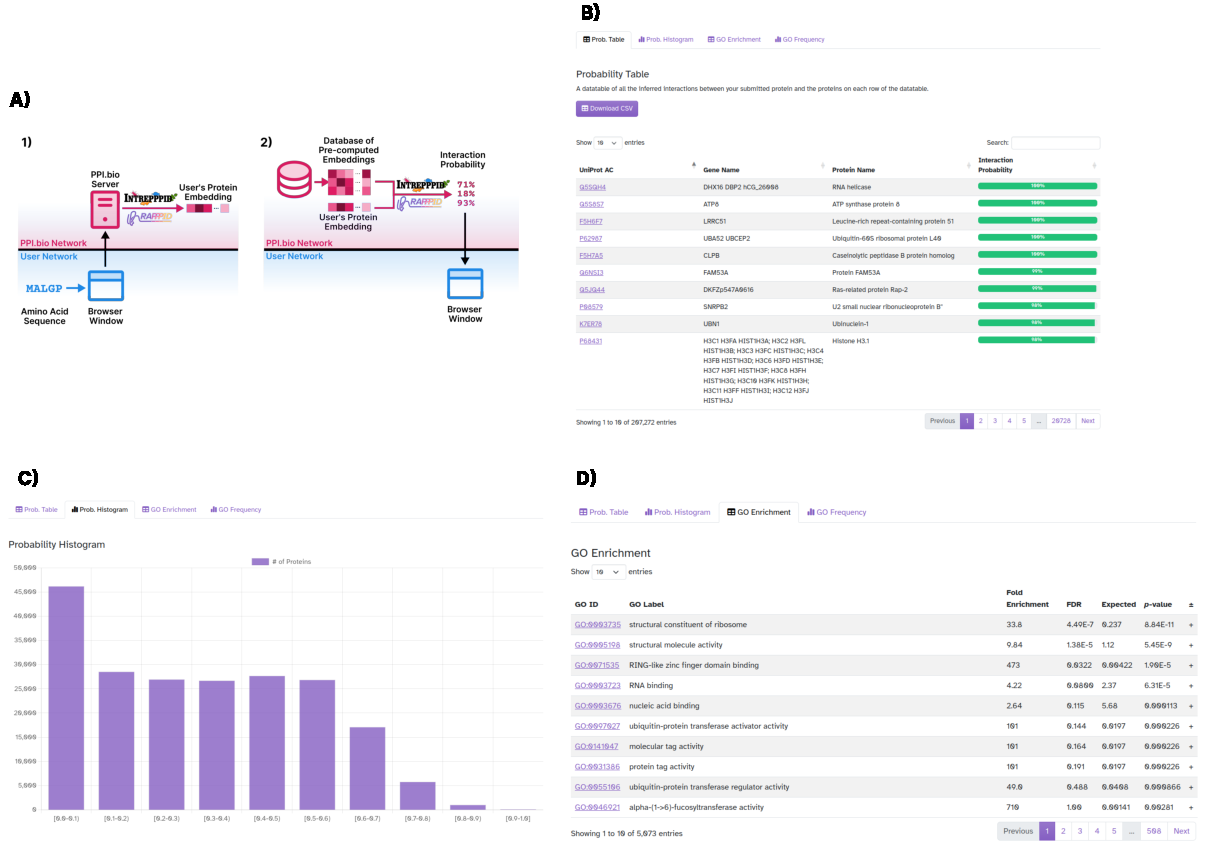
\includegraphics[scale=0.7]{figures/intrepppid/ppibio_screens.pdf}
    }
    \caption[The webserver of \textsc{ppi}.Bio supporting \textsc{rapppid} and \textsc{intrepppid} at whole proteome scale.]{\textbf{\textsf{The webserver of PPI.Bio supporting RAPPPID and INTREPPPID at whole proteome scale.}} \textbf{(A)} Overview of the operation of the \textsc{ppi}.Bio \textsc{ppi} inference server. In the first stage (leftmost panel), amino acid sequences are encoded into protein embeddings using either \textsc{rapppid} or \textsc{intrepppid}, depending on the user’s preference. In the second stage (rightmost panel), precomputed protein embeddings of a specified species proteome are loaded from a database. The classification head of either \textsc{rapppid} or \textsc{intrepppid} is then used to compute the probability of interaction of the user-specified protein and the precomputed embeddings. Screenshot of the \textbf{(B)} data table of interaction probabilities, \textbf{(C)} probability histograms, and \textbf{(D)} \textsc{go} enrichment analysis powered by \textsc{pantherdb}, as seen on \textsc{ppi}.Bio after inferring proteome-wide interactions.}\label{fig:intrepppid_ppi_bio}
\end{figure}

The process for making proteome-wide inferences on user-submitted amino acid sequence is as follows. Users input amino acid sequences that are then submitted to the \textsc{ppi}.bio server (Fig. \ref{fig:intrepppid_ppi_bio}). The \textsc{ppi}.bio server in turn encodes the sequence using the user’s choice of either \textsc{rapppid} or \textsc{intrepppid}’s encoder to obtain a protein embedding. The embedding is then paired with precomputed embeddings of all proteins belonging to the proteome of the user’s choosing (currently, proteins for six organisms have been computed). The probability of these pairs of proteins interacting are then inferred using \textsc{rapppid} or \textsc{intrepppid}’s classification head (based on the user’s choice), and returned to the user’s browser window.

\textsc{ppi}.bio also enables users to conduct \textsc{go} enrichment analysis on the set of proteins that have an interaction probability greater than some user-specified threshold. \textsc{ppi}.bio uses the \textsc{panther} online \textsc{api} [44] to calculate \textsc{go} enrichment statistics. This functionality allows users to find instances of \textsc{go} annotations being statistically over-represented among proteins that were inferred to interact with the protein supplied by the user.

\section*{Discussion}
\addcontentsline{toc}{section}{Discussion}
This study introduces three tools for researchers in their pursuit of better understanding \textsc{ppi}s: a cross-species method for \textsc{ppi} inference (\textsc{intrepppid}), a software package for creating strict \textsc{ppi} datasets (\textsc{ppi} Origami), and a web server for inferring \textsc{ppi}s using \textsc{intrepppid} and \textsc{rapppid} (\textsc{ppi}.bio). These tools and their code are all freely available under open licenses with complete documentation.

We view \textsc{intrepppid}’s novel contributions as being two-fold. First, \textsc{intrepppid} is among the few sequence-based \textsc{ppi} inference methods that are specifically designed with the purpose of addressing the challenge of accurately inferring protein interactions between proteins of species other than that it was trained on (\textit{i.e.} cross-species inference). The only other such methods specifically designed for this purpose known to us are \textsc{d-script} and \textsc{pipe4} [40, 49]. Of these two methods, only \textsc{d-script}’s software is made publicly available, which has made its inclusion in the analyses herein possible. We believe that \textsc{intrepppid} joining \textsc{d-script} in being the only publicly available sequence-based cross-species \textsc{ppi} inference methods represents a significant contribution to the community.

Secondly, \textsc{intrepppid} introduces a novel orthologous locality loss and quintuplet architecture which, as we demonstrated, is responsible for a significant increase in both intra- and crosss-pecies \textsc{ppi} inference performance under strict evaluation conditions. While \textsc{intrepppid} has a quintuplet network, there is no appreciable increase in trainable parameters compared to \textsc{rapppid}’s twin network construction due to the parameter sharing between encoders (2.20E5 and 1.88E5 parameters, respectively). By sharing parameters, \textsc{intrepppid} reduces both its \textsc{gpu} memory footprint as well as the risk of over-fitting via over-parameterization.

The orthologous locality task can be viewed through the lens of contrastive self-supervised learning (\textsc{ssl}) techniques like ‘Sim\textsc{clr}’ or Time-Contrastive Networks [50, 51]. Specifically, orthologous sequences can be thought of as multiple views of the same protein augmented by an evolutionary process in a way that is analogous to how Sim\textsc{clr} compares pairs of images that have been augmented by, \textit{e.g.} cropping or blurring. In both instances, the model is learning invariance between entities that are similar in their desired feature space, but are significantly different in the input space. By creating a feature space that is invariant to the effects of speciation on amino acid sequences, we position our model to capture more interologues. While Sim\textsc{clr} only uses pairs of contrasting examples, \textsc{ssl} methods like time-contrastive networks have adopted a triplet loss to more efficiently learn embeddings that better fit downstream tasks.

Sequence-based methods rely on a large number of \textsc{ppi} examples to learn to recognize features in pairs of amino acid sequences that indicate two pairs of proteins are likely to interact. The more examples provided, the better models become at identifying features that we know from experimental knowledge are important for mediating interactions.

As is the case with all sequence-based methods for \textsc{ppi} inference, \textsc{intrepppid} risks becoming brittle and only memorizing sequences found in the training set or learning trivial solutions such as reporting the sequence similarity of two proteins as their likelihood of interaction. In the absence of more experimental data to train on, ensuring the data are of high-quality, validating strictly and judicious application of regularization are the primary ways to address these generalization concerns. Our previous work on \textsc{rapppid} underscores how these methods can be used to create generalized, performant models that do not rely on trivial solutions like comparing sequence similarity nor memorizing sequences.

While \textsc{intrepppid} is shown here to outperform leading methods in the intra- and cross-species tasks, it is important to note that deep learning, sequence-based methods like ours can sometimes struggle with the changes observed by certain protein variants and isoforms. Future work might help address this by constructing architectures that provide inductive biases relevant to learning binding domains and residues.

Additionally, all of the sequence-based methods tested infer interactions that occur under unspecified intrinsic (\textit{e.g.} protein conformation, post-translational modifications) and extrinsic (\textit{e.g.} subcellular localization, p\textsc{h}, temperature) conditions (a property inherited from the training \textsc{string} dataset). While databases such as Reactome richly annotate interactions, including information about, \textit{e.g.} \textsc{ptm}s and subcellular localizations, the number of interactions and organisms in the database is limited due to the high-labour costs associated with manual curation [52]. Future work towards reconciling and augmenting existing \textsc{ppi} datasets and methods with such annotations could possibly help to provide valuable context to the interactions provided.

The second tool presented in this work is \textsc{ppi} Origami, a framework for creating new strict \textsc{ppi} datasets. While many reference or `gold-standard' \textsc{ppi} datasets exist, they each bring with them different underlying assumptions and limitations [11–13]. Researchers might wish to take advantage of large, comprehensive \textsc{ppi} databases like the \textsc{string} database used to create the aforementioned strict \textsc{ppi} datasets or alternatively take a specialist approach and interrogate smaller curated networks that describe certain organisms, diseases, or cell types [53–55]. They may also wish to derive their training set from one dataset and their evaluation datasets from another, much as we did over the course of our experiments. \textsc{ppi} Origami provides tools for creating \textsc{ppi} datasets from sources the user specifies, while automating the process of ensuring that the data conform to the criteria outlined herein. By providing tools and frameworks rather than one set of datasets, we hope to impower researchers to adopt \textsc{ppi} datasets that (i) do not leak data and (ii) conform to the specific needs of the researcher.

The final major contribution herein is \textsc{ppi}.bio, a web server for inferring \textsc{ppi}s using \textsc{rapppid} and \textsc{intrepppid}. \textsc{ppi}.bio infers interactions entirely on the Central Processing Unit (\textsc{cpu}), greatly reducing server costs. Both \textsc{rapppid} and \textsc{intrepppid} facilitate this by allowing known protein sequences to be precomputed, only requiring a forward pass of the shallow fully connected classification network when the embeddings for both proteins has already been calculated. This allows for significant speed-ups when doing proteome-wide inferences.

As time passes, online services published in academic articles tend to go off line or otherwise become inaccessible. After conducting a search for the terms `protein-protein interaction portal' and `protein-protein interaction website' on the online academic search engine SemanticScholar.org and randomly sampling 22 articles that introduce online tools, 45\% of the \textsc{uri}s either did not resolve or no longer offered the service introduced (Supplementary Table \ref{tab:intrepppid_supp_links}). To help ensure that \textsc{ppi}.bio remains accessible for years to come, we’ve made the code that runs \textsc{ppi}. bio available under a free and open license. To help facilitate the deployment of \textsc{ppi}.bio, the server is designed to be easily deployed to the Platform as a Service (\textsc{p}aa\textsc{s}) service Heroku as well as the self-hosted alternative Dokku.

\section*{Key Points}
\begin{itemize}
    \item Most \textsc{ppi} studies are conducted in a select few organisms, leading to a `species gap'.
    \item Performant cross-species \textsc{ppi} methods are required to bridge this species gap.
    \item We introduce \textsc{intrepppid}, which improves cross-species performance using a novel quintuplet architecture to incorporate orthology data.
    \item \textsc{intrepppid} outperforms leading \textsc{ppi} inference methods on both intra and cross-species tasks across multiple metrics.
    \item We also have released an online interface for \textsc{intrepppid} (\textsc{ppi}.bio) and a tool for making \textsc{ppi} datasets (\textsc{ppi} Origami).
\end{itemize}

\section*{Supplementary data}
\href{https://academic.oup.com/bib/article-lookup/doi/10.1093/bib/bbae405#supplementary-data}{Supplementary data} are available at \textit{Briefings in Bioinformatics} online.

\section*{Author contributions}
\addcontentsline{toc}{section}{Author contributions}

\textsc{a.e.} and \textsc{j.s.} contributed to project conceptualization, methodology as well as writing, editing, and reviewing. \textsc{a.e.} contributed to supervision and funding acquisition. \textsc{j.s.} contributed to software, data curation, investigation and visualization. All authors read and approved the final article.

\section*{Funding}
\addcontentsline{toc}{section}{Funding}
This work was supported by grants from Natural Sciences and Engineering Research Council of Canada (\textsc{nserc}) [\textsc{rgpin}-201904460] (\textsc{a.e.}) and Canada Foundation for Innovation (\textsc{cfi}) \textsc{jelf} [project 40781]. This research was enabled in part by support provided by Calcul Québec (www.calculquebec.ca) and the Digital Research Alliance of Canada (alliancecan.ca).

\section*{Software \& data availability}
\textsc{intrepppid} and the \textsc{ppi}.bio server are freely available under the Affero General Public License version 3.0. \textsc{ppi} Origami is licensed under the \textsc{gnu} General Public License version 3.0. They can be downloaded from \href{https://github.com/Emad-COMBINE-lab/intrepppid}{https://github.com/Emad-COMBINE-lab/intrepppid},\\\href{https://github.com/Emad-COMBINE-lab/ppi.bio}{https://github.com/Emad-COMBINE-lab/ppi.bio}, and \href{https://github.com/Emad-COMBINE-lab/ppi_origami}{https://github.com/Emad-COMBINE-lab/ppi\_origami}, respectively. All code and datasets have been deposited in the Zenodo repository under record numbers \href{https://zenodo.org/doi/10.5281/zenodo.10652231}{10652231}, \href{https://zenodo.org/doi/10.5281/zenodo.10652229}{10652229}, \href{https://zenodo.org/doi/10.5281/zenodo.10652233}{10652233}, and \href{https://zenodo.org/doi/10.5281/zenodo.10594149}{10594149}.

\section*{References}
\addcontentsline{toc}{section}{References}

\begin{singlespace}
\begin{enumerate}
    \item Cheng F, Zhao J, Wang Y, \textit{et al.} Comprehensive characterization of protein–protein interactions perturbed by disease mutations. \textit{Nat Genet} 2021;\textbf{53}:342–53. \\\href{https://doi.org/10.1038/s41588-020-00774-y}{https://doi.org/10.1038/s41588-020-00774-y}.
    \item Richards AL, Eckhardt M, Krogan NJ. Mass spectrometry-based protein–protein interaction networks for the study of human diseases. \textit{Mol Syst Biol} 2021;\textbf{17}:e8792. \\\href{https://doi.org/10.15252/msb.20188792}{https://doi.org/10.15252/msb.20188792}.
    \item Gordon DE, Jang GM, Bouhaddou M, \textit{et al.} A SARS-CoV-2 protein interaction map reveals targets for drug repurposing. \textit{Nature} 2020;583:459–68. \\\href{https://doi.org/10.1038/s41586-020-2286-9}{https://doi.org/10.1038/s41586-020-2286-9}.
    \item Mabonga L, Kappo AP. Protein-protein interaction modulators: advances, successes and remaining challenges. \textit{Biophys Rev} 2019;11:559–81. \\\href{https://doi.org/10.1007/s12551-019-00570-x}{https://doi.org/10.1007/s12551-019-00570-x}.
    \item Rolland T, Taşan M, Charloteaux B, \textit{et al.} A proteome-scale map of the human Interactome network. \textit{Cell} 2014;159:1212–26. \\\href{https://doi.org/10.1016/j.cell.2014.10.050}{https://doi.org/10.1016/j.cell.2014.10.050}.
    \item Luck K, Kim D-K, Lambourne L, \textit{et al.} A reference map of the human binary protein interactome. \textit{Nature} 2020;580:402–8.  \\\href{https://doi.org/10.1038/s41586-020-2188-x}{https://doi.org/10.1038/s41586-020-2188-x}.
    \item Schoch CL, Ciufo S, Domrachev M, \textit{et al.} NCBI taxonomy: a comprehensive update on curation, resources and tools. \textit{Database} 2020;\textbf{2020}:baaa062. \\\href{https://doi.org/10.1093/database/baaa062}{https://doi.org/10.1093/database/baaa062}.
    \item Szklarczyk D, Kirsch R, Koutrouli M, \textit{et al.} The STRING database in 2023: protein–protein association networks and functional enrichment analyses for any sequenced genome of interest. \textit{Nucleic Acids Res} 2023;\textbf{51}:D638–46. \\\href{https://doi.org/10.1093/nar/gkac1000}{https://doi.org/10.1093/nar/gkac1000}.
    \item International commission on zoological nomenclature. \textit{International code of zoological nomenclature} 1999;\textbf{1999}:1–344.
    \item Low TY, Syafruddin SE, Mohtar MA, \textit{et al.} Recent progress in mass spectrometry-based strategies for elucidating protein-protein interactions. Cell \textit{Mol Life Sci} 2021;\textbf{78}:5325–39. \\\href{https://doi.org/10.1007/s00018-021-03856-0}{https://doi.org/10.1007/s00018-021-03856-0}.
    \item Park Y, Marcotte EM. Flaws in evaluation schemes for pair-input computational predictions. \textit{Nat Methods} 2012;\textbf{9}:1134–6. \\\href{https://doi.org/10.1038/nmeth.2259}{https://doi.org/10.1038/nmeth.2259}.
    \item Dunham B, Ganapathiraju MK. Benchmark evaluation of protein–protein interaction prediction algorithms. \textit{Molecules} 2021;\textbf{27}:41. \\\href{https://doi.org/10.3390/molecules27010041}{https://doi.org/10.3390/molecules27010041}.
    \item Bernett J, Blumenthal DB, List M. Cracking the black box of deep sequence-based protein-protein interaction prediction. \textit{Briefings in Bioinformatics} 2024;\textbf{25}:bbae076. \\\href{https://doi.org/10.1093/bib/bbae076}{https://doi.org/10.1093/bib/bbae076}.
    \item Hamp T, Rost B. More challenges for machine-learning protein interactions. \textit{Bioinformatics} 2015;31:1521–5. \\\href{https://doi.org/10.1093/bioinformatics/btu857}{https://doi.org/10.1093/bioinformatics/btu857}.
    \item Marcotte EM, Pellegrini M, Ng H-L, \textit{et al.} Detecting protein function and protein-protein interactions from genome sequences. Science 1999;285:751–3. https://doi.org/10.1126/ science.285.5428.751.
    \item Walhout AJM, Sordella R, Lu X, \textit{et al.} Protein interaction mapping in C. Elegans using proteins involved in Vulval development. \textit{Science} 2000;\textbf{287}:116–22. \\\href{https://doi.org/10.1126/science.287.5450.116}{https://doi.org/10.1126/science.287.5450.116}.
    \item Matthews LR, Vaglio P, Reboul J, \textit{et al.} Identification of potential interaction networks using sequence-based searches for conserved protein-protein interactions or ‘interologs’. \textit{Genome Res} 2001;\textbf{11}:2120–6. \\\href{https://doi.org/10.1101/gr.205301}{https://doi.org/10.1101/gr.205301}.
    \item Sharan R, Suthram S, Kelley RM, \textit{et al.} Conserved patterns of protein interaction in multiple species. \textit{Proc Natl Acad Sci} 2005;\textbf{102}: 1974–9. \\\href{https://doi.org/10.1073/pnas.0409522102}{https://doi.org/10.1073/pnas.0409522102}.
    \item Cortes C, Vapnik V. Support-vector networks. \textit{Mach Learn} 1995;20:273–97. \\\href{https://doi.org/10.1007/BF00994018}{https://doi.org/10.1007/BF00994018}.
    \item Ben-Hur A, Noble WS. Kernel methods for predicting proteinprotein interactions. \textit{Bioinformatics} 2005;\textbf{21}:i38–46. \\\href{https://doi.org/10.1093/bioinformatics/bti1016}{https://doi.org/10.1093/bioinformatics/bti1016}.
    \item Richoux F, Servantie C, Borès C, \textit{et al.} Comparing two deep learning sequence-based models for protein-protein interaction prediction. \textit{arXiv:190106268 [cs, q-bio, stat]} 2019.
    \item Bromley J, Bentz JW, Bottou L, \textit{et al.} Signature verification using a ``siamese'' time delay neural network. \textit{Int J Patt Recogn Artif Intell} 1993;\textbf{07}:669–88. \\\href{https://doi.org/10.1142/S0218001493000339}{https://doi.org/10.1142/S0218001493000339}.
    \item Baldi P, Chauvin Y. Neural networks for fingerprint recognition. \textit{Neural Comput} 1993;\textbf{5}:402–18. \\\href{https://doi.org/10.1162/ neco.1993.5.3.402}{https://doi.org/10.1162/ neco.1993.5.3.402}.
    \item Koch G, Zemel R, Salakhutdinov R. Siamese Neural Networks for One-shot Image Recognition. \textit{Proceedings of the 32nd International Conference on Machine Learning}. Lille, France, 2015;\textbf{37}.
    \item Chen M, Ju CJ-T, Zhou G, \textit{et al.} Multifaceted protein–protein interaction prediction based on Siamese residual RCNN. \textit{Bioinformatics} 2019;\textbf{35}:i305–14. \\\href{https://doi.org/10.1093/bioinformatics/btz328}{https://doi.org/10.1093/bioinformatics/btz328}.
    \item Cho K, van Merrienboer B, Gulcehre C. \textit{et al.} Learning Phrase Representations using RNN Encoder-Decoder for Statistical Machine Translation. \textit{arXiv:1406.1078 [cs.CL]} 2014.
    \item Szymborski J, Emad A. RAPPPID: towards generalizable protein interaction prediction with AWD-LSTM twin networks. \textit{Bioinformatics} 2022;\textbf{38}:3958–67. \\\href{https://doi.org/10.1093/bioinformatics/btac429}{https://doi.org/10.1093/bioinformatics/btac429}.
    \item Merity S, Keskar NS, Socher R. Regularizing and optimizing LSTM language models. \textit{arXiv:170802182 [cs]} 2017.
    \item Kudo T, Richardson J. SentencePiece: A simple and language independent subword tokenizer and detokenizer for Neural Text Processing. In: Blanco E, Lu W (eds), \textit{Proceedings of the 2018 Conference on Empirical Methods in Natural Language Processing: System Demonstrations.} Brussels, Belgium: Association for Computational Linguistics, 2018;66–71.
    \item Kudo T. Subword regularization: improving neural network translation models with multiple subword candidates. \textit{arXiv:180410959 [cs]} 2018.
    \item Misra D. Mish: a self regularized non-monotonic activation function. \textit{arXiv:190808681 [cs, stat]} 2020.
    \item Zhang X, Yu FX, Kumar S, \textit{et al.} Learning Spread-Out Local Feature Descriptors. 2017 \textit{IEEE International Conference on Computer Vision (ICCV)}. Venice, Italy: IEEE, \textbf{2017};4605–13.
    \item Altenhoff AM, Train C-M, Gilbert KJ, \textit{et al.} OMA orthology in 2021: website overhaul, conserved isoforms, ancestral gene order and more. \textit{Nucleic Acids Res} 2021;\textbf{49}:D373–9. \\\href{https://doi.org/10.1093/nar/gkaa1007}{https://doi.org/10.1093/nar/gkaa1007}.
    \item Schroff F, Kalenichenko D, Philbin J. FaceNet: a unified embedding for face recognition and clustering. 2015 \textit{IEEE Conference on Computer Vision and Pattern Recognition (CVPR)} 2015;815–23.
    \item Forslund K. \textit{The relationship between orthology, protein domain architecture and protein function.} Sweden: University of Stockholm in Stockholm, 2011.
    \item Fang G, Bhardwaj N, Robilotto R, \textit{et al.} Getting started in gene Orthology and functional analysis. \textit{PLoS Comput Biol} 2010;\textbf{6}:1–8. \\\href{https://doi.org/10.1371/journal.pcbi.1000703}{https://doi.org/10.1371/journal.pcbi.1000703}.
    \item Wright L, Demeure N. Ranger21: a synergistic deep learning optimizer, \textit{arXiv:2106.13731 [cs.LG]} 2021. \\\href{http://arxiv.org/abs/2106.13731}{http://arxiv.org/abs/2106.13731}.
    \item Loshchilov I, Hutter F. Decoupled Weight Decay Regularization. \textit{7th International Conference on Learning Representations} 2019.
    \item Iyer N, Thejas V, Kwatra N. \textit{et al.} Wide-minima Density Hypothesis and the Explore-Exploit Learning Rate Schedule \textit{arXiv:2003.03977 [cs.LG]} 2021.
    \item Sledzieski S, Singh R, Cowen L, \textit{et al.} D-SCRIPT translates genome to phenome with sequence-based, structure-aware, genome-scale predictions of protein-protein interactions. cels 2021;\textbf{12}:969–982.e6. \\\href{https://doi.org/10.1016/j.cels.2021.08.010}{https://doi.org/10.1016/j.cels.2021.08.010}.
    \item Li Y, Ilie L. SPRINT: ultrafast protein-protein interaction prediction of the entire human interactome. \textit{BMC Bioinformatics} 2017;\textbf{18}:485. \\\href{https://doi.org/10.1186/s12859-017-1871-x}{https://doi.org/10.1186/s12859-017-1871-x}.
    \item Venkatesan K, Rual J-F, Vazquez A, \textit{et al.} An empirical framework for binary interactome mapping. Nat Methods 2009;\textbf{6}:83–90. \\\href{https://doi.org/10.1038/nmeth.1280}{https://doi.org/10.1038/nmeth.1280}.
    \item McInnes L, Healy J, Melville J. UMAP: Uniform Manifold Approximation and Projection for Dimension Reduction \textit{arXiv:1802.03426 [stat.ML]} 2020.
    \item Thomas PD, Ebert D, Muruganujan A, \textit{et al.} PANTHER: making genome-scale phylogenetics accessible to all. Protein Sci 2022;\textbf{31}: 8–22. \\\href{https://doi.org/10.1002/pro.4218}{https://doi.org/10.1002/pro.4218}.
    \item Mi H, Muruganujan A, Huang X, \textit{et al.} Protocol update for large-scale genome and gene function analysis with PANTHER classification system (v.14.0). \textit{Nat Protoc} 2019;\textbf{14}:703–21. \\\href{https://doi.org/10.1038/s41596-019-0128-8}{https://doi.org/10.1038/s41596-019-0128-8}.
    \item The Gene Ontology Consortium, Aleksander SA, Balhoff J, \textit{et al.} The gene ontology knowledgebase in 2023. \textit{Genetics} 2023;\textbf{224}:iyad031. \\\href{https://doi.org/10.1093/genetics/iyad031}{https://doi.org/10.1093/genetics/iyad031}.
    \item Kelley BP, Sharan R, Karp RM, \textit{et al.} Conserved pathways within bacteria and yeast as revealed by global protein network alignment. \textit{Proc Natl Acad Sci} 2003;\textbf{100}:11394–9. \\\href{https://doi.org/10.1073/pnas.1534710100}{https://doi.org/10.1073/pnas.1534710100}.
    \item Siepel A, Bejerano G, Pedersen JS, \textit{et al.} Evolutionarily conserved elements in vertebrate, insect, worm, and yeast genomes. \textit{Genome Res} 2005;\textbf{15}:1034–50. \\\href{https://doi.org/10.1101/gr.3715005}{https://doi.org/10.1101/gr.3715005}.
    \item Dick K, Samanfar B, Barnes B, \textit{et al.} PIPE4: fast PPI predictor for comprehensive inter- and cross-species Interactomes. \textit{Sci Rep} 2020;\textbf{10}:1390. \\\href{https://doi.org/10.1038/s41598-019-56895-w}{https://doi.org/10.1038/s41598-019-56895-w}.
    \item Chen T, Kornblith S, Norouzi M. \textit{et al.} A Simple Framework for Contrastive Learning of Visual Representations \textit{arXiv:2002.05709 [cs.LG]} 2020.
    \item Sermanet P, Lynch C, Chebotar Y. \textit{et al.} Time-Contrastive Networks: Self-Supervised Learning from Video \textit{arXiv:1704.06888 [cs.CV]} 2018.
    \item Jassal B, Matthews L, Viteri G, \textit{et al.} The reactome pathway knowledgebase. \textit{Nucleic Acids Res} 2019;\textbf{48}:D498–D503. \href{https://doi.org/10.1093/nar/gkz1031}{https://doi.org/10.1093/nar/gkz1031}.
    \item Alanis-Lobato G, M\"ollmann JS, Schaefer MH, \textit{et al.} MIPPIE: the mouse integrated protein–protein interaction reference. \textit{Database (Oxford)} 2020;\textit{2020}:baaa035. \\\href{https://doi.org/10.1093/database/baaa035}{https://doi.org/10.1093/database/baaa035}.
    \item Kusari M, Dey L, Mukhopadhyay A. ChikvInt: a chikungunya virus–host protein–protein interaction database. \textit{Lett Appl Microbiol} 2022;\textbf{74}:992–1000. \\\href{https://doi.org/10.1111/lam.13677}{https://doi.org/10.1111/lam.13677}.
    \item Kalman ZE, Dudola D, Mészáros B, \textit{et al.} PSINDB: the postsynaptic protein–protein interaction database. Database 2022;\textbf{2022}:baac007. \\\href{https://doi.org/10.1093/database/baac007}{https://doi.org/10.1093/database/baac007}.
\end{enumerate}
\end{singlespace}

  \chapter{Discussion and Conclusion}
\section*{Discussion}
\addcontentsline{toc}{section}{Discussions}

This thesis presented two complementary works originally motivated by challenges in evaluating GRN reconstruction algorithms, specifically from single-cell transcriptomics data. We first presented GRouNdGAN, a causal implicit generative model inspired by CausalGAN \cite{kocaoglu2017causalgan}, a simulator from the computer vision domain. This method accepts an scRNA-seq reference and a set of user-supplied regulatory TF-gene interactions and adversarially trains a generator neural network consistent with both. A primary strength of our approach is that these interactions do not need to reflect the true causal relationships of the reference (as those are unknown). But, empirical and theoretical guarantees demonstrate that they will collectively form the underlying causal graph of the synthetic data, which can serve as ground truth when inferring GRNs. The model’s ability to disrupt interactions present in the reference data but not imposed during simulation is particularly essential, as it avoids false-positive inference of such edges. We used this usecase to benchmark various GRN inference methods, obtaining results that aligned with experimental and curated benchmarks. 


Our method overcomes major limitations faced by GRN-guided simulators, such as GNW \cite{schaffter2011genenetweaver}, BoolODE \cite{pratapa2020benchmarking}, SERGIO \cite{dibaeinia2020sergio}, and scMultiSim \cite{li2025scmultisim}, which follow kinetic modeling. As de novo methods, they inherently do not mimic experimental data. As such, they rely on post-hoc matching of dataset-, gene-, or cell-level statistical measures, which do not capture the complexities of transcriptomics data, sometimes even passing on the burden to the user. This process even risks disrupting already-imposed interactions. Moreover, being rule-based, they must make coarse assumptions regarding gene expression and TF coregulation. Being a deep learning model, GRouNdGAN makes no such simplifying assumptions and preserves all properties of its reference dataset, including gene identities, cell type markers, lineage trajectories, and pseudo-time orderings, automatically.

As opposed to existing simulators that can only sample from observational data available in their training dataset, GRouNdGAN’s can sample from interventional distributions to predict the effect of TF perturbations (knockout, overexpression, etc.) in silico. Since perturbations are carried out on the same set of cells, keeping all other simulation parameters constant, it is possible to form matched case/control data for validating counterfactual inference methods. Creating such data is not possible on a large scale experimentally, as cells are lysed to extract RNA content when sequenced. 

Beyond methodological innovation, this thesis emphasizes the practical utility of our method. We have published a database of simulated datasets with various GRNs and reference datasets to be used by researchers without the need for model training. These datasets have since supported the development and evaluation of new GRN inference methods \cite{zandigohar2025scregulate, afonja2024llm4grn}. To make our method, which is comprised of multi-step preprocessing, training, and evaluation pipelines, easily reproducible and simple to run and use for all purposes discussed, we developed a toolkit. This toolkit also includes metrics for assessing the quality of simulations and inferred GRNs. Alongside, we published a paper that provides procedural instructions on using the toolkit, as well as additional guidance on equipment setup, installation, input preparation, hyperparameters, training, monitoring, timing, and troubleshooting common issues. This work also included studies on simulation and benchmarking using cell-type-specific GRNs and robustness and stability analyses through data augmentation. We expect these efforts to streamline GRN method development.

Several findings from our work warrant further discussion. As it currently stands, our method has a few constraints that can be relaxed in the future. First, the incorporation of the LSN layer was shown to boost realism in our ablation studies. However, its effect is less noticeable when simulating fewer genes (1000 instead of 20000, as was the case with scGAN \cite{marouf2020realistic}). This may suggest that certain architectural components are more beneficial under specific data regimes, which would require their own ablation. Second, while GRouNdGAN currently enforces single-layer GRNs (bipartite TF-to-gene graphs), it is trivially possible to extend the method to enforce GRNs with depth > 1 on the generator. Cycles could be incorporated by unfolding the graph and following a multi-step training approach to generate genes layer by layer. MOSim \cite{monzo2025mosim}, another network-guided simulator, allows multi-layer GRNs. 

Another important consideration is that we observed that simulators that do not explicitly incorporate GRNs lose the regulatory information of the reference, despite scoring well on realism metrics. GRouNdGAN can also be used for general-purpose simulation tasks. Despite being semi-mechanistic and causally constrained, it outperforms state-of-the-art simulators in realistic generation when provided with a GRN consistent with the reference, as it uses it as additional domain knowledge.

This work also underscores broader implications for computational biology. GRouNdGAN can also be extended to condition on additional labels such as cell type, cluster, or location. Our network-guided simulation framework can be adapted to generate data from other modalities (e.g., ATAC-seq and ChIP-Seq) and networks (e.g., protein-protein interaction and signaling networks) and to inspire the development of causal generative models for biology, based on newer models, for example, diffusion and transformers. Currently, GRouNdGAN requires an input GRN, either supplied by the user or inferred using tools like GRNBoost2 \cite{moerman2019grnboost2}. A promising direction would be to integrate GRN learning into the generative process itself, potentially by enforcing sparsity constraints to encourage the discovery of causal structures, similar to DAG-GAN \cite{gao2021dag}. 

\section*{Conclusion}
\addcontentsline{toc}{section}{Conclusion}
In this thesis, we developed GRouNdGAN and made it accessible to researchers through a toolkit, and formalized the framework through a protocol publication. Our method's objectives are two-fold: simulating realistic single-cell data while causally imposing user-provided regulatory interactions. Our key contributions include: 

\begin{enumerate}
\item Demonstrating that GRouNdGAN-generated data can serve as ground truth, effectively bridging the gap between synthetic and experimental benchmarks of GRN inference methods.
\item Providing a platform for in silico matched case/control TF perturbations.
\item Developing publicly available datasets of GRN ground truths and a toolkit to ensure reproducibility, accelerate GRN inference method development, and facilitate adoption.
\end{enumerate}



% talk about ill-posed Observational vs. Interventional
% 3. Biological Latency and "Snapshots"
%Transcription is a dynamic, time-dependent process.

%The Delay: A Transcription Factor (TF) protein is produced, enters the nucleus, binds to DNA, and then the target gene is transcribed.
%
%The Mismatch: In scRNA-seq, we measure mRNA levels, not protein activity. Since there is a significant time lag and complex translation regulation between mRNA and functional protein, the "cause" (TF activity) and the "effect" (target gene expression) often aren't captured in the same state.

  %--------------------------------------------%
  %% Appendices %%
  %--------------------------------------------%
  %\appendix
  %\begin{singlespace}
\chapter[Supplementary Material for ``GRouNdGAN: GRN-guided simulation of single-cell RNA-seq data using causal generative adversarial networks'']{Supplementary Material for ``GRouNdGAN: GRN-guided simulation of single-cell RNA-seq data using causal generative adversarial networks''}
\markboth{Appendix A. Supplementary Material for GRouNdGAN}{Appendix A. Supplementary Material for GRouNdGAN}%
\end{singlespace}

\setcounter{table}{0}
\renewcommand{\thetable}{S\arabic{table}}
\renewcommand{\thefigure}{S\arabic{figure}}
\figuresection{Supplementary Material for ``GRouNdGAN: GRN-guided simulation of single-cell RNA-seq data using causal generative adversarial networks''}

\begin{table}[h]
	\caption[Ranges of hyperparameters used for training of \textsc{rapppid}.]{\textbf{\textsf{Ranges of hyperparameters used for training of RAPPPID.}} This table shows the range of hyperparameters and their increments considered when training \textsc{rapppid}. The final values of hyperparameters were chosen based on the performance on a randomly selected subset of the training set (i.e., a validation set). \label{tab:rapppid_hyperparam_range}} {\begin{tabular}{@{}llllll@{}}\toprule 
			Hyperparameter & Number of & Embedding & \textsc{lstm} Dropconnect & Classifier & Learning\\
            & \textsc{lstm} Layers & Dropout Rate & Rate & Dropout Rate & Rate\\\midrule
			Range & 2-3 & 0.1-0.4 & 0.1-0.4 & 0.1-0.4 & $10^{-3}$-$10^{-2}$\\
            Increment & 1 & 0.1 & 0.1 & 0.1 & 0.009\\
			\midrule
	\end{tabular}}{}
\end{table}

\begin{table}[h]
	\caption[The final values of hyperparameters selected.]{\textbf{\textsf{The final values of hyperparameters selected for the analysis reported in Table 1 of the manuscript for different datasets.}} The hyperparameters are selected based on the performance of a validation set (separate from the testing set). \label{tab:rapppid_hyperparams}} {
    \begin{tabular}{@{}llllll@{}}\toprule 
			Experiment & Number of & Embedding & \textsc{lstm} Dropconnect & Classifier & Learning\\
            & \textsc{lstm} Layers & Dropout Rate & Rate & Dropout Rate & Rate\\\midrule
            \textsc{c1} & 3 & 0.1 & 0.1 & 0.1 & $10^{-2}$\\
            \textsc{c2} & 2 & 0.3 & 0.3 & 0.2 & $10^{-2}$\\
            \textsc{c3} & 2 & 0.3 & 0.3 & 0.2 & $10^{-2}$\\
			\midrule
	\end{tabular}
    }{}
\end{table}

\begin{table}[h]
	\caption[Statistics for the \textsc{string} \textsc{c1}, \textsc{c2}, and \textsc{c3} datasets.]{\textbf{\textsf{Statistics for the STRING C1, C2, and C3 datasets.}} \label{tab:rapppid_data_stats}} {
    \begin{center}
    \begin{tabular}{@{}llll@{}}\toprule 
            & \textsc{c1} & \textsc{c2} & \textsc{c3} \\\midrule
            Number of Proteins & 9~340 & 9~340 & 9~279 \\
            Number of Edges & 263~130 & 263~130 & 173~914 \\
            Training Split Size (\%) & 79.9\% & 64.1\% & 97.0\% \\
            Validation Split Size (\%) & 10.0\% & 19.0\% & 1.6\% \\
            Testing Split Size (\%) & 10.1\% & 16.9\% & 1.4\% \\
            Train/Validation Protein Overlap (\%) & 100\% & 83.2\% & 0\% \\
            Train/Test Protein Overlap (\%) & 100\% & 84.3\% & 0\% \\
            Train Edges w/ Test Proteins & 9~137 & 3~758 & 0 \\
            Train Edges w/ Validation Proteins & 9~170 & 3~663 & 0 \\
			\midrule
	\end{tabular}
    \end{center}
    }{}
\end{table}

\begin{table}[h]
	\caption[Repeatability of results across randomly generated \textsc{c3} datasets.]{\textbf{\textsf{Repeatability of results across randomly generated C3 datasets.}}  \label{tab:rapppid_repeatability}} {
    \begin{tabular}{@{}llllll@{}}\toprule 
			Dataset \# & Validation Loss & Validation \textsc{auroc} & Validation \textsc{aupr} & Testing \textsc{auroc} & Testing \textsc{aupr}\\\midrule
            1 & 0.555 & 0.804 & 0.803 & 0.804 & 0.809\\
            2 & 0.560 & 0.804 & 0.807 & 0.806 & 0.803\\
            3 & 0.559 & 0.780 & 0.776 & 0.782 & 0.789\\
            \midrule
	\end{tabular}
    }{}
\end{table}

\begin{figure}[h]
	\centerline{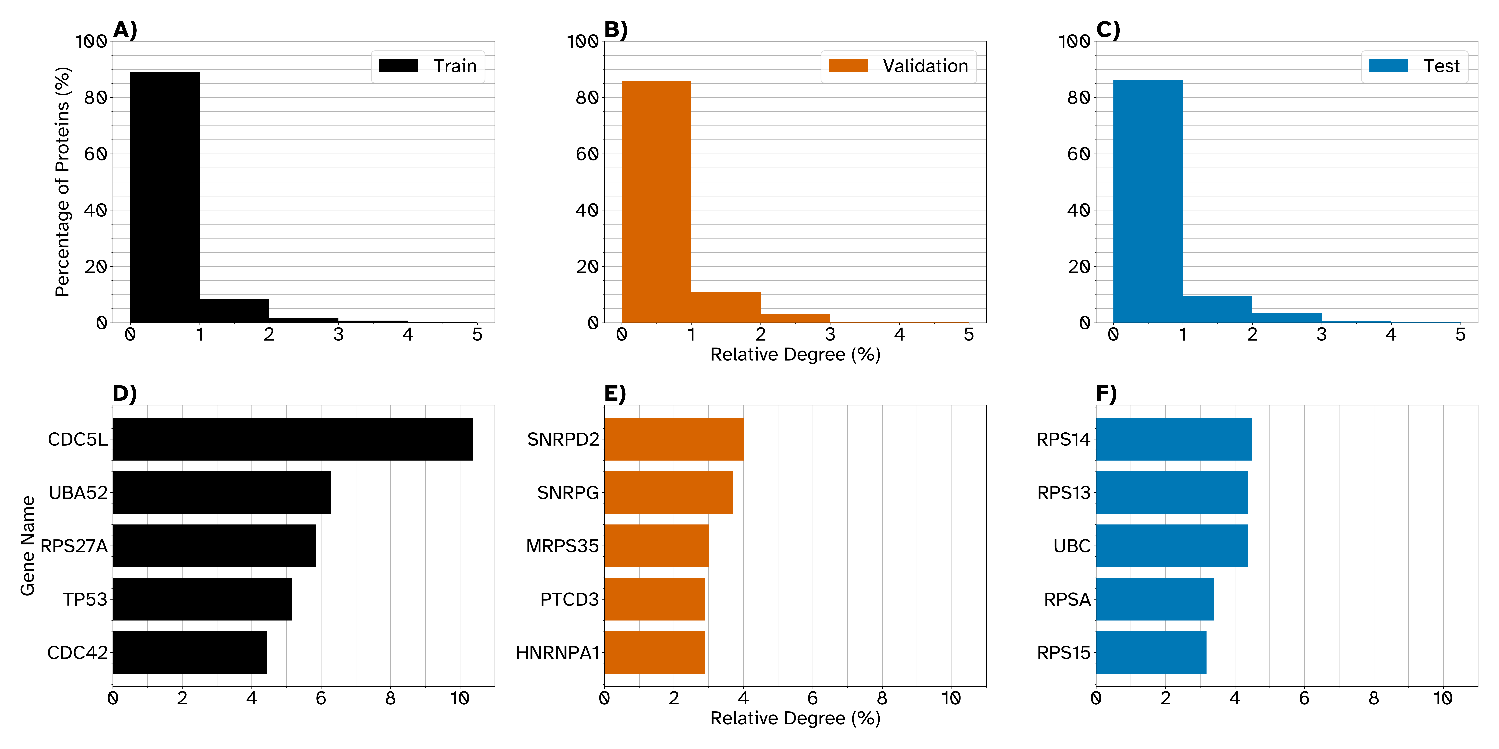
\includegraphics[scale=0.30]{figures/rapppid/rapppid_supp1.png}}
	\caption[Relative Degree of Proteins in the \textit{H. sapiens} \textsc{string} \textsc{c3} dataset.]{\textsf{\textbf{Relative Degree of Proteins in the \textit{H. sapiens} STRING C3 dataset.}} The
distribution of the relative degree of proteins between the three splits of the \textit{H. sapiens} \textsc{string} \textsc{c3} datasets reveal that the vast majority of proteins have a relative degree of less than 1\% \textbf{(A-C)}. The top five proteins with the highest relative degrees are plotted in bar graphs D through F. \textit{CDC5L} has a relative degree of 10.37\%, the highest of the entire dataset. Many of the proteins of high relative degree belong to the families of ribosomal or ribonucleoproteins.}\label{fig:rapppid:degree}
\end{figure}

\begin{figure}[h]
	\centerline{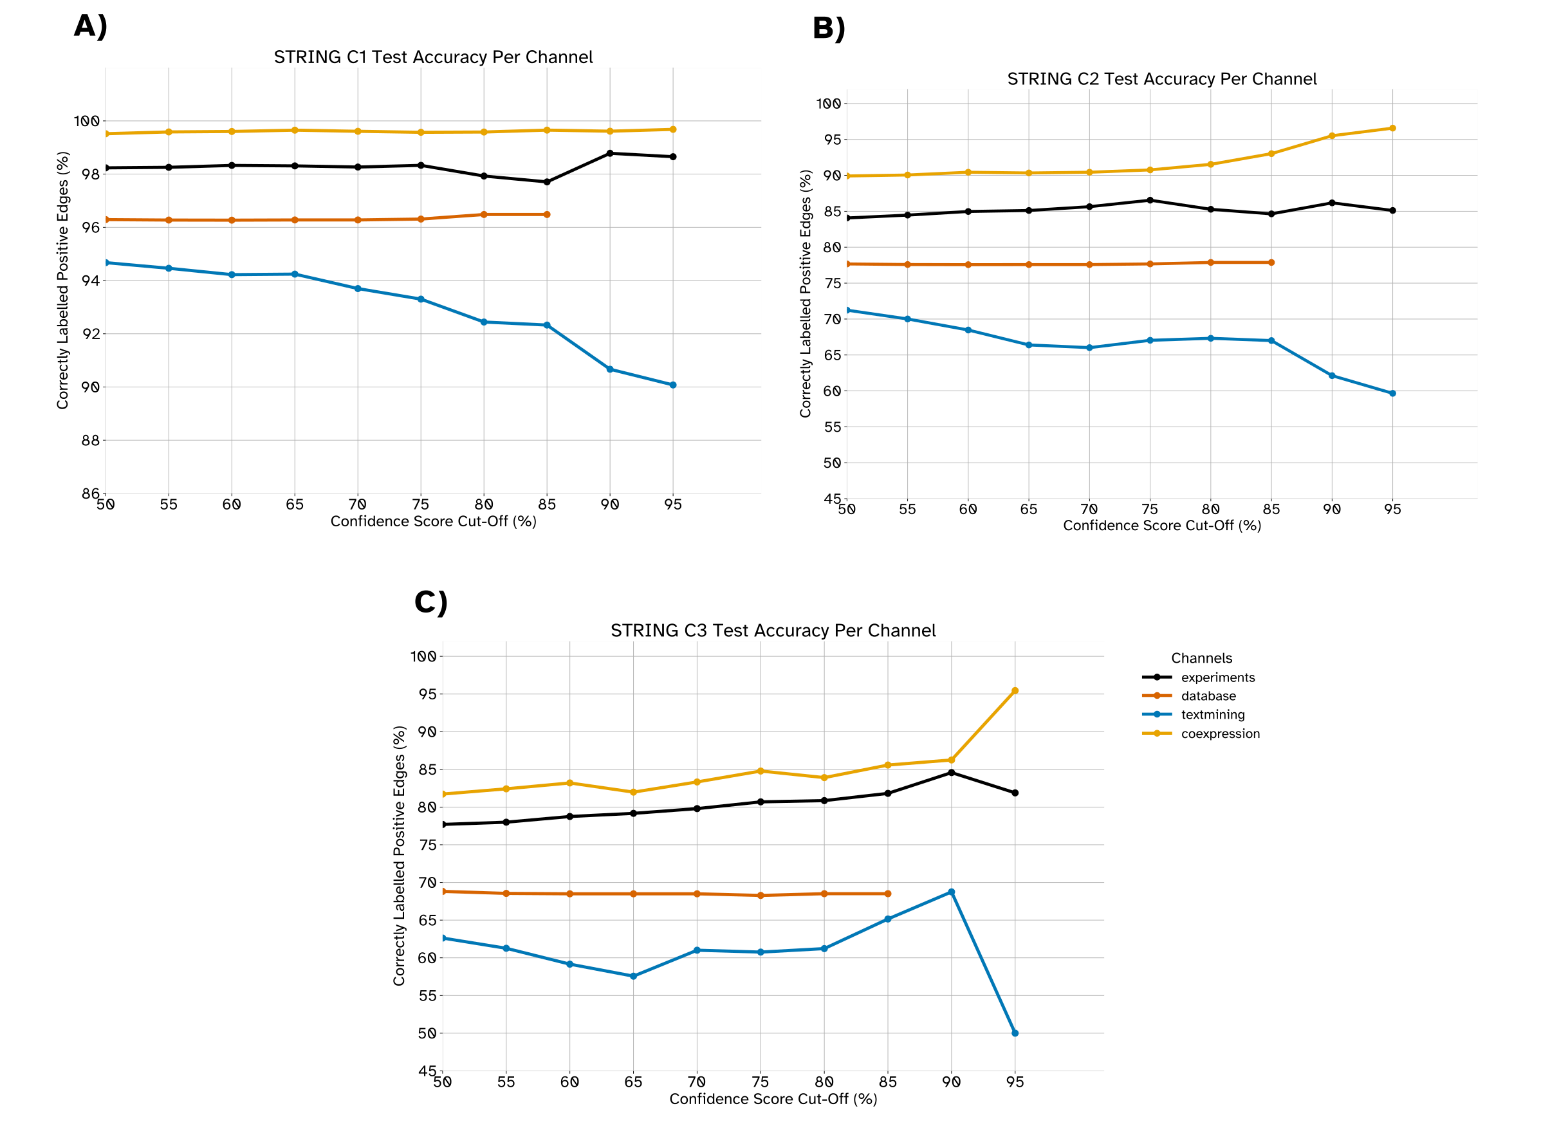
\includegraphics[scale=0.30]{figures/rapppid/rapppid_supp2.png}}
	\caption[Accuracy of positive edges across edge confidence stratified by \textsc{string} channels.]{\textsf{\textbf{Accuracy of positive edges across edge confidence stratified by STRING channels.}} The percentage of correctly labelled positive edges are plotted for each major \textsc{string} channel in the \textsc{c1} \textbf{(A)}, \textsc{c2} \textbf{(B)}, and \textsc{c3} \textbf{(C)} datasets. The x-axis denotes the channel edge confidence cut-off score for each curve’s respective channel.}\label{fig:rapppid:channels_supp}
\end{figure}

\begin{figure}[h]
	\centerline{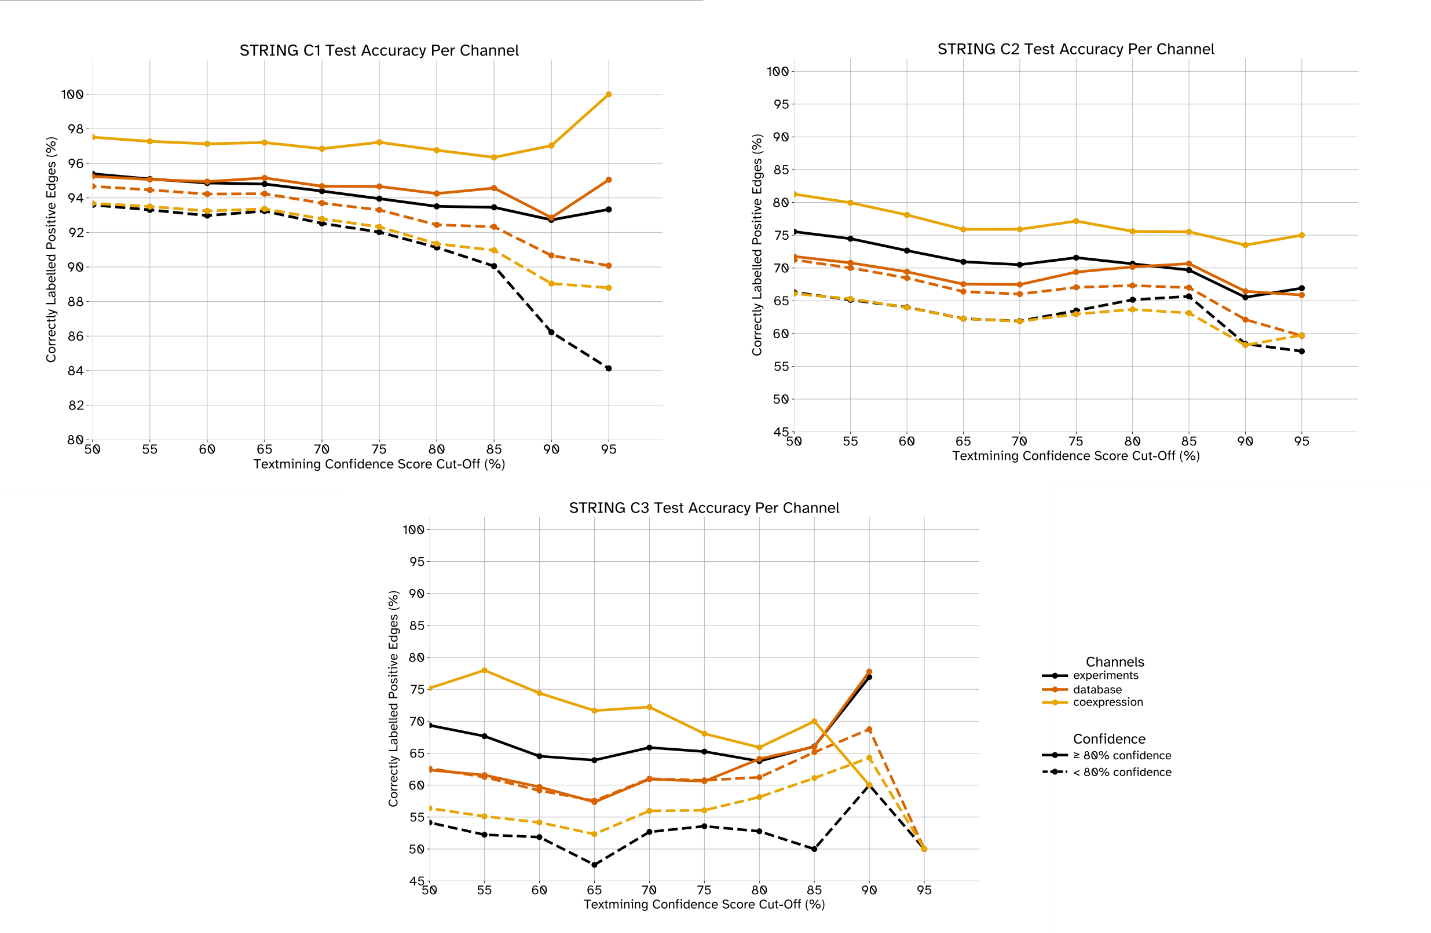
\includegraphics[scale=0.30]{figures/rapppid/rapppid_supp3.png}}
	\caption[Accuracy of positive edges across edge confidence stratified by \textsc{string}
channels.]{\textsf{\textbf{Accuracy of positive edges across edge confidence stratified by STRING channels.}} The percentage of correctly labelled positive edges are plotted for each major \textsc{string} channel, excluding text-mining. Edges are excluded according to the text-mining confidence threshold (x-axis). The solid curves include edges which have a channel confidence $\leq 80\%$ for the channel indicated by the curve’s colour. Dashed curves conversely include edges whose channel confidence is 80\% for the channel indicated by the curve’s colour. Data shown reflects the \textsc{c1} model/dataset in panel \textbf{(A)}, the \textsc{c2} model/dataset in panel \textbf{(B)}, and the \textsc{c3} model/dataset in panel \textbf{(C)}.}\label{fig:rapppid:channels_supp2}
\end{figure}

\begin{figure}[h]
	\centerline{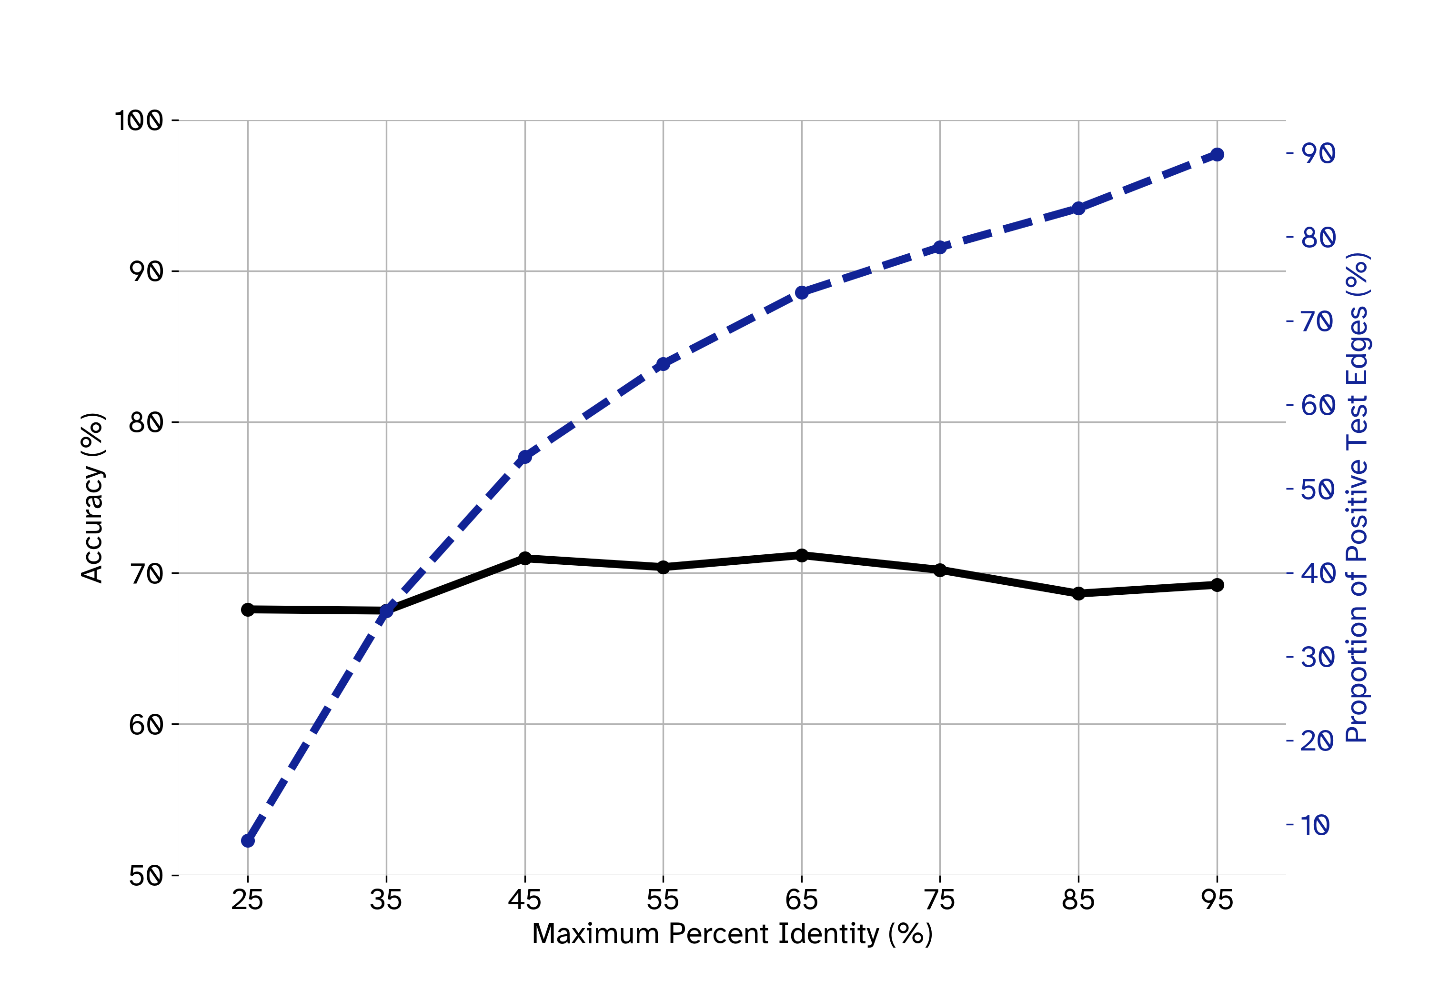
\includegraphics[scale=0.30]{figures/rapppid/rapppid_supp4.png}}
	\caption[Accuracy of positive edges as a function of similarity between testing and
training proteins in \textsc{c3}.]{\textsf{\textbf{Accuracy of positive edges as a function of similarity between testing and training proteins in C3.}} The similarity between testing and training proteins was measured using their percent identity as computed by \textsc{ncbi}'s \textsc{psi-blast} software. The highest percent identity between any training protein and a testing protein in a testing edge was considered to be that testing edge's ``maximum percent identity''. The percentage of accurately labelled positive edges (black curve, left y-axis) is reported for edges with maximum percent identities lower than the threshold reported on the x-axis. The proportion of testing edges for each threshold values is reported by the dashed blue curve and the right y-axis.}\label{fig:rapppid:similarity_supp}
\end{figure}

\begin{figure}[h]
	\centerline{\includegraphics[scale=0.05]{figures/rapppid/rapppid_supp5.png}}
	\caption[Distribution of Interaction Probabilities of Trastuzumab and Pertuzumab with
all Proteins of the Human Proteome as Predicted by \textsc{rapppid}.]{\textsf{\textbf{Distribution of Interaction Probabilities of Trastuzumab and Pertuzumab with all Proteins of the Human Proteome as Predicted by \textsc{rapppid}.}} The probability of interaction between the antibodies (Trastuzumab and Pertuzumab) and each protein in the human proteome (according to \textsc{string}) were individually predicted using \textsc{rapppid}. The distribution of these probabilities is here shown for interactions between Trastuzumab (top) and Pertuzumab (bottom). The quartiles are marked by blue dashed lines, and illustrate that the majority of proteins have a probability of interacting less than 35.9\% and 28.8\% for Trastuzumab and Pertuzumab, respectively. The dotted orange line demarks where \textsc{her2} is positioned in the distribution, holding a probability of interaction of 98.8\% and 95.1\% with Trastuzumab and Pertuzumab, respectively.}\label{fig:rapppid:trastuzumab}
\end{figure}

  %\begin{singlespace}
\chapter[Supplementary Material for ``Causal single-cell RNA-seq simulation, in silico perturbation, and GRN inference benchmarking using GRouNdGAN-Toolkit'']{Supplementary Material for ``Causal single-cell RNA-seq simulation, in silico perturbation, and GRN inference benchmarking using GRouNdGAN-Toolkit''}
\markboth{Appendix B. Supplementary Material for GRouNdGAN-Toolkit}{Appendix B. Supplementary Material for GRouNdGAN-Toolkit}%
\end{singlespace}

\setcounter{table}{0}
\renewcommand{\thetable}{S\arabic{table}}
\renewcommand{\thefigure}{S\arabic{figure}}
\figuresection{Supplementary Material for ``Causal single-cell RNA-seq simulation, in silico perturbation, and GRN inference benchmarking using GRouNdGAN-Toolkit''}

\section*{Supplementary Methods}\label{sec:intrepppid_supp_methods}
\subsection*{Preparing strict PPI datasets}
A \textsc{ppi} dataset $\mathcal{D}$ is a set of interacting protein-pairs reflecting binary interactions $D_i \in \mathcal{D}$. $\mathcal{D}$ is partitioned into three mutually disjoint subsets: a training subset ($\mathcal{D}_\textrm{Tr}$), a testing subset ($\mathcal{D}_\textrm{Te}$), and a validation subset ($\mathcal{D}_\textrm{V}$). Let $P_\textrm{Tr}$, $P_\textrm{Te}$, and $P_\textrm{V}$ be the set of proteins present in $\mathcal{D}_\textrm{Tr}$, $\mathcal{D}_\textrm{Te}$, and
$\mathcal{D}_\textrm{V}$, respectively, and let $\mathcal{P}$ be the collection of protein sets ${P_\textrm{Tr}, P_\textrm{Te},  P_\textrm{V}}$.

We define a strict \textsc{ppi} dataset as a dataset $\mathcal{D}$ (with its collection of protein sets $\mathcal{P}$) that fulfills the following two criteria.

\textit{Criterion 1 --- Distinct Protein Identity}\\
The resulting protein sets $P_\textrm{Tr}, P_\textrm{Te},  P_\textrm{V}$ of the dataset must be mutually disjoint:

$$
\forall Q, R \in \mathcal{P} \; Q \cap R = \emptyset \; \textrm{if} \; Q \neq R.
$$

\textit{Criterion 2 --- Distinct Sequence Identity}\\
The amino acid sequence of any pair of proteins belonging to different protein subsets must have a sequence identity no greater than 90\%:

$$
\forall Q, R \in \mathcal{P}, \; \forall q \in Q \; \forall r \in R \; f(q,r) \leq 90\% \; \textrm{if} \; Q \neq R
$$

where $f(\cdot,\cdot)$ is some protein sequence identity function.

For the datasets used in the experiments carried out herein, the UniRef90 identifiers provided by UniProt were used to determine sequence identity, and as such we adopt the same definition of sequence identity [1,2].

\textit{High-confidence examples of \textsc{ppi}s}\\
To minimize our exposure to falsely labelled \textsc{ppi}s, we required a database that provided information regarding the confidence of the interactions. We selected the \textsc{string} database as the source of \textsc{ppi}s for our datasets as it is large, contains information for many species, and integrates confidence scores from a number of modalities [3]. We exclude all \textsc{ppi}s which do not have a combined confidence score greater or equal to 90\%, and only include \textsc{ppi}s which are
classified as ``physical interactions''. \textsc{ppi} information for seven species were included in our analyses.

\begin{table}[h]
	 {\begin{tabular}{@{}llll@{}}\toprule 
			Scientific Name & Common Name & \textsc{ncbi} Taxon \textsc{id} & Patristic Distance\\
                            &                &                     & from \textit{H.~sapiens}\\\midrule
			\textit{Homo sapiens} & Human & 9606 & 0.000 \\
            \textit{Mus musculus} & House mouse & 10090 & 0.0455 \\
            \textit{Danio rerio} & Zebrafish & 7955 & 0.156 \\
            \textit{Drosophila melanogaster} & Fruit fly & 7227 & 0.358 \\
            \textit{Caenorhabditis elegans} & Nematode & 6239 & 0.455 \\
            \textit{Arabidopsis thaliana} & Thale cress & 3702 & 0.693 \\
            \textit{Saccharomyces cerevisiae} & Baker's yeast & 4932 & 0.734 \\
			\midrule
	\end{tabular}}{}
\end{table}

Patristic distance is a measure of the divergence of two lineages. Patristic distances were computed using DendroPy and data from i\textsc{tol} [4,5].

\textit{Negative examples of \textsc{ppi}s}\\
As \textsc{intrepppid} is a supervised method, it requires examples of pairs of proteins which do not interact (negative examples), in addition to pairs which do (positive examples). Obtaining negative examples of \textsc{ppi}s is a fraught process as there exists no one agreed upon ``gold standard'' of proteins which do not interact with one another. While many approaches for obtaining negative \textsc{ppi} examples have been devised over the years, evidence has shown that many of these methods introduce a great amount of bias [6]. For this reason, we opted to sample pairs of proteins in a uniformly random manner to represent our negative examples. For the training set, negatives were randomly drawn without replacement from the set $N_\textrm{Tr}$, defined as:

$$
N_\textrm{Tr} = \left\{\{p,q\} | p \in P_\textrm{Tr}, q \in P_\textrm{Tr}, \{p,q\} \notin \mathcal{D} \right\}
$$

Negative examples for the testing and validation sets were drawn from $N_\textrm{Te}$ and $N_\textrm{V}$, which were similarly defined as the set of protein-pairs of $P_\textrm{Te}$ and $P_\textrm{V}$, respectively, which were not in $\mathcal{D}$ (\textit{i.e.}, were not considered interacting in the dataset).

Random sampling of protein-pairs requires the fewest assumptions about the distribution of negative pairs, thereby reducing bias, albeit at the risk of false-negatives. Through the exclusion of known interactions from $N_\textrm{Tr}$, however, we’ve reduced the likelihood of drawing false-negatives.

\textit{Considerations for cross-species datasets}\\
For experiments herein, it was necessary to prepare datasets suitable for testing the cross-species task. Namely, we needed to construct training sets whose \textit{ppi}s were composed of proteins of one species, and many corresponding testing sets each belonging to a different species. All combinations of the training set and the many testing sets must satisfy both Criteria 1 and 2. The first criterion is typically met \textit{de facto}, as protein identifiers between species normally do not overlap. In order for the second criterion to be met, positive and negative interactions of proteins that do not satisfy Criterion 2 were excluded from the datasets.
\newpage
\section*{Supplementary Tables and Figures}
\subsection*{Tables}

\subsubsection*{Table S1}
\label{sec:intrepppid_supp_s1}

Table S1 is provided as a separate .xlsx spreadsheet file.
\addtocounter{table}{1}

Its caption is as follows:

\begin{displayquote}
\begin{singlespace}
Statistics of each dataset used in this study. Datasets are listed by source organism and random seed used to generate the random splits.
\end{singlespace}
\end{displayquote}

\begin{tcolorbox}
    This file is available for download from \textsc{oup} Briefings in Bioinformatics:\\ \href{https://doi.org/10.1093/bib/bbae405}{https://doi.org/10.1093/bib/bbae405}.
\end{tcolorbox}

\newpage

\begin{table}[!h]
\centering
	\caption[Hyperparameters used to train \textsc{intrepppid} in all experiments.]{\textsf{\textbf{Hyperparameters used to train INTREPPPID in all experiments.}}} \label{tab:intrepppid_supp_hyperparameters} {\begin{tabular}{@{}ll@{}}\toprule 
			Hyperparameter & Value  \\\midrule
			Batch Size & 80 \\
            Embedding Size & 64 \\
            Number of \textsc{rnn} Layers & 2 \\
            \textsc{rnn} Drop-connect Rate & 0.3 \\
            Embedding Drop-out Rate & 0.3\\
			\midrule
	\end{tabular}}{}

\end{table}

\newpage

\subsubsection*{Table S3}
\label{sec:intrepppid_supp_s3}

Table S3 is provided as a separate .xlsx spreadsheet file.
\addtocounter{table}{1}

Its caption is as follows:

\begin{displayquote}
\begin{singlespace}
Confusion matrix statistics of various methods trained and tested on \textit{H.~sapiens} data.
\end{singlespace}
\end{displayquote}

\begin{tcolorbox}
    This file is available for download from \textsc{oup} Briefings in Bioinformatics:\\ \href{https://doi.org/10.1093/bib/bbae405}{https://doi.org/10.1093/bib/bbae405}.
\end{tcolorbox}

\newpage
\begin{table}[!h]
\centering
	\caption[Performance of \textsc{intrepppid} tested on increasing negative-to-positive ratios.]{\textsf{\textbf{Performance of INTREPPPID trained on \textit{H.~sapiens} datasets with a 1:1 negative-to-positive interaction ratios, and tested on increasing negative-to-positive ratios.}}} \label{tab:intrepppid_supp_neg_ratio} {\begin{tabular}{@{}llllll@{}}\toprule 
			Negative:Positive & 1:1 & 2:1 & 10:1 & 50:1 & 100:1  \\\midrule
			\textsc{auroc} Mean & 0.752 & 0.723 & 0.733 & 0.728 & 0. 733 \\
            \textsc{auroc} Std & 0.017 & 0.004 & 0.006 & 0.011 & 0.004\\
			\midrule
	\end{tabular}}{}

\end{table}

\newpage

\subsubsection*{Table S5}
\label{sec:intrepppid_supp_s5}

Table S5 is provided as a separate .xlsx spreadsheet file.
\addtocounter{table}{1}

Its caption is as follows:

\begin{displayquote}
\begin{singlespace}
Metrics of various \textsc{ppi} inference methods trained on \textit{H.~sapiens} data, and tested on various species. Each model was tested on a total of twenty-four dataset: four different random testing splits for each six different organism. The metrics reported here are averaged over all four datasets, with the standard deviation between the four datasets also reported. The first worksheet (\textsc{auroc}) reports the area-under-the-receiver-operator-curve (\textsc{auroc}). The second worksheet (\textsc{ap}) reports the average-precision. The third worksheet (F150) reports the $F_1$ measure with a 50\% threshold.
The fourth worksheet (MCC50) reports the Matthew's correlation coefficient (\textsc{MCC}) with a 50\% threshold. The fifth and final worksheet (Brier) reports the Brier score. Higher values indicate better performance for all metrics but the Brier score, where the inverse is true.
\end{singlespace}
\end{displayquote}

\begin{tcolorbox}
    This file is available for download from \textsc{oup} Briefings in Bioinformatics:\\ \href{https://doi.org/10.1093/bib/bbae405}{https://doi.org/10.1093/bib/bbae405}.
\end{tcolorbox}

\newpage

\begin{table}[!h]
\centering
	\caption[Performance of \textsc{intrepppid} with scrambled and not scrambled orthologue information.]{\textsf{\textbf{Performance of INTREPPPID trained on \textit{H.~sapiens} datasets with scrambled and not
scrambled orthologue information.}} Bold-face indicates the best value for each metric.} \label{tab:intrepppid_supp_scramble} {\begin{tabular}{@{}lllll@{}}\toprule 
			Scramble Status & Test \textsc{auroc} & Test \textsc{ap} & Test \textsc{mcc}@50\% & Test Brier Score  \\\midrule
			Not Scrambled & \textbf{0.761} & \textbf{0.737} & \textbf{0.378} & \textbf{0.198} \\
            Scrambled & 0.524 & 0.527 & 0.017 & 0.314 \\
			\midrule
	\end{tabular}}{}

\end{table}

\newpage

\begin{table}[!h]
\centering
	\caption[Change in \textsc{intrepppid} performance when omitting orthology data.]{\textsf{\textbf{Performance of INTREPPPID when trained on \textit{H.~sapiens} dataset which omits orthology data for the seven species tested below, relative to the performance of INTREPPPIED trained on dataset which includes all orthology data available.}}} \label{tab:intrepppid_supp_no_ortho} {\begin{tabular}{@{}lllll@{}}\toprule 
			Testing Dataset & Test \textsc{auroc} & Test \textsc{ap} & Test \textsc{mcc}@50\% & Test Brier Score  \\\midrule
			\textit{H.~sapiens} & -0.49\% & -1.36\% & -9.00\% & 2.00\% \\
            \textit{M. musculus} & -13.21\% & -14.79\% & 34.39\%  & 21.06\% \\
            \textit{D. rerio} & -13.69\% & -16.16\% & -38.85\%  & 8.66\% \\
            \textit{D. melanogaster} & -11.29\% & -11.67\% & -26.48\%  & 5.81\% \\
            \textit{C. elegans} & -12.51\% & -17.58\% & -13.45\%  & -0.73\% \\
            \textit{S. cerevisiae} & -9.21\% & -15.12\% & -13.31\%  & -3.17\% \\
            \textit{A. thaliana} & -9.29\% & -11.55\% & -30.75\%  & 5.39\% \\
			\midrule
	\end{tabular}}{}
\end{table}

\newpage

\subsubsection*{Table S8}
\label{sec:intrepppid_supp_s8}

Table S8 is provided as a separate .xlsx spreadsheet file.
\addtocounter{table}{1}

Its caption is as follows:

\begin{displayquote}
\begin{singlespace}
Results of the statistical over-expression analysis conducted on top \textsc{intrepppid}-unique positive hits for seven species. The statistical over-expression of \textsc{go} Molecular Function annotations among proteins that make up the top \textsc{intrepppid}-unique positive hits was measured relative to the proteins which make up the testing dataset for the specific species tested. A Fisher's Exact test was performed by the online \textsc{panther} Classification System. The fold enrichment, raw $p$ values, and corrected $p$ values using Benjamini-Hochberg false-discover rate (\textsc{fdr}) correction are reported for \textsc{go} Molecular Function annotations found to be over-expressed. Only results with a corrected $p$ value of less than 0.05 are included in this table. Each worksheet in the spreadsheet is labelled with a species name, and reports the over-expression analysis for the testing dataset that belongs to that species.
\end{singlespace}
\end{displayquote}

\begin{tcolorbox}
    This file is available for download from \textsc{oup} Briefings in Bioinformatics:\\ \href{https://doi.org/10.1093/bib/bbae405}{https://doi.org/10.1093/bib/bbae405}.
\end{tcolorbox}

\newpage

\begin{table}[!h]
\centering
	\caption[Analysis of online availability of \textsc{ppi}-related tools.]{\textsf{\textbf{Analysis of 22 randomly sampled articles advertising online PPI-related tools and the online availability of said tools as of January 2024.}} Articles were found using the SemanticScholar.org academic search engine with the search terms ``protein-protein interaction website''.} \label{tab:intrepppid_supp_links} {\begin{tabular}{@{}lllll@{}}\toprule 
			\textsc{doi} & Corpus\textsc{id} & Year Published & \textsc{uri} & Status  \\\midrule
			\texttt{10.1093/nar/gks434} & 9914396 & 2012 & \href{http://dropnet.isima.fr/}{Link} & \textcolor{red}{Dead} \\
            \texttt{10.1007/978-1-0716-0892-0\_12} & 226218388 & 2020 & \href{http://wodaklab.org/iRefWeb}{Link} & \textcolor{ForestGreen}{Alive} \\
            \texttt{10.1007/978-1-4939-9873-9\_12} & 203659921 & 2020 & \href{https://oncoppi.emory.edu/}{Link} & \textcolor{ForestGreen}{Alive} \\
            \texttt{10.1515/jib-2006-27} & 16195629 & 2006 & \href{http://biomis.fh-hagenberg.at/isp/primos}{Link} & \textcolor{red}{Dead} \\
            \texttt{10.1089/adt.2013.506} & 12969509 & 2013 & \href{http://primos.fh-hagenberg.at/}{Link} & \textcolor{red}{Dead} \\
            \texttt{10.1093/nar/gkx333} & 31083221 & 2017 & \href{https://proteins.plus/}{Link} & \textcolor{ForestGreen}{Alive} \\
            \texttt{10.1371/journal.pone.0056228} & 2014834 & 2013 & \href{http://www.canevolve.org/}{Link} & \textcolor{red}{Inaccessible\textsuperscript{1}} \\
            \texttt{10.1093/nar/gkp335} & 3041302 & 2009 & \href{https://meme.nbcr.net/}{Link} & \textcolor{red}{Inaccessible\textsuperscript{2}} \\
            \texttt{10.1093/NAR/GKG056} & 15003973 & 2003 & \href{http://www.bind.ca/}{Link} & \textcolor{red}{Dead} \\
            \texttt{10.1109/CBMS.2008.113} & 19040991 & 2009 & \href{http://212.189.149.159:8080/mcl_service}{Link} & \textcolor{red}{Dead} \\
            \texttt{10.1093/nar/gkx385} & 3268569 & 2017 & \href{http://dynomics.pitt.edu/}{Link} & \textcolor{ForestGreen}{Alive} \\
            \texttt{10.1093/nar/gkac1000} & 253479599 & 2022 & \href{https://string-db.org/}{Link} & \textcolor{ForestGreen}{Alive} \\
            \texttt{10.7726/AJBCB.2014.1003} & 12004796 & 2014 & \href{http://bicompute.appspot.com/}{Link} & \textcolor{ForestGreen}{Alive} \\
            \texttt{10.1093/bioinformatics/btn584} & 206340817 & 2009 & \href{http://www.bioinformatics.sussex.ac.uk/protorp}{Link} & \textcolor{red}{Dead} \\
            \texttt{10.1186/1471-2105-11-S10-P1} & 40906621 & 2010 & \href{http://www.compbio.dundee.ac.uk/pips}{Link} & \textcolor{ForestGreen}{Alive} \\
            \texttt{10.1093/bioinformatics/btx312} & 4420839 & 2017 & \href{https://www.iitm.ac.in/bioinfo/PROXiMATE/}{Link} & \textcolor{ForestGreen}{Alive} \\
            \texttt{10.1155/2013/737591} & 5548876 & 2013 & \href{http://nrf2.elte.hu/}{Link} & \textcolor{red}{Dead} \\
            \texttt{10.1038/nmeth.1931} & 52853893 & 2012 & \href{http://www.imexconsortium.org/}{Link} & \textcolor{ForestGreen}{Alive} \\
            \texttt{10.3389/fgene.2021.722198} & 229549097 & 2020 & \href{https://rbc-dsai-iitm.github.io/NetGenes/}{Link} & \textcolor{ForestGreen}{Alive} \\
            \texttt{10.1093/nar/gkv1072} & 8843610 & 2015 & \href{https://www.bindingdb.org/rwd/bind/index.jsp}{Link} & \textcolor{ForestGreen}{Alive} \\
            \texttt{10.1093/nar/gkt1210} & 560515 & 2013 & \href{https://ipfam.org/}{Link} & \textcolor{red}{Dead} \\
			\midrule
	\end{tabular}}{}
\end{table}

\textsuperscript{1}Presents a login page with no context or registration option.\\
\textsuperscript{2}URI resolves but the described online web server is not present.

\newpage
\subsection*{Figures}

\begin{figure}[h]
	\centerline{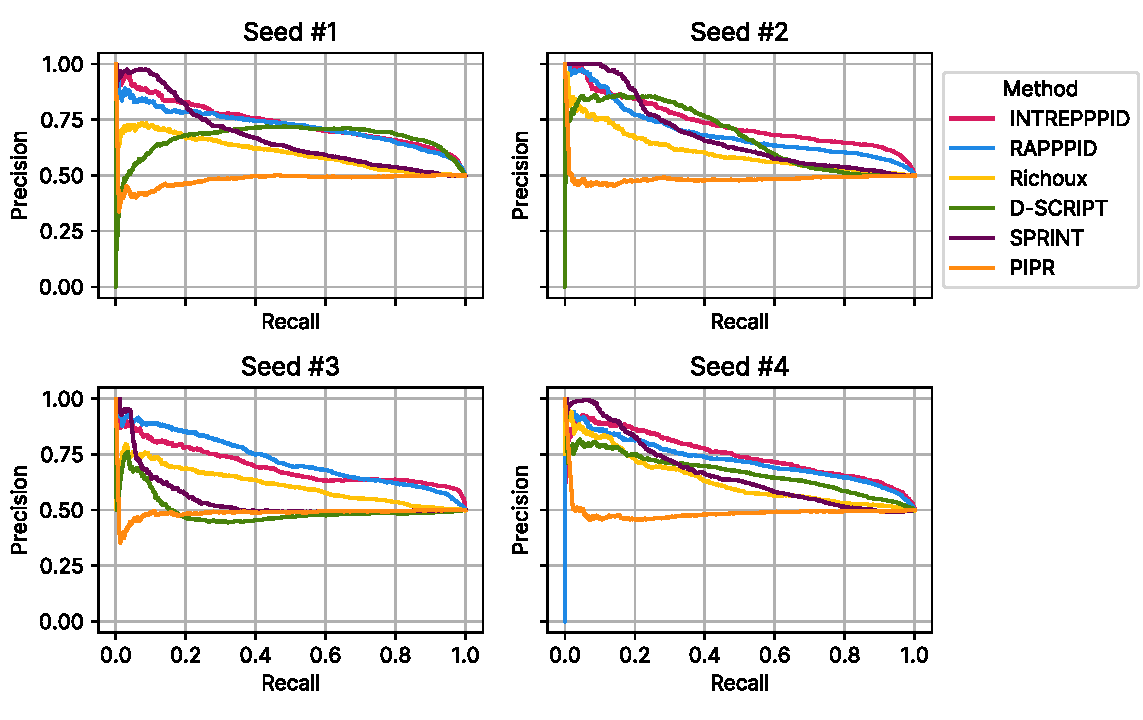
\includegraphics[scale=0.8]{figures/intrepppid/pr_curve3.pdf}}
	\caption[Precision-Recall curves of various \textsc{ppi} inference methods]{\textsf{\textbf{Precision-Recall curves of various PPI inference methods tested and trained on \textit{H.~sapiens} data.}} Each panel reports the Precision-Recall curve for one of four different datasets.}\label{fig:intreppid_supp_pr}
\end{figure}

\begin{figure}[h]
	\centerline{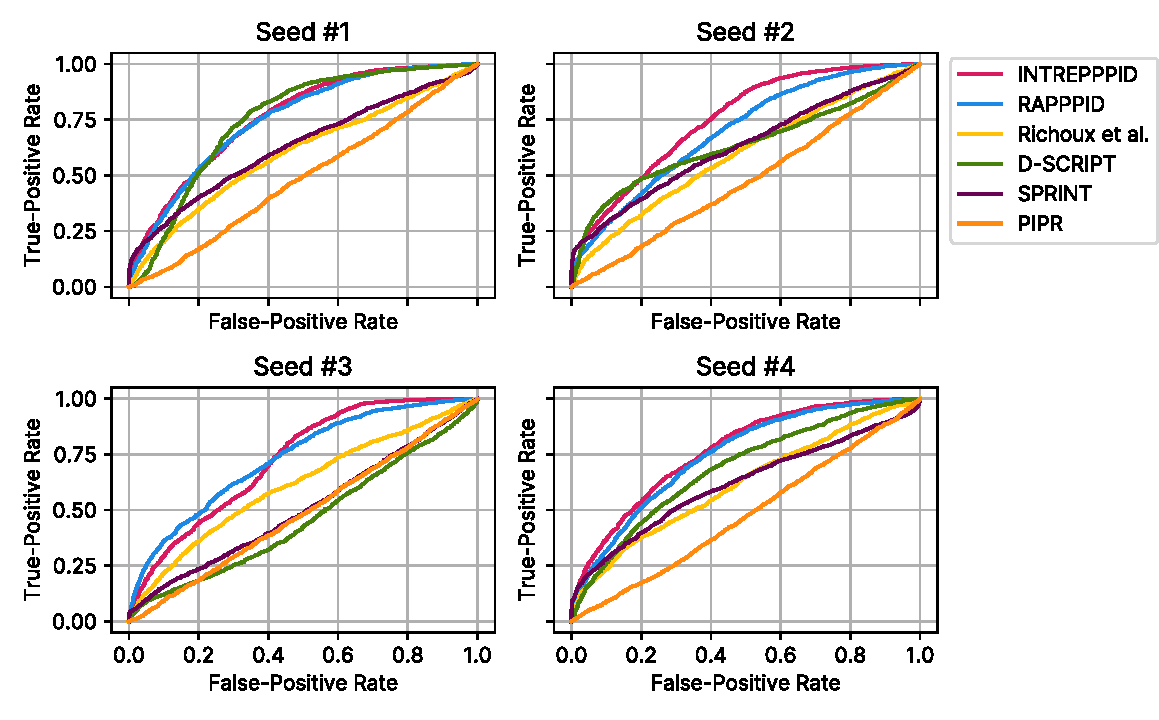
\includegraphics[scale=0.8]{figures/intrepppid/roc3.pdf}}
	\caption[Receiver-Operator curves of various \textsc{ppi} inference methods]{\textsf{\textbf{Receiver-Operator curves of various PPI inference methods tested and trained on \textit{H.~sapiens} data.}} Each panel reports the Receiver-Operator curve for one of four different datasets.}\label{fig:intreppid_supp_roc}
\end{figure}

\begin{figure}[h]
	\centerline{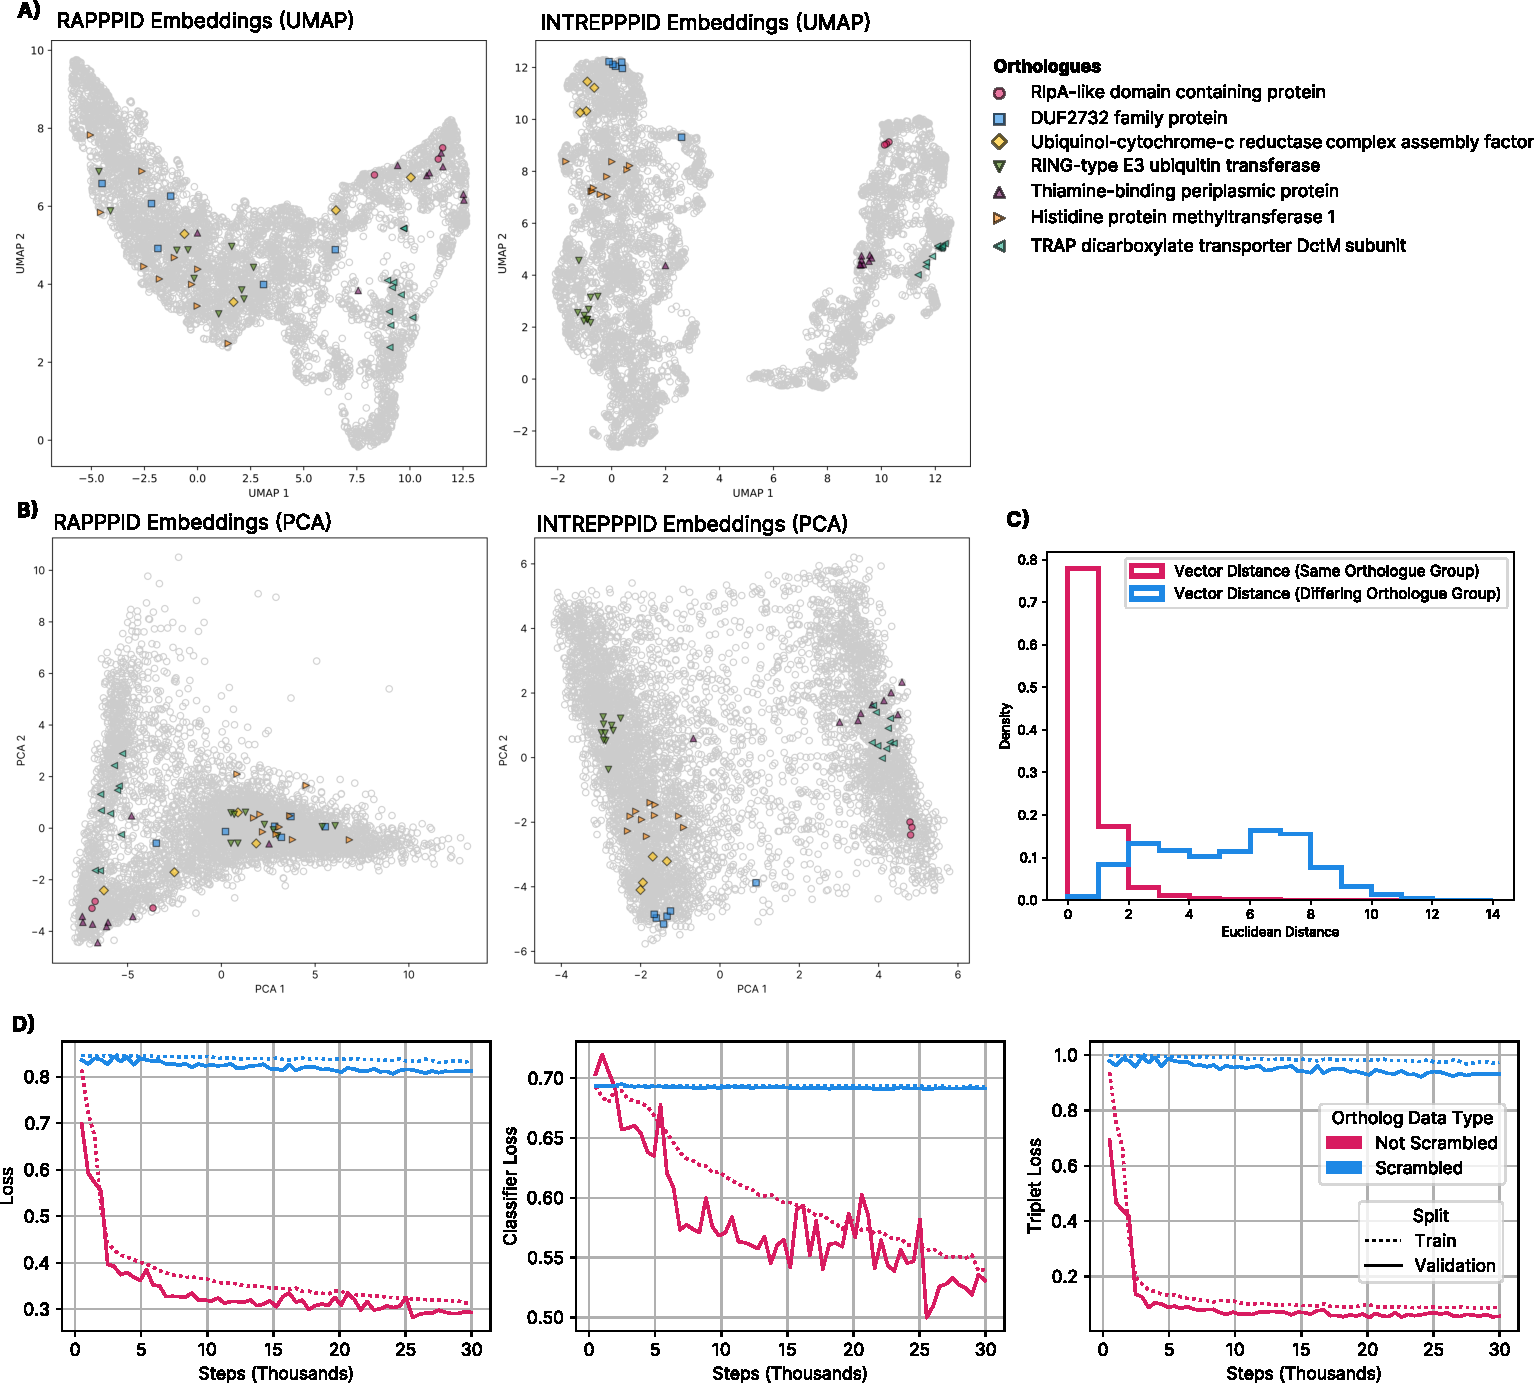
\includegraphics[scale=0.6]{figures/intrepppid/scramble_oma4.pdf}}
	\caption[The effect of orthologous locality task.]{\textsf{\textbf{The effect of orthologous locality task.}} \textbf{(A-B)} A random sample of protein sequences
from various species were embedded using \textsc{rapppid} (left) and \textsc{intrepppid} (right) and projected onto a 2D space using the \textbf{(A)} \textsc{umap} and \textbf{(B)} \textsc{pca} algorithm. Distinct markers indicate proteins which belong to the same orthologous group according to the \textsc{oma} database. The orthologous groups shown were chosen at random. \textbf{(C)} Histogram of the Euclidean distance between \textsc{intrepppid} latent vector representations of protein sequences of the same orthologous group (magenta) and of differing orthologous groups (blue). \textbf{(D)} Training (dotted line) and validation loss (solid line) of \textsc{intrepppid} trained on \textit{H.~sapiens} datasets whose orthologue data is ``scrambled'' (blue) and ``not scrambled'' (magenta). The overall loss (left), the loss of the classification network (middle), and the loss of the triplet network (right) are plotted above, demonstrating that the ``scrambled'' dataset fails to optimize any aspect of the loss in any appreciable way.}\label{fig:intreppid_supp_scramble} \end{figure}
\clearpage
\section*{References}
\begin{enumerate}
    \item  Suzek BE, Wang Y, Huang H, \textit{et al.} UniRef clusters: a comprehensive and scalable alternative for improving sequence similarity searches. \textit{Bioinformatics} 2015; 31:926–932
    
    \item The UniProt Consortium, Bateman A, Martin M-J, \textit{et al.} UniProt: the Universal Protein Knowledgebase in 2023. \textit{Nucleic Acids Research} 2023; 51:D523–D531

    \item Szklarczyk D, Kirsch R, Koutrouli M, \textit{et al.} The \textit{string} database in 2023: protein–protein association networks and functional enrichment analyses for any sequenced genome of interest. \textit{Nucleic Acids Research} 2023; 51:D638–D646

    \item Sukumaran J, Holder MT. DendroPy: a Python library for phylogenetic computing. \textit{Bioinformatics} 2010; 26:1569–1571

    \item Letunic I, Bork P. Interactive Tree Of Life (i\textsc{tol}) v5: an online tool for phylogenetic tree display and annotation. \textit{Nucleic Acids Research} 2021; 49:W293–W296

    \item Ben-Hur A, Noble WS. Choosing negative examples for the prediction of protein-protein interactions. \textit{BMC Bioinformatics} 2006; 7:S2–S2
\end{enumerate}

  %--------------------------------------------%
  %% Bibliography %%
  %--------------------------------------------%
  \bibliographystyle{unsrt}         % bib style
  \bibliography{bibliography/refs}  % load bib file



\end{document}